%--------------------------------------------------------------------------
%
%  M.Sc. Thesis
%  Satellite using ARL
%  By: Ali Baniasad
%
%--------------------------------------------------------------------------



\documentclass[oneside,a4paper,12pt]{book}
\usepackage{array,booktabs,makecell,graphicx} % rotatebox in graphicx
\newcolumntype{R}[1]{>{\raggedleft\arraybackslash}p{#1}}   % right-aligned, fixed width
\newcolumntype{C}[1]{>{\centering\arraybackslash}p{#1}}    % centered, fixed width
\usepackage{booktabs,tabularx,siunitx,threeparttable}

\sisetup{
	reset-text-series = false,
	text-series-to-math = true,
	reset-text-family = false,
	text-family-to-math = true,
	table-number-alignment = center,
	round-mode = places,
	round-precision = 2
}
\setlength{\tabcolsep}{3.5pt}
\renewcommand{\arraystretch}{1.15}
\newcolumntype{L}{>{\raggedleft\arraybackslash}X} % right-align Persian scenario names

% -------------------------------------------------------
%  Common Styles and Formattings
% -------------------------------------------------------


\usepackage{amssymb,amsmath}
\usepackage[colorlinks,linkcolor=blue,citecolor=blue]{hyperref}
\usepackage[usenames,dvipsnames]{pstricks}
\usepackage{graphicx,subfigure,wrapfig}
\usepackage{geometry}
\usepackage[mathscr]{euscript}
\usepackage{graphicx,subfigure,wrapfig}
\usepackage{multicol}
\usepackage{multirow}
\usepackage{tikz}
\tikzset{
	frame/.style={
		rectangle, draw,
		text width=6em, text centered,
		minimum height=4em,drop shadow,fill=white,
		rounded corners,
	},
	line/.style={
		draw, -{Latex},rounded corners=3mm,
	}
}
\usetikzlibrary{arrows.meta,shadows,positioning}
\usepackage[figureposition=bottom,tableposition=top,font={small,bf},labelfont=bf]{caption}

\usepackage{algorithmicx,algorithm}

\usepackage[localise=on,extrafootnotefeatures]{xepersian}
\usepackage[noend]{algpseudocode}


%------------------------ Algorithm ------------------------------------

\newenvironment{الگوریتم}[1]
	{\bigskip\bigskip\begin{algorithm}\caption{#1} \label{الگوریتم: #1}\vspace{0.5em}\begin{algorithmic}[1]}
	{\end{algorithmic}\vspace{0.5em}\end{algorithm}\bigskip}
	

\renewcommand{\algorithmicfor}{{به ازای}}
\renewcommand{\algorithmicwhile}{{تا وقتی}}
\renewcommand{\algorithmicdo}{\hspace{-.2em}:}
\renewcommand{\algorithmicif}{{اگر}}
\renewcommand{\algorithmicthen}{\hspace{-.2em}:}
\renewcommand{\algorithmicelse}{{در غیر این صورت:}}
%\renewcommand{\algorithmicelsif}{{در غیر این صورت اگر: }}
\renewcommand{\algorithmicreturn}{{برگردان}}
\renewcommand{\algorithmiccomment}[1]{$\triangleleft$ \emph{#1}}
\renewcommand{\algorithmicrequire}{\textbf{ورودی:}}
\renewcommand{\algorithmicensure}{\textbf{خروجی:}}

\newcommand{\اگر}{\If}
\newcommand{\وگرنه}{\Else}
\newcommand{\وگر}{\ElsIf}
\newcommand{\پایان‌اگر}{\EndIf}
\newcommand{\به‌ازای}{\For}
\newcommand{\پایان‌به‌ازای}{\EndFor}
\newcommand{\تاوقتی}{\While}
\newcommand{\پایان‌تاوقتی}{\EndWhile}
\newcommand{\دستور}{\State}
\newcommand{\دستورک}{\Statex}
\newcommand{\توضیحات}{\Comment}
\newcommand{\برگردان}{\Return}
\renewcommand{\ورودی}{\Require}
\newcommand{\خروجی}{\Ensure}



% -------------------- Page Layout --------------------


%\newgeometry{top=3cm,right=3cm,left=2.5cm,bottom=3cm,footskip=1.25cm}
\newgeometry{margin=1in,bottom=1.1in,footskip=.4in}

\renewcommand{\baselinestretch}{1.4}
\linespread{1.6}
\setlength{\parskip}{0.45em}

%\fancyhf{}
%\rhead{\leftmark}
%\lhead{\thepage}


% -------------------- Fonts --------------------

\settextfont[
Scale=1.09,
Extension=.ttf, 
Path=styles/fonts/,
BoldFont=XB NiloofarBd,
ItalicFont=XB NiloofarIt,
BoldItalicFont=XB NiloofarBdIt
]{XB Niloofar}

\setdigitfont[
Scale=1.09,
Extension=.ttf, 
Path=styles/fonts/,
BoldFont=XB NiloofarBd,
ItalicFont=XB NiloofarIt,
BoldItalicFont=XB NiloofarBdIt
]{XB Niloofar}

\defpersianfont\sayeh[
Scale=1,
Path=styles/fonts/
]{XB Kayhan Pook}


% -------------------- Styles --------------------


\SepMark{-}
\renewcommand{\labelitemi}{$\small\bullet$}



% -------------------- Environments --------------------


\newtheorem{قضیه}{قضیه‌ی}[chapter]
\newtheorem{لم}[قضیه]{لم}
\newtheorem{ادعا}[قضیه]{ادعای}
\newtheorem{مشاهده}[قضیه]{مشاهده‌ی}
\newtheorem{نتیجه}[قضیه]{نتیجه‌ی}
\newtheorem{مسئله}{مسئله‌ی}[chapter]
\newtheorem{تعریف}{تعریف}[chapter]
\newtheorem{مثال}{مثال}[chapter]


\newenvironment{اثبات}
	{\begin{trivlist}\item[\hskip\labelsep{\em اثبات.}]}
	{\leavevmode\unskip\nobreak\quad\hspace*{\fill}{\ensuremath{{\square}}}\end{trivlist}}

\newenvironment{alg}[2]
	{\begin{latin}\settextfont[Scale=1.0]{Times New Roman}
	\begin{algorithm}[t]\caption{#1}\label{algo:#2}\vspace{0.2em}\begin{algorithmic}[1]}
	{\end{algorithmic}\vspace{0.2em}\end{algorithm}\end{latin}}


% -------------------- Titles --------------------


\renewcommand{\listfigurename}{فهرست شکل‌ها}
\renewcommand{\listtablename}{فهرست جدول‌ها}
\renewcommand{\bibname}{\rl{{مراجع}\hfill}} 


% -------------------- Commands --------------------


\newcommand{\IN}{\ensuremath{\mathbb{N}}} 
\newcommand{\IZ}{\ensuremath{\mathbb{Z}}} 
\newcommand{\IQ}{\ensuremath{\mathbb{Q}}} 
\newcommand{\IR}{\ensuremath{\mathbb{R}}} 
\newcommand{\IC}{\ensuremath{\mathbb{C}}} 

\newcommand{\set}[1]{\left\{ #1 \right\}}
\newcommand{\seq}[1]{\left< #1 \right>}
\newcommand{\ceil}[1]{\left\lceil{#1}\right\rceil}
\newcommand{\floor}[1]{\left\lfloor{#1}\right\rfloor}
\newcommand{\card}[1]{\left|{#1}\right|}
\newcommand{\setcomp}[1]{\overline{#1}}
\newcommand{\provided}{\,:\,}
\newcommand{\divs}{\mid}
\newcommand{\ndivs}{\nmid}
\newcommand{\iequiv}[1]{\,\overset{#1}{\equiv}\,}
\newcommand{\imod}[1]{\allowbreak\mkern5mu(#1\,\,\text{پیمانه‌ی})}

\newcommand{\poly}{\mathop{\mathrm{poly}}}
\newcommand{\polylog}{\mathop{\mathrm{polylog}}}
\newcommand{\eps}{\varepsilon}

\newcommand{\lee}{\leqslant}
\newcommand{\gee}{\geqslant}
\renewcommand{\leq}{\lee}
\renewcommand{\le}{\lee}
\renewcommand{\geq}{\gee}
\renewcommand{\ge}{\gee}

\newcommand{\مهم}[1]{\textbf{#1}}
\renewcommand{\برچسب}{\label}

\newcommand{\REM}[1]{}
\renewcommand{\حذف}{\REM}
\newcommand{\لر}{\lr}
\newcommand{\کد}[1]{\lr{\tt #1}}
\newcommand{\پاورقی}[1]{\footnote{\lr{#1}}}



% -------------------- Dictionary --------------------


\newcommand{\dicalphabet}[1]{
\begin{minipage}{\columnwidth}
	\centerline{\noindent\textbf{\large #1 }}
	\vspace{.5em}
\end{minipage}
\nopagebreak[4]
}

\newcommand{\dic}[2]{\noindent  #2 \dotfill  \lr{#1} \\ }


% ------------------------------ Images and Figures --------------------------

\graphicspath{{figs/}}
\setlength{\intextsep}{0pt}  % for float boxes
\renewcommand{\psscalebox}[1]{}  % for LaTeX Draw

\newcommand{\floatbox}[2]
	{\begin{wrapfigure}{l}{#1}
	\centering #2 \end{wrapfigure}}

\newcommand{\centerfig}[2]
	{\centering\scalebox{#2}{\input{figs/#1}}}

\newcommand{\fig}[3]
	{\floatbox{#3}{\centerfig{#1}{#2}}}

\newcommand{\centerimg}[2]
	{\vspace{1em}\begin{center}\includegraphics[width=#2]{figs/#1}\end{center}\vspace{-1.5em}}

\NewDocumentCommand{\img}{m m o}
	{\begin{wrapfigure}{l}{\IfValueTF{#3}{#3}{#2}}
	\centering\includegraphics[width=#2]{figs/#1}\end{wrapfigure}}




% -------------------------------------------------------
%  Custom Definitions
% -------------------------------------------------------


\newcommand{\OPT}{\ensuremath{\mathop{\mathrm{OPT}}}}
\newcommand{\APX}{\ensuremath{\mathop{\mathrm{APX}}}}
\newcommand{\ALG}{\ensuremath{\mathop{\mathrm{ALG}}}}



\begin{document}


% -------------------- Front Pages --------------------


% -------------------------------------------------------
%  Thesis Information
% -------------------------------------------------------

\newcommand{\ThesisType}
{پروژه کارشناسی}
\newcommand{\ThesisTitle}
{هدایت  یادگیری تقویتی مقاوم مبتنی بر بازی دیفرانسیلی در محیط‌های پویای چندجسمی با پیشران کم}
\newcommand{\ThesisAuthor}
{علی بنی اسد}
\newcommand{\ThesisSupervisor}
{دکتر هادی نوبهاری}
\newcommand{\ThesisAdvisor}
{استاد مشاور}
\newcommand{\ThesisExaminer}
{استاد ممتحن}
\newcommand{\ThesisDate}
{تیر 1401}
\newcommand{\ThesisDepartment}
{دانشکده‌ی مهندسی هوافضا}
\newcommand{\ThesisMajor}
{مهندسی کنترل}
\newcommand{\ThesisUniversity}
{دانشگاه صنعتی شریف}


% -------------------------------------------------------
%  English Information
% -------------------------------------------------------

\newcommand{\EnglishThesisType}{Bachelor Thesis}

\newcommand{\EnglishThesisTitle}{Robust Reinforcement Learning Differential Game Guidance in Low-Thrust, Multi-Body Dynamical Environments}

\newcommand{\EnglishThesisAuthor}{Ali BaniAsad}

\newcommand{\EnglishThesisSupervisor}{Dr.Hadi Nobahari}

\newcommand{\EnglishThesisDate}{July 2022}

\newcommand{\EnglishThesisDepartment}{Department of Aerospace Engineering}

\newcommand{\EnglishThesisUniversity}{Sharif University of Technology}

%\pagestyle{empty}


\pagestyle{empty}

\begin{center}


\includegraphics[scale=0.25]{front/template/images/logo}

\begin{large}

\vspace{-0.2cm}
\ThesisUniversity \\[-0.3em]
\ThesisDepartment

\vspace{0.5cm}

\ThesisType \\[-0.3em]
\ThesisMajor

\end{large}

\vspace{1cm}

{عنوان:}\\[1.2em]
{\LARGE\textbf{\ThesisTitle}}

\vspace{1cm}

{نگارش:}\\[.5em]
{\large\textbf{\ThesisAuthor}}

\vspace{0.7cm}

{استاد راهنما:}\\[.5em]
{\large\textbf{\ThesisSupervisor}}

\vspace{1.3cm}

\ThesisDate

\end{center}

\newpage


\pagestyle{empty}

\begin{center}


\includegraphics[scale=0.75]{front/template/images/besmellah.jpg}

\end{center}

%\newpage
‌  % بسم‌الله

\pagestyle{empty}

\begin{large}
\setlength{\parindent}{0pt}
\begin{center}

{\large\bf به نام خدا}

\ThesisUniversity

\vspace{-0.1cm}
\ThesisDepartment

\vspace{2.5em}
\textbf{\large\ThesisType}

\end{center}

\vspace{1em}

\begin{center}
	{\large عنوان: \\ \ThesisTitle}
\end{center}

\vspace{.3em}

{\large نگارش: \ThesisAuthor}

\vspace{1.5cm}

\textbf{کمیته‌ی ممتحنین}

\vspace{1em}
\begin{tabular}{p{8.5cm}r}
استاد راهنما: \ThesisSupervisor & امضاء: \\[1.8em]
استاد ممتحن: \ThesisAdvisor & امضاء: \\[1.8em]
استاد ممتحن: \ThesisExaminer & امضاء: \\[2em]
& تاریخ:
\end{tabular}

\end{large}

\newpage
  % تصویب‌نامه
%\include{front/template/declaration}  % اظهارنامه

\pagestyle{plain}
\pagenumbering{tartibi}
%‎\DefaultMathsDigits


% -------------------------------------------------------
%  Acknowledgments
% -------------------------------------------------------


\begin{center}
\مهم{سپاس}
\end{center}

\بدون‌تورفتگی از استاد بزرگوارم جناب آقای دکتر نوبهاری که با کمک‌ها و راهنمایی‌های بی‌دریغشان، بنده را در انجام این پروژه یاری داده‌اند، تشکر و قدردانی می‌کنم.
%همچنین، از دوست عزیزم جناب آقای مهندس رضا پردال که نظرات ارزشمند او همواره راهگشای مشکلات بنده بود، تشکر می‌کنم.
از پدر دلسوزم ممنونم که در انجام این پروژه مرا یاری نمود. در نهایت در کمال تواضع، با تمام وجود بر دستان مادرم بوسه می‌زنم که اگر حمایت بی‌دریغش، نگاه مهربانش و دستان گرمش نبود برگ برگ این دست نوشته و پروژه وجود نداشت.

\صفحه‌جدید
  % تقدیر و تشکر

% -------------------------------------------------------
%  Abstract
% -------------------------------------------------------


\pagestyle{plain}

\begin{وسط‌چین}
\مهم{چکیده}
\end{وسط‌چین}

\بدون‌تورفتگی در این پژوهش، از یک روش مبتنی بر نظریه بازی\LTRfootnote{Game Theory} به‌منظور کنترل وضعیت استند سه درجه آزادی چهارپره استفاده شده‌است. 
%در این روش سیستم و اغتشاش دو بازیکن اصلی در نظر گرفته شده‌است. هر یک از دو بازیکن سعی می‌کنند امتیاز خود را  با کمترین هزینه افزایش دهند که در اینجا،  وضعیت استند امتیاز بازیکن‌ها در نظر گرفته ‌شده‌است. 
در این روش بازیکن اول سعی در ردگیری ورودی مطلوب می‌کند و بازیکن دوم با ایجاد اغتشاش سعی در ایجاد خطا  در ردگیری بازیکن اول می‌کند.
در این روش انتخاب حرکت با استفاده از تعادل نش\LTRfootnote{Nash Equilibrium} که با فرض بدترین حرکت دیگر بازیکن است،  انجام می‌شود.
این روش نسبت به اغتشاش ورودی و همچنین نسبت به عدم قطعیت مدل‌سازی  می‌تواند مقاوم باشد.
% از روش ارائه‌شده برای کنترل یک استند سه درجه آزادی چهارپره که به نوعی یک آونگ معكوس نیز هست، استفاده شده‌است. 
برای ارزیابی عملکرد این روش ابتدا شبیه‌سازی‌هایی در محیط سیمولینک انجام شده‌است و سپس، با پیاده‌سازی روی استند سه درجه آزادی صحت عملکرد کنترل‌کننده تایید شده‌است. 

\پرش‌بلند
\بدون‌تورفتگی \مهم{کلیدواژه‌ها}: 
چهارپره،  بازی دیفرانسیلی، نظریه بازی، تعادل نش، استند سه درجه آزادی، مدل‌مبنا، تنظیم‌کننده مربعی خطی 
\صفحه‌جدید



% -------------------- Table of Contents --------------------

\tableofcontents \newpage
\listoftables \newpage
\listoffigures \newpage
\listofalgorithms \newpage


% -------------------- Chapters --------------------
\pagestyle{plain}
\pagenumbering{arabic}

% Chapter 1: Introduction
\chapter{مقدمه}

%\section{انگیزه پژوهش}
%\section{انگیزه پژوهش}\label{sec:motivation}
%
%در دههٔ اخیر، گرایش روزافزون مأموریت‌های فضایی به استفاده از سامانه‌های سبک‌وزن و کم‌هزینه—از مدارگردهای زیردولتی گرفته تا صورت‌های متنوع ماهواره‌های مکعبی (CubeSat)—تقاضا برای روش‌های هدایت و کنترل خودکار و تضمین‌کنندهٔ امنیت مأموریت را به شکلی چشمگیر افزایش داده است. در این مأموریت‌ها، منابع پیشرانی محدود و محدودیت‌های توان پردازشی، هر دو، محیط طراحی را به سمت راهکارهایی سوق می‌دهند که ضمن بهینگی مصرف سوخت، نسبت به عدم‌قطعیت‌های «محیط سه‌جسمی محدود»ootnote{Circular Restricted Three‑Body Problem یا CRTBP} و آشفتگی‌های ناشی از خطاهای مدل و اختلالات بیرونی (مانند فشار تابشی خورشید و نامحوری جرم سیاره) مقاوم باشند.  
%
%از سوی دیگر، قرارگیری در نقطه‌های لاگرانژی \lr{\(L_1\)} و \lr{\(L_2\)} سامانهٔ خورشید–زمین، فرصت‌های اکتشافی بی‌سابقه‌ای—از رصد پس‌زمینهٔ کیهانی گرفته تا هواشناسی فضایی—فراهم کرده است، اما پایداری ذاتی پایین این نواحی، نیازمند راهبردهای ایمن نگه‌دارنده (station‑keeping) با دورهٔ کنترل کوتاه و واکنش سریع است. روش‌های کلاسیک همچون \lr{LQR} و هدایت بهینهٔ \lr{(OC)}, اگرچه در بسیاری از کاربردهای زمینی کارآمد بوده‌اند، در حضور سامانه‌های غیرخطی با ابعاد بالا و دینامیک آشوب‌گونهٔ CRTBP مستعد فروپاشی عملکرد (performance degradation) هستند؛ به ویژه زمانی که مدل دقیق جرم‌های آسمانی در دسترس نباشد یا حافظهٔ محاسباتی فضاپیما محدود شود.
%
%پیشرفت‌های اخیر در \lr{Machine Learning} و به طور خاص \lr{Reinforcement Learning (RL)}، چشم‌اندازی نو را پیش روی پژوهشگران سامانه‌های کنترلی قرار داده است؛ چراکه RL با یادگیری گام‌به‌گام از تعامل با محیط می‌تواند سیاست‌هایی را بیابد که نیازی به مدل صریح از دینامیک نداشته باشند. با این حال، اکثر کاربردهای موجود RL در حوزهٔ فضایی به صورت «تک‌عاملی» (Single‑Agent) و عمدتاً در چارچوب مسئله‌های \lr{Markov Decision Process (MDP)} صورت پذیرفته‌اند، حال آنکه تولد سامانه‌های مشارکتی و سناریوهای چندفازی (مانند مانورهای گله‌ای ماهواره‌ها یا مشارکت زمینی–مداری) مستلزم فریم‌ورک‌هایی چندعاملی است که بتواند برهم‌کنش‌های رقابتی–همکاری و همچنین نامعلومی‌های مشترک را مدیریت کند. الگوریتم‌های \lr{Multi‑Agent RL (MARL)}، به ویژه هنگامی که با تئوری بازی‌های دیفرانسیلی ترکیب شوند، قابلیتی فراهم می‌کنند تا عامل‌ها در برابر بدترین حالت اختلالات احتمالی (adversarial disturbances) آموزش ببینند و از آن طریق، ضریب اطمینان مأموریت ارتقا یابد.
%
%با وجود این پتانسیل، خلئی محسوس در ادبیات وجود دارد:  
%\begin{itemize}
%	\item \textbf{عدم تصریح چارچوبی جامع برای RL مقاوم در CRTBP} \cite{Naasz2022,Gabriel2023}؛ اکثر پژوهش‌ها یا به پایداری نقاط تعادل ساده اکتفا کرده یا تقارن کامل سامانه را فرض می‌کنند.
%	\item \textbf{نبود مقایسهٔ منصفانه بین الگوریتم‌های گرادیان‑سیاست (مانند TD3 و SAC) و روش‌های مبتنی بر توابع ارزش توزیعی} در سناریوهای فضایی گسسته–پیوسته.
%	\item \textbf{فقدان گزارش کمی از مزیت سوختی RL نسبت به کنترلرهای بهینهٔ کلاسیک}؛ آماری چون $\Delta m/m <1\%$ غالباً کیفی گزارش می‌شوند.
%\end{itemize}
%
%بر همین اساس، هدف از این پژوهش عبارت است از:  
%\begin{enumerate}
%	\item توسعهٔ یک چارچوب \textit{مقاوم} \lr{MARL}—بر پایهٔ بازی دیفرانسیلی صفرمجموع—برای مسئلهٔ هدایت کم‌پیشران در CRTBP، به نحوی که در برابر خطاهای مدل جرم اولیه و فشار تابشی تا $\pm20\,\%$ پایداری را حفظ کند.
%	\item طراحی یک تابع پاداش ترکیبی \(R=\alpha J_\text{fuel}+\beta J_\text{deviation}+\gamma J_\text{slack}\) که به طور هم‌زمان، مصرف سوخت و انحراف از مدار نامی را کمینه و محدودیت‌های پیشران را رعایت کند.
%	\item ارائهٔ مقایسهٔ جامع بین کنترلر پیشنهادی و رویکرد \lr{LQR/LQG}، از حیث $\Delta v$، تعداد اشتعال و خطای پسا‑ماموریت.
%\end{enumerate}
%
%تحقق این اهداف نه تنها می‌تواند سهم قابل‌توجهی در کاهش هزینه‌های مأموریت و افزایش عمر عملیاتی فضاپیماها داشته باشد، بلکه دانش طراحی کنترلی برای محیط‌های غیرخطی آشوبی را یک گام به افق «استقلال کامل تصمیم‌گیری در فضا» نزدیک‌تر می‌کند. به طور خاص، چارچوب ارائه شده قابلیت آن را دارد که در آینده به سادگی به سامانه‌های سه‌بعدی \lr{CR3BP} یا حتی دینامیک‌های چندجرمی تعمیم یابد، بدون آنکه نیاز به بازنویسی ساختار اصلی شبکهٔ عصبی باشد.
%
\section{انگیزه پژوهش}\label{sec:motivation}


%در دو دههٔ اخیر، چشم‌انداز مأموریت‌های فضایی به‌‌واسطهٔ کوچک‌سازی سامانه‌ها، پیشرفت الکترونیک ارزان‌قیمت و افزایش دسترس‌پذیری پرتابْ‌بارها، تغییر محسوسی را تجربه کرده است. از پروژه‌‌های علمی بین‌سیاره‌ای با محدودیت‌های منابع گرفته تا منظومه‌های پرشمارهٔ ماهواره‌ای در مدار زمین، همگی با چالش مشترکِ «هدایت بهینه در حضور عدم‌قطعیت» روبه‌رو هستند. در مسیرهای ترا-لونا و به‌طور خاص ناحیه‌های ناپایدار لاگرانژی در مدل «مسئلهٔ سه‌جسمی کروی محدود و دایروی» (CRTBP)، سامانهٔ کنترل باید قادر باشد با پیشران کم‌تراست (\emph{low‐thrust}) و underactuated، پایداری ایستا و کارایی مصرف سوخت را توأمان تضمین کند.  
%
%در عین حال، ظهور الگوریتم‌های یادگیری تقویتی عمیق (DRL) دریچهٔ تازه‌ای به‌سوی طراحی کنترلگرهای تطبیقی باز کرده است؛ ولی اغلب رویکردهای متداول بر سناریوهای تک‌عاملی و مدل‌های دقیق تکیه دارند. نبودِ استراتژی مقاوم در برابر اغتشاشات مدل و متغیرهای محیطی—از جمله خطای تراستِ موتورهای یونی و تأخیر حسگر—موجب می‌شود عملکرد در شرایط واقعی فاصلهٔ چشمگیری از نتایج شبیه‌سازی ایده‌آل پیدا کند. این پژوهش می‌کوشد شکاف مذکور را با استناد به چارچوب «یادگیری تقویتی چندعاملی مقاوم» پُر کرده و امکان هدایت کم‌سوخت در CRTBP را با وثوق عملیاتی ارتقا دهد.
%
%
%
%
%
%در دو دهه اخیر، چشم‌انداز مأموریت‌های فضایی به‌واسطهٔ کوچک‌سازی سامانه‌ها، پیشرفت الکترونیک ارزان‌قیمت، و افزایش دسترس‌پذیری پرتاب‌بارها، دگرگونی چشمگیری را تجربه کرده است. از پروژه‌های علمی بین‌سیاره‌ای با محدودیت‌های منابع گرفته تا منظومه‌های پرشمار ماهواره‌ای در مدار زمین، همگی با چالش مشترک «هدایت بهینه در حضور عدم‌قطعیت» روبه‌رو هستند. به‌ویژه در مسیرهای فرا-ماهی (ترا-لونا) و ناحیه‌های ناپایدار لاگرانژی در مدل «مسئلهٔ سه‌جسمی کروی محدود و دایروی» (CRTBP)، سامانه کنترل باید بتواند با پیشران کم‌تراست (low-thrust) و underactuated، پایداری ایستا و کارایی مصرف سوخت را توأمان تضمین کند.
%
%در همین حال، ظهور الگوریتم‌های یادگیری تقویتی عمیق (DRL)، افق‌های جدیدی را در طراحی کنترلگرهای تطبیقی گشوده است. با این وجود، اغلب رویکردهای متداول بر سناریوهای تک‌عاملی و مدل‌های دقیق متکی هستند. نبود یک استراتژی مقاوم در برابر اغتشاشات مدل و متغیرهای محیطی—مانند خطای تراست موتورهای یونی و تأخیر حسگر—باعث می‌شود که عملکرد در شرایط واقعی، فاصله چشمگیری از نتایج شبیه‌سازی ایده‌آل داشته باشد. این پژوهش می‌کوشد شکاف مذکور را با بهره‌گیری از چارچوب «یادگیری تقویتی چندعاملی مقاوم» پُر کرده و امکان هدایت کم‌سوخت در CRTBP را با اطمینان عملیاتی ارتقا دهد.

% "Translunar" refers to anything situated or traveling beyond the Moon or its orbit around Earth. It's commonly used in the context of spacecraft missions, particularly the translunar injection (TLI), which is a maneuver that puts a spacecraft on a trajectory towards the Moon. 
در دو دهه‌ی اخیر، ماموریت های فضایی به دلیل کوچک‌سازی سامانه ها، توسعه‌ی وسایل الکترونیک مقرون به صرفه و افزایش ظرفیت های پرتابی، تحولات بنیادینی را تجربه کرده است. از پروژه های علمی بین سیاره‌ایی گرفته تا منظومه های انبوه ماهواره‌ایی در مدارهای پایین زمین، همگی با چالش فراگیر هدایت بهینه در حضور عدم قطعیت های ذاتی مواجه‌اند. در مسیرهای فرا-قمری\LTRfootnote{Trans-lunar}
 و به طور خاص در ناحیه های ناپایدار نقاط لاگرانژ در چارچوب مسئله‌ی سه جسمی کروی محدود و دایروی\LTRfootnote{Circular Restricted Three-Body Problem (CRTBP)}، طراحی سامانه‌ی کنترل مستلزم توانایی تضمین همزمان پایداری ایستا و بهره‌وری سوخت با نیروی پیشران‌کم\LTRfootnote{Low-thrust}
 است.

هم‌راستا با این تحولات، ظهور و گسترش الگوریتم‌های یادگیری تقویتی عمیق\LTRfootnote{Deep Reinforcement Learning (DRL)}، امکانات نوینی را برای طراحی کنترل‌کننده‌های تطبیقی فراهم آورده است. با این حال، غالب رویکردهای رایج بر سناریوهای تک‌عاملی و اتکا به مدل‌های دینامیکی دقیق استوارند. غیاب یک استراتژی مقاوم در مواجهه با اغتشاشات مدل و تغییرات محیطی از جمله خطای تراست در پیشران‌ و تأخیر در سیگنال‌های حسگر منجر به فاصله‌ی چشمگیر عملکرد واقعی از پیش‌بینی‌های حاصل از شبیه‌سازی‌های ایده‌آل می‌گردد. این پژوهش بر آن است تا گسست اشاره‌شده را با بهره‌گیری از چارچوب یادگیری تقویتی چندعاملی مقاوم مرتفع سازد و بدین وسیله، اطمینان هدایت پیشران‌کم در \lr{CRTBP} را افزایش دهد.
\section{تعریف مسئله}\label{sec:problem_statement}
\noindent  در سال‌های اخیر، پیشرفت‌های فناوری در زمینه‌های مختلف، از جمله کنترل پرواز، پردازش سیگنال و هوش مصنوعی، به افزایش کاربردهای ماهواره با پیشران کم در منظومه زمین‐ماه کمک کرده است. ماهواره با پیشران کم می‌تواند برای تعقیب ماهواره‌ها، انتقال مداری و استقرار ماهواره‌ها استفاده شود.
روش‌های هدایت بهینه قدیمی جهت کنترل ماهواره‌ها اغلب نیازمند فرضیات ساده کننده، منابع محاسباتی فراوان و شرایط اولیه مناسب هستند. الگوریتم‌های مبتنی بر یادگیری تقویتی این توانایی را دارند که بدون مشکلات اشاره‌شده هدایت ماهواره را انجام دهند. به‌دلیل ساختار شبکه‌ای، این الگوریتم‌ها می‌توانند امکان محاسبات درونی\LTRfootnote{On-board Computing}  
را فراهم کنند.



هدف از این پژوهش، طراحی سیاست کنترلی برای یک فضاپیما به جرم~$m$ است که در میدان جاذبه‌ی سیستم زمین–ماه به‌صورت دوبُعدی مدل شده‌است. ویژگی‌های این سامانه در ادامه آورده شده‌است.

\begin{itemize}
	\item \textbf{پویایی‌ها:} معادلات حرکت در چارچوب مرجع چرخان به‌صورت مجموعهٔ غیرخطی {$\dot{\boldsymbol{x}} = f(\boldsymbol{x}) + g(\boldsymbol{x})\,\boldsymbol{u}$} نوشته می‌شود که $\boldsymbol{x}\!=\![x,y,\dot x,\dot y]^\top$ بردار حالت و $\boldsymbol{u}$ بردار تراست با کران $\boldsymbol{u}\le u_{\max}$ است.
	\item \textbf{عدم‌قطعیت‌ها:} 
عوامل عدم قطعیت شامل شرایط اولیه تصادفی، اغتشاش در عملگرها، عدم تطابق مدل، مشاهده ناقص، نویز حسگر و تأخیر زمانی هستند که همگی بر عملکرد و پایداری سیستم تأثیر می‌گذارند.
	
%	\item \textbf{قیود مأموریت:} فضای مجاز حرکت حول نقطهٔ لاگرانژی~$L_1$ شعاعی معادل 500~km دارد و میزان مصرف پیشران {$J = \int_0^{t_f}\|\mathbf{u}(t)\|\,\mathrm dt$} باید حداقل شود.
	\item \textbf{صورت بازی دیفرانسیلی:} فضاپیما و طبیعت (اغتشاشات) به‌ترتیب به‌عنوان عامل کنترلی و حریفِ مزاحم مدل شده‌است. مسئله به‌عنوان یک بازی مجموع‌صفر \LTRfootnote{Zero-Sum} 
	در افق زمان محدود {$t_f$} فرمول‌بندی شده‌اند.
\end{itemize}

صورت کامل مسأله را می‌توان با یافتن سیاست {$\pi^\star : \mathcal{X}\to \mathcal{U}$} تعریف کرد که معیار بهینه‌سازی هزینه‌ی تجمعی است.

%رشدمی‌یافته
%\[ J(\pi,\omega) = \mathbb{E}\_{\pi,\omega}\Big[\,\alpha_1\,J\_{\text{fuel}} + \alpha_2\,J\_{\text{deviation}}\Big] \]
%را در بدترین سناریوی اغتشاش~$\omega$ کمینه سازد. ضرایب $\alpha_{1,2}$ اهمیت نسبی سوخت و انحراف مسیر را نشان می‌دهد.

%\section{اهداف و نوآوری}


\section{اهداف و نوآوری پژوهش}\label{sec:objectives}

برای پاسخ به مسألهٔ فوق، این رساله سه هدف اصلی و چهار نوآوری کلیدی را دنبال می‌کند.

\subsection*{اهداف}
\begin{enumerate}
	\item توسعهٔ چارچوب یادگیری تقویتی چندعاملی که در آن فضاپیما و طبیعت به‌عنوان دو عامل با اهداف متضاد مدل می‌شوند.
	\item طراحی تابع پاداش چندبُعدی به‌منظور موازنهٔ مصرف سوخت، پایداری موقعیت و نرمی فرمان.
	\item ارزیابی تجربی روی سناریوهای {{CRTBP}} و مقایسه با کنترلگرهای کلاسیک (MPC, $H_\infty$) و تک‌عاملی (DDPG, TD3).
\end{enumerate}

\subsection*{نوآوری‌ها}
\begin{itemize}
	\item \textbf{آموزش متمرکز–اجرا توزیع‌شده (CTDE)}: استفاده از تخمین‌گر مشترک ارزش برای تقابل عامل–حریف و اعمال سیاست غیرمتمرکز در زمان اجرا.
	\item \textbf{تقریب سیاست مقاوم با شبکهٔ دوگان Q}: به‌کارگیری TD3 دوبخشی برای کاهش گرادیان بایاس ناشی از تابع ارزش بیش‌براورد.
	\item \textbf{شکل‌دهی پاداش مبتنی بر انرژی مدار}: معرفی مولفهٔ انرژی ژاکوبی در پاداش به‌منظور تضمین نزدیکی به سطح انرژی نامی~$C_{J^\ast}$.
	\item \textbf{سامانهٔ شبیه‌سازی متن‌باز}: پیاده‌سازی محیط CRTBP در قالب افزونهٔ {OpenAI Gym} با امکان تزریق عدم‌قطعیت و انتشار کد در GitHub.
\end{itemize}
\section{ساختار گزارش}\label{sec:chapter_content}
در \textbf{فصل دوم} مروری انتقادی بر کارهای مرتبط در هدایت پیشران‌کم و یادگیری تقویتی (تک‌عاملی و چندعاملی) ارائه می‌شود. \textbf{فصل سوم} به مبانی یادگیری تقویتی اختصاص داده شده و الگوریتم‌های \lr{DDPG}، \lr{TD3}، \lr{SAC} و \lr{PPO} مرور می‌شوند. در \textbf{فصل چهارم} چارچوب یادگیری تقویتی چندعاملی و رویکرد \lr{CTDE} تشریح می‌شود و پیوند آن با بازی‌های جمع‌صفر و تعادل نش بیان می‌گردد. در \textbf{فصل پنجم} مدل‌سازی محیط آزمایش بر پایه‌ی \lr{CRTBP} ارائه می‌شود. در \textbf{فصل ششم} طراحی عامل‌ها، فضای حالت/عمل، تابع پاداش و جزئیات آموزش توضیح داده می‌شود. در \textbf{فصل هفتم} چارچوب «سخت‌افزار در حلقه» و ارزیابی زمان‌واقعی گزارش می‌شود. سرانجام، در \textbf{فصل هشتم} نتایج، مقایسه با معیارهای مرجع و مسیرهای آینده‌ی پژوهش جمع‌بندی می‌شود.


% Chapter 2: Literature Review
\chapter{پیشینه پژوهش}

\section{ماموریت‌های بین مداری}
\section{بازی دیفزانسیلی}
\section{یادگیری تقویتی}


از نخستین صورت‌بندی‌های فرایند تصمیم‌گیری مارکُفی در یادگیری تقویتی، پژوهش بر آن بوده‌است که عامل بتواند با اجرای عمل‌ها و دریافت پاداش، سیاستی برای بیشینه‌سازی برگشت بیاموزد. تبیین جامع این چارچوب و الگوریتم‌های بنیادین در ویرایش دوم کتاب سوتون و بارتو به‌مثابه مرجع کلاسیک این حوزه ارائه شده و همچنان مبنای بسیاری از آثار معاصر است \cite{SuttonBarto2018}. % 


دهه‌‌ی ۱۹۹۰ ملادی شاهد شکل‌گیری روش‌هایی بر پایه‌ی ارزش\LTRfootnote{Value}
 نظیر \lr{Q-learning} و نخستین رویکردهای گرادیانِ سیاست بود؛ با وجود این، محدودیت توان محاسباتی و فقدان داده‌ی فراوان، سرعت رشد را کند می‌کرد. ورود شبکه‌های عصبی عمیق نقطه‌ی عطفی بود: مقاله‌ی معروف دیپ‌مایند\LTRfootnote{DeepMind}
  نشان داد که شبکه‌ی \lr{Q} عمیق (\lr{DQN}) می‌تواند صرفاً از پیکسل‌های بازی آتاری سیاستی نزدیک به انسان بیاموزد \cite{Mnih2015}. % 


موفقیت \lr{DQN} نگاه‌ها را به‌سوی گرادیانِ سیاستِ مقیاس‌پذیر معطوف ساخت. بهینه‌سازی ناحیه‌ی اطمینان\LTRfootnote{Trust Region Policy Optimization (TRPO)}
  تضمین بهبود یکنواخت سیاست را فراهم کرد \cite{Schulman2015TRPO}, و روش \lr{A3C} با موازی‌سازی بازیگران، سرعت یادگیری را چند برابر افزایش داد \cite{Mnih2016A3C}. % :contentReference[oaicite:2]{index=2}
کمی بعد، \lr{DDPG} اولین بار گرادیان سیاست قطعی را به فضاهای عمل پیوسته وارد کرد \cite{lillicrap2019continuouscontroldeepreinforcement}. % 
سپس \lr{PPO} با ساده‌سازی قیود \lr{TRPO} و کاهش پارامترهای حساس، به انتخاب پیش‌فرض بسیاری از کاربردهای مهندسی بدل شد \cite{Schulman2017PPO}. % 


با گسترش دامنه‌ی مسائل، پایداری و کاراییِ داده به چالش اصلی بدل گشت. \lr{TD3} نشان داد که کمینه‌کردن میان دو منتقد می‌تواند برآورد بیش‌از‌حد \lr{Q} را مهار کند \cite{Fujimoto2018TD3}, و \lr{SAC} با افزودن بند آنتروپی، هم‌زمان اکتشاف و بازده را بهبود داد \cite{Haarnoja2018SAC}. % :contentReference[oaicite:5]{index=5}


%برای کاهش هزینه‌ی تعامل، موج نوینی از یادگیری تقویتی مدل‌مبنا شکل گرفت. منابع نظام‌مند از این خط پژوهش را بررسی جامع مورلاند و همکاران عرضه می‌کند \cite{Moerland2020MBRLsurvey}، درحالی‌که عامل Dreamer نشان داد می‌توان سیاست را تنها با «تخیل نهفته» در مدل آموخته‌شده به‌روزرسانی کرد \cite{Hafner2019Dreamer}. % :contentReference[oaicite:6]{index=6}


در محیط‌های پرخطر یا گران، جمع‌آوری داده‌ی برخط ناممکن است؛ ازاین‌رو \lr{RL} آفلاین مطرح شد. روش \lr{CQL} با برقراری کران محافظه‌کارانه بر \lr{Q-value} از گرایشِ خارج از توزیع جلوگیری می‌کند \cite{Kumar2020CQL}، و مرور اخیر پراودِنسیو و همکاران طبقه‌بندی جامعی از چالش‌های باز این حوزه ارائه داده است \cite{Prudencio2022OfflineSurvey}. % 


هم‌زمان، دغدغه‌ی ایمنی و تبیین در سامانه‌های واقعی پررنگ شد. مرور سال ۲۰۲۲ نشان می‌دهد که ترکیب قیدهای سخت، توابع جریمه‌ی ریسک و شبیه‌سازی محیط‌های بدبینانه سه خط اصلی ایمنی در \lr{RL} هستند \cite{JMLR:v16:garcia15a}. سلسله‌مراتب نیز با هدف انتقال دانش و تسریع یادگیری مورد توجه قرار گرفت و یک مطالعه‌ی جامع در 
\lr{ACM Computing Surveys}
 چهار چالش کشف زیرکار، یادگیری اشتراک‌پذیر، انتقال و مقیاس‌پذیری را برجسته می‌کند \cite{Ghazalpour2021HRLsurvey}. % 


وقتی چند عامل به‌طور هم‌زمان یاد می‌گیرند، پویایی محیط از دید هر عامل غیرایستا می‌شود. مرور جامع ۲۰۲۴ نشان می‌دهد که چارچوب ناظر متمرکز ـ بازیگر توزیع‌شده\LTRfootnote{Centralized Training with Decentralized Execution (CTDE)}
 راهکاری موثر برای این چالش است و مباحثی چون تخصیص اعتبار جمعی و کشف تعادل را معرفی می‌کند \cite{Song2024MARLsurvey}. % 


پیشرفت‌های یادشده در نهایت به دستاوردهای نمادینی چون \lr{AlphaGo} \cite{Silver2016AlphaGo} و \lr{AlphaStar} \cite{Vinyals2019AlphaStar} انجامیدند که در بازی‌های \lr{Go} و \lr{StarCraft II} از انسان پیشی گرفتند، و معماری توزیع‌شده‌ی \lr{IMPALA} نشان داد که چگونه می‌توان هزاران شبیه‌ساز را با به‌روزرسانی وزن‌های مهم ادغام کرد \cite{Espeholt2018IMPALA}. % 


به‌رغم این جهش‌ها، سه شکاف اساسی پابرجا مانده است: ۱) تضمین ایمنی سخت‌گیرانه در سناریوهای نزدیک‌برخورد، ۲) کاهش وابستگی به داده‌ی پرهزینه یا نایاب از طریق روش‌های مدل‌مبنا و آفلاین، و ۳) مقیاس‌پذیری یادگیری چندعاملی برای سامانه‌های رباتیکی یا فضاپیمای چندگانه. 
%پژوهش حاضر در پی آن است که با تلفیق یادگیری تقویتی مقاوم و چندعاملی در چارچوب سه‌جسمی مداری، به این خلأ پاسخ دهد.

%\section{یادگیری تقویتی چندعاملی}
\section{پیشینهٔ پژوهش یادگیری تقویتی چندعاملی}\label{sec:marl_lit}

امروز یادگیری تقویتی چندعاملی (MARL) به‌عنوان ستون فقرات سامانه‌های هوشمند مشارکتی شناخته می‌شود؛ مسیری که از آزمون‌های سادهٔ دو‌عاملی در دههٔ ۱۹۹۰ آغاز شد و اکنون به معماری‌های توزیع‌شده‌ی در مقیاس هزاران بازیگر رسیده است. این بخش، بدون ورود به زیرشاخه‌های ریز، روایت تاریخیِ پیوسته‌ای ارائه می‌کند که نشان می‌دهد چگونه ایدهٔ \emph{آموزش متمرکز ـ اجرای توزیع‌شده} (CTDE) به پاسخ غالب برای چالش‌های غیرایستایی و انفجار بُعدی بدل شد و چه گام‌هایی هنوز برای ایمنی، ناهمگونی و مقیاس‌پذیری باقی مانده است.

دههٔ ۱۹۹۰ با مقالهٔ \cite{Tan1993} آغاز شد؛ جایی که برای نخستین‌بار مقایسهٔ «عامل‌های مستقل» با «عامل‌های همکار» انجام شد و سود ارتباط و اشتراک تجربه به‌صورت تجربی نشان داده شد. در میانهٔ دههٔ بعد، مرور جامع پانایت و لوک \cite{Panait2005} چشم‌اندازی از مسائل تخصیص اعتبار و غیرایستایی ترسیم کرد و دو مکتب «یادگیری تیمی» و «یادگیری هم‌زمان» را صورت‌بندی نمود.  هم‌زمان، بوشونیـو و همکاران \cite{Busoniu2008} ادبیات متکثر MARL را در قالب اهداف «پایداری دینامیک یادگیری» و «انطباق با رفتار سایر عامل‌ها» جمع‌بندی کردند و راه را برای تحلیل‌های بازی‌محور هموار ساختند. 

ورود شبکه‌های عمیق در سال‌های ۲۰۱۶ـ۲۰۱۷ نقطهٔ عطف بعدی بود؛ «منتقد متمرکز ـ بازیگر توزیع‌شده» در \emph{MADDPG} \cite{Lowe2017} نشان داد که می‌توان از حالت سراسری در فاز آموزش بهره برد، اما سیاست نهایی را صرفاً بر اساس مشاهدات محلی اجرا کرد.  در همان سال، \emph{Value‐Decomposition Networks} یا VDN \cite{Sunehag2017} ایدهٔ تجزیهٔ خطی پاداش را برای تیم‌های کاملاً تعاونی مطرح کرد و راه را برای فاکتوربندی‌های پیش‌رفته گشود. 

۲۰۱۸ شاهد جهش مهمی با \emph{QMIX} بود؛ این روش با اعمال قید تک‌نوا بر ترکیب مقادیر منفرد، هم امکان بهینه‌سازی آف‌پالیسی را فراهم کرد و هم تضمین سازگاری سیاست‌های محلی با ارزش مشترک را برقرار ساخت \cite{Rashid2018}. 

سال ۲۰۱۹ به گسترش بسترهای آزمایش اختصاص یافت. چالش استاندارد \emph{SMAC} بر مبنای StarCraft II معرفی شد و معیار مشترکی برای مقایسهٔ الگوریتم‌ها مهیا کرد \cite{Samvelyan2019SMAC}.هم‌زمان، \emph{QTRAN} \cite{Son2019QTRAN} نشان داد که می‌توان بدون قید خطی یا تک‌نوا، تابع ارزش مشترک را به فضای قابل تجزیه تبدیل کرد. از سوی دیگر، \emph{MAVEN} با افزودن متغیر نهفتهٔ مشترک، کاوش هماهنگ و سلسله‌مراتبی را امکان‌پذیر ساخت \cite{Mahajan2019MAVEN}.  نقطهٔ اوج همان سال، سامانهٔ \emph{AlphaStar} بود که نشان داد ترکیب خودبازی و معماری توزیع‌شده می‌تواند به رتبهٔ گرندمسترِ انسان برساند \cite{Vinyals2019AlphaStar}. 

در ۲۰۲۰ مفهوم «نقش‌های در حال ظهور» با \emph{ROMA} \cite{Wang2020ROMA} معرفی شد تا عامل‌ها بر اساس شباهت رفتاری به‌طور خودکار خوشه‌بندی و اشتراک دانش کنند؛ رویکردی که در نقشه‌های پرتراکم SMAC برتری محسوسی نشان داد. :contentReference[oaicite:10]{index=10} پژوهش‌های متا در ۲۰۲۱، از مرور نظری زانگ و بشار \cite{Zhang2021Survey} تا بنچ‌مارک تطبیقی پاپوداکیس \emph{et al.}، شکاف‌های باقی‌مانده در تضمین همگرایی و مقیاس را فهرست کردند. 

آخرین موج مطالعات (۲۰۲۲ به بعد) بر ناهمگونی و ایمنی تمرکز دارد. مرور جامع \cite{Yu2022Heterogeneous} نشان می‌دهد که تفاوت در قابلیت‌ها و اطلاعات عامل‌ها، مسائلی نظیر تخصیص اعتبار و تعادل را پیچیده‌تر می‌سازد و به الگوریتم‌های سازگار با نقش‌های پویا نیاز دارد.

به‌طور خلاصه، مسیر تاریخی MARL از الگوهای مستقل دههٔ ۱۹۹۰ به سامانه‌های توزیع‌شدهٔ امروزی، همواره با سه دغدغهٔ اصلی هدایت شده است: کنترل انفجار بُعدی توابع ارزش، مقابله با غیرایستایی ناشی از یادگیری هم‌زمان، و انتقال مؤثر تجربه میان عامل‌ها. علی‌رغم پیشرفت‌های شتابان، تضمین ایمنی سخت‌گیرانه در محیط‌های شکست‌پذیر، مدیریت نقش‌های پویا در تیم‌های ناهمگون و کاهش نیاز به دادهٔ شبیه‌سازی پرهزینه همچنان چالش‌های باز باقی می‌مانند؛ چالش‌هایی که در این رساله با رویکرد ترکیبی مدل‌مبنا، مقاوم و چندعاملی پیگیری می‌شوند.






% Chapter 3: Simulation
\chapter{مدل‌سازی محیط یادگیری سه‌ جسمی}

مسیرهای فضایی در بسیاری از مأموریت‌ها نه‌تنها تحت تأثیر گرانش یک جسم مرکزی (مانند خورشید یا زمین)، بلکه به‌طور هم‌زمان تحت نفوذ دست‌کم یک جسم دیگر نیز هستند. در این وضعیت، مدل‌های دو‌جسمی با اختلالات جسم سوم دقت کافی ندارند و باید دینامیک دو جسمِ اصلی و اثرات آن‌ها به‌صورت هم‌زمان در نظر گرفته شود. مسئله‌ی سه‌جسمیِ محدود با دو جسم اصلی و یک جسم سوم با جرم ناچیز (فضاپیما) چارچوبی طبیعی برای مطالعه‌ی این پدیده‌ها و نیز یک محیط مناسب برای به‌کارگیری روش‌های یادگیری تقویتی است؛ زیرا دینامیک غیرخطی و پیچیده‌ی آن ویژگی‌های غنی (مانند نقاط تعادلِ لاگرانژ) ایجاد می‌کند.

در این فصل ابتدا در بخش  \ref{sec:crtbp} دستگاهِ بی‌بُعد و چارچوبِ چرخان تعریف شده و در بخش  \ref{sec:lag-points} معادلاتِ حرکت در مسئله‌ی سه‌جسمیِ محدودِ دایره‌ای استخراج می‌شود.

%% ساختار فصل
%\noindent\textbf{ساختار فصل.}
%- مدل‌سازی و نرمال‌سازی در CRTBP و استخراج معادلات حرکت؛
%- معرفی و محاسبه‌ی نقاطِ تعادل و تقریب‌های کارآمد برای $L_1$ تا $L_5$؛
%- مثال عددی سامانه‌ی زمین–ماه.


\pgfmathsetmacro{\r}{0.8}	
\pgfmathsetmacro{\Phi}{-160}
\pgfmathsetmacro{\Theta}{-90}

\section{مسئله‌ی سه‌جسمیِ محدودِ دایره‌ای (\lr{CRTBP})}\label{sec:crtbp}

دو جرمِ اصلی (زمین
با جرم~$m_{1}$ و ماه با جرم~$m_{2}$) روی مدارهایی دایره‌ای و هم‌صفحه پیرامونِ مرکزِ جرمِ مشترک حرکت می‌کنند. جرمِ سوم (فضاپیما با جرمِ ناچیز $m_{3}$) چنان کوچک فرض می‌شود که تأثیرِ گرانشیِ آن بر حرکتِ دو جسمِ اصلی قابل صرفِ نظر است؛ بدین ترتیب، مسئله‌ی سه‌جسمیِ محدودِ دایره‌ای شکل می‌گیرد.



\begin{table}[H]
	\centering
	\caption{مقادیر عددی برای مسئله سه‌جسمی محدود (سامانه زمین–ماه)}
	\begin{tabular}{|c|c|c|}
		\hline
		پارامتر & توصیف & مقدار عددی \\
		\hline
		$m_1$ & جرم زمین & $5.972 \times 10^{24}\,\mathrm{kg}$ \\
		$m_2$ & جرم ماه & $7.348 \times 10^{22}\,\mathrm{kg}$ \\
		$\mu$ & نسبت جرمی & $0.0121505856$ \\
		$\omega$ & سرعت زاویه‌ای سامانه & $2.6617 \times 10^{-6}\,\mathrm{rad/s}$ \\
		\hline
	\end{tabular}
	\label{tab:params}
\end{table}



دستگاهِ مختصاتِ چرخانی هم‌دوران با دو جرم اصلی انتخاب می‌شود؛ مبدأ در مرکزِ جرمِ سامانه است، محور~$x$ خطِ واصلِ دو جرم و محور~$y$ بر آن عمود (در صفحه‌ی مدارها) است. واحدِ طول برابر فاصله‌ی ثابتِ میان دو جرم و واحدِ زمان چنان تعریف می‌شود که دوره‌ی مداریِ سامانه $2\pi$ (و در نتیجه $\omega=1$) گردد. همچنین جرم‌ها به‌گونه‌ای مقیاس می‌شود که مجموع دو جرم برابر با یک شود:
\begin{equation}
	 m_{1}+m_{2}=1.
\end{equation}
با نسبتِ جرمی
\begin{equation}
	\mu\equiv\frac{m_{2}}{m_{1}+m_{2}},
\end{equation}
داریم $m_{1}=1-\mu$ و $m_{2}=\mu$ و مکانِ دو جرم در دستگاهِ بی‌بُعد به صورت
\begin{equation}
	\mathbf r_{\text{Earth}}=(-\mu,0),\qquad \mathbf r_{\text{Moon}}=(1-\mu,0).
\end{equation}


\begin{figure}[H]
\centering
\begin{tikzpicture}
	% Coordinates
	\coordinate (earth) at (1,2);
	\coordinate (moon) at (8,1);
	\coordinate (earth-point1) at ({\r*cos(\Theta)+1},{\r*sin(\Theta)+2});
	\coordinate (A) at (-.5,.5);
	\coordinate (B) at (8.5,-0.5);
	
	% Earth
	\draw[thick, fill=black!30, draw=black!30
	] (earth) circle (\r);
	\node[inner sep=0pt] (Earth_c) at (earth) {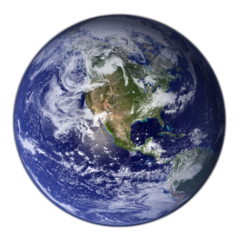
\includegraphics[width=1.8cm]{../Figure/TBP/Earth.png}};
	% Text
	\node[below, shift={(0,-0.8)}] at (earth) {$m_1$};
	\node (a) at (A) {زمین};
	
	% Moon
	\node[circle, inner sep=5.5pt, fill=black!30] (MOON) at (moon) {};
	\node[inner sep=0pt] (moon_c) at (moon) {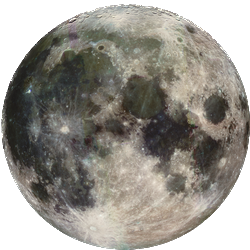
\includegraphics[width=.5cm]{../Figure/TBP/Moon.png}};
	% Text 
	\node[below, shift={(0,-0.4)}] at (MOON) {$m_2$};
	\node (b) at (B) {ماه};
	
	% Lines
	\draw[-stealth] (a) to[bend left=30] ({\r*cos(\Phi)+1},{\r*sin(\Phi)+2});
	\draw[-stealth] (b) to[bend left=-30] (MOON);
	\draw[dashed, black] (earth) -- (MOON.center);
	
	% center of mass 0.25 from earth
	\coordinate (center) at ($(earth)!0.3!(MOON)$);
	% small circle
	\draw[fill=black] (center) circle (1.5pt) node[below, shift={(0,-0.1)}] {جرم مرکز };
	
	% Calculate direction from Earth to Moon
	\pgfmathsetmacro{\xDiff}{8 - 1} % X difference between Moon and Earth
	\pgfmathsetmacro{\yDiff}{1 - 2} % Y difference between Moon and Earth
	\pgfmathsetmacro{\angle}{atan2(\yDiff,\xDiff)} % Angle of the line
	
	% Add axes at center of mass
	\draw[->, thick] (center) -- ++(\angle:2) node[above, shift={(0,0.2)}] {محور $x$};
	\draw[->, thick] (center) -- ++(\angle+90:2) node[above] {محور $y$};
	
	% add satellite with shift
	\coordinate (satellite) at ($(center)!0.5!(MOON)+(0,2)$);
	\node (satellite) at (satellite) {\faSatellite};
	
	% connect earth to satellite r1
	\draw[-stealth] (earth) -- (satellite) node[pos=0.3, above] {$\vb{r}_1$};   
	% connect moon to satellite r2
	\draw[-stealth] (MOON) -- (satellite) node[pos=0.5, above] {$\vb{r}_2$};
	% connect center of mass to satellite r
	\draw[-stealth] (center) -- (satellite) node[pos=0.5, above] {$\vb{r}$};
	% add line to show satellite is in between
	\node (c) at ($(satellite)+(1.5,0.5)$) {فضاپیما};
	\draw[-stealth] (c) to[bend left=30] (satellite);
	
\end{tikzpicture}
\caption{هندسه‌ی مسئله‌ی سه‌جسمیِ محدود در چارچوبِ چرخان}
\end{figure}



\subsection{لاگرانژ و معادلات حرکت}
با در نظر گرفتن
$G=1$
در حالت بی‌بُعد،
تابعِ لاگرانژِ جرمِ سوم در دستگاهِ چرخان برابر است با\cite{vallado2001fundamentals}
\begin{equation}\label{eq:L_crtbp}
	L=\tfrac12\bigl(\dot x^{2}+\dot y^{2}+\dot z^{2}\bigr)
	+(1-\mu)\,\frac{1}{r_{1}}+\mu\,\frac{1}{r_{2}}
	+\tfrac12\bigl(x^{2}+y^{2}\bigr),
\end{equation}
که در آن
\begin{equation}
	r_{1}=\sqrt{(x+\mu)^{2}+y^{2}+z^{2}},\qquad
	r_{2}=\sqrt{\bigl(x-1+\mu\bigr)^{2}+y^{2}+z^{2}}.
\end{equation}

با به‌کارگیری رابطه‌ی اویلر–لاگرانژ
\begin{equation*}
	\frac{\mathrm d}{\mathrm dt}\frac{\partial L}{\partial \dot q_{i}}-
	\frac{\partial L}{\partial q_{i}}=0,\qquad q_{i}\in\{x,y,z\},
\end{equation*}
معادلاتِ بی‌بُعدِ حرکتِ جرمِ سوم به دست می‌آید:
\begin{align}
	\ddot x-2\dot y &=
	x-\frac{1-\mu}{r_{1}^{3}}(x+\mu)-\frac{\mu}{r_{2}^{3}}\bigl(x-1+\mu\bigr),\\[2pt]
	\ddot y+2\dot x &=
	y-\frac{1-\mu}{r_{1}^{3}}\,y-\frac{\mu}{r_{2}^{3}}\,y,\\[2pt]
	\ddot z &= -\frac{1-\mu}{r_{1}^{3}}\,z-\frac{\mu}{r_{2}^{3}}\,z.
\end{align}
یا به نگاشتِ برداری به‌صورت زیر است.
\begin{equation}
	\ddot{\mathbf r}+2\,\boldsymbol\omega\times\dot{\mathbf r}=\nabla\Omega(\mathbf r),\qquad
	\Omega(x,y,z)=\tfrac12\bigl(x^{2}+y^{2}\bigr)+\frac{1-\mu}{r_{1}}+\frac{\mu}{r_{2}}.
\end{equation}
که در آن $\Omega$ پتانسیلِ مؤثر است و در بخش \ref{sec:lag-points} برای یافتنِ نقاطِ تعادل از شرطِ $\nabla\Omega=0$ استفاده می‌شود.
%ترم‌های کورولیس~$\pm2\,\dot{\vphantom y}$ پیامد استفاده از چارچوبِ چرخان است.


%\pgfmathsetmacro{\r}{0.8}	
%\pgfmathsetmacro{\Phi}{-160}
%\pgfmathsetmacro{\Theta}{-90}
%
%\begin{figure}[H]
%	\centering
%	\begin{tikzpicture}
%		%Grid
%		%		\draw[thin, dotted] (0,0) grid (8,8);
%		%		\foreach \i in {1,...,8}
%		%		{
%			%			\node at (\i,-2ex) {\i};	
%			%		}
%		%		\foreach \i in {1,...,8}
%		%		{
%			%			\node at (-2ex,\i) {\i};	
%			%		}
%		%		\node at (-2ex,-2ex) {0};
%		
%		% Coordinates
%		\coordinate (earth) at (1,2);
%		\coordinate (moon) at (8,1);
%		\coordinate (earth-point1) at ({\r*cos(\Theta)+1},{\r*sin(\Theta)+2});
%		\coordinate (A) at (-.5,.5);
%		\coordinate (B) at (8.5,-0.5);
%		
%		% Earth
%		\draw[thick, fill=black!30, draw=black!30
%		] (earth) circle (\r);
%		% Text
%		\node[below, shift={(0,-0.8)}] at (earth) {$m_1$};
%		\node (a) at (A) {Earth};
%		
%		% Moon
%		\node[circle, inner sep=5.5pt, fill=black!30] (MOON) at (moon) {};
%		% Text 
%		\node[below, shift={(0,-0.4)}] at (MOON) {$m_2$};
%		\node (b) at (B) {Moon};
%		
%		% Lines
%		% \draw[-latex] (earth) -- (MOON) node[pos=.55, below left] {$\vb{r}_o$};
%		% \draw[-latex] (earth) -- (earth-point1) node [pos=0.6, left] {$\vb{r}$};
%		\draw[-stealth] (a) to[bend left=30] ({\r*cos(\Phi)+1},{\r*sin(\Phi)+2});
%		\draw[-stealth] (b) to[bend left=-30] (MOON);
%		\draw[dashed, black] (earth) -- (MOON.center);
%		
%		% center of mass 0.25 from earth
%		\coordinate (center) at ($(earth)!0.3!(MOON)$);
%		% small circle
%		\draw[fill=black] (center) circle (1.5pt) node[below, shift={(0,-0.1)}] {Center of Mass};
%		% add satellite with shift
%		\coordinate (satellite) at ($(center)!0.5!(MOON)+(0,2)$);
%		% \node at ($(center)!0.5!(MOON)+(0,2)$) {\faSatellite};
%		% shift coordinate
%		\node (satellite) at (satellite) {\faSatellite};
%		
%		% connect earth to satellite r1
%		\draw[-stealth] (earth) -- (satellite) node[pos=0.5, above] {$\vb{r}_1$};   
%		% connect moon to satellite r2
%		\draw[-stealth] (MOON) -- (satellite) node[pos=0.5, above] {$\vb{r}_2$};
%		% connect center of mass to satellite r
%		\draw[-stealth] (center) -- (satellite) node[pos=0.5, above] {$\vb{r}$};
%		% add line to show satellite is in between
%		\node (c) at ($(satellite)+(1.5,0.5)$) {Satellite};
%		\draw[-stealth] (c) to[bend left=30] (satellite);
%		
%		
%		
%		
%		
%		% % Angles
%		% \pic[draw, "$\theta$", angle eccentricity=2.5, angle radius=5pt] {angle = moon--earth--earth-point1};
%		
%		% % Point
%		% \draw[fill=black] (earth) circle (1pt) node[below, shift={(0,-0.1)}] {$\mathrm{O}$};
%	\end{tikzpicture}
%	\caption{هندسه مسئله سه بدنه محدود}
%\end{figure}

%\section{نقاط لاگرانژ در مسأله‌ی سه‌جسمی محدود دایره‌ای} 
%
%
%
%\section{} نقاط تعادل (نقاط لاگرانژ $L_1$ تا $L_5$)  
%منظور از نقطه‌ی تعادل، حالتی است که جرم سوم (ذره‌ی آزمون) در دستگاه مرجع چرخان نسبت به دو جرم اصلی **ساکن** بماند. این شرایط زمانی رخ می‌دهد که سرعت و شتاب جرم سوم در دستگاه چرخان صفر شود. به‌عبارت دیگر در معادلات بالا باید $\dot{x}=\dot{y}=\dot{z}=0$ و $\ddot{x}=\ddot{y}=\ddot{z}=0$ قرار دهیم. با اعمال این شرط به معادلات لاگرانژ، مجموعه‌ای از معادلات جبری به‌دست می‌آید که مختصات نقاط تعادل (موسوم به **نقاط لاگرانژ**) را تعیین می‌کند. با قراردادن $\dot{x}=\dot{y}=0$ و $\ddot{x}=\ddot{y}=0$ در معادلات داریم:
%
%$$ 
%\begin{cases}
%	\displaystyle 0 \;=\; x \;-\; \dfrac{1-\mu}{r_1^3}(x+\mu) \;-\; \dfrac{\mu}{r_2^3}\Big(x-(1-\mu)\Big)~,  \\[2ex]
%	\displaystyle 0 \;=\; y \;-\; \dfrac{1-\mu}{r_1^3}\,y \;-\; \dfrac{\mu}{r_2^3}\,y~,  \\[1ex]
%	0 \;=\; -\,\dfrac{1-\mu}{r_1^3}\,z \;-\; \dfrac{\mu}{r_2^3}\,z~. 
%\end{cases}
%$$
%
%معادله‌ی سوم در بالا نشان می‌دهد یا باید $z=0$ باشد (نقاط تعادل همگی در صفحه‌ی حرکت هستند) یا عبارت داخل آن صفر شود که برای $z\neq0$ تنها در حالت خاصی مانند $\mu=0$ امکان‌پذیر است. بنابراین برای یافتن نقاط تعادل، حرکت جرم سوم را در همان صفحه‌ی مداری در نظر می‌گیریم ($z=0$). در این صورت $r_1$ و $r_2$ در صفحه به ترتیب $\sqrt{(x+\mu)^2+y^2}$ و $\sqrt{\big(x-(1-\mu)\big)^2+y^2}$ خواهند بود. دو معادله‌ی اول را می‌توان به صورت ساده‌تری نوشت:
%
%$$ 
%\begin{cases}
%	\displaystyle x - \dfrac{1-\mu}{r_1^3}(x+\mu) - \dfrac{\mu}{r_2^3}\Big(x-(1-\mu)\Big) = 0~,  \\[2ex]
%	\displaystyle y\,\Big[\,1 - \dfrac{1-\mu}{r_1^3} - \dfrac{\mu}{r_2^3}\Big] = 0~. 
%\end{cases}
%$$
%
%از معادله‌ی دوم نتیجه می‌شود که یا $y=0$ (نقطه‌ی تعادل روی محور $x$ واقع است) و یا پرانتز دوم صفر باشد (که منجر به رابطه‌ای بین فواصل می‌شود). بر این اساس، نقاط تعادل به دو دسته‌ی کلی تقسیم می‌شوند:
%
%- **نقاط هم‌خط (Collinear)**: این سه نقطه روی خط واصل دو جرم اصلی (محور $x$) واقع شده و بنابراین $y=0$ دارند. این نقاط را به ترتیب $L_1$، $L_2$ و $L_3$ می‌نامند.  
%- **نقاط سه‌گوش (Triangular)**: این دو نقطه در صفحه به‌صورت رئوس مثلث متساوی‌الاضلاع با دو جرم اصلی قرار می‌گیرند و دارای $y\neq0$ هستند. این دو نقطه $L_4$ و $L_5$ نام دارند.  
%
%در ادامه، هر دسته را جداگانه بررسی می‌کنیم.
%
%\section{} نقاط لاگرانژ هم‌خط ($L_1$, $L_2$, $L_3$)  
%برای نقاط واقع بر محور $x$، شرط $y=0$ را در معادلات تعادل اعمال می‌کنیم. آنگاه معادله‌ی دوم به‌طور خودکار ارضا می‌شود (زیرا $y=0$ آن را صفر می‌کند) و تنها معادله‌ی اول باقی می‌ماند:
%
%$$ 
%x - \dfrac{1-\mu}{|x+\mu|^3}(x+\mu) - \dfrac{\mu}{|x-(1-\mu)|^3}\Big(x-(1-\mu)\Big) = 0~,
%$$
%
%که در آن به علت قدرمطلق، بسته به ناحیه‌ی قرارگیری $x$، علامت عبارت‌ها مشخص می‌شود. خوشبختانه می‌توان سه ناحیه‌ی متمایز را در نظر گرفت که متناظر با سه ریشه‌ی این معادله هستند:  
%
%- **$L_1$:** بین دو جرم اصلی واقع است. در این حالت $x$ بین $-\mu$ و $1-\mu$ قرار دارد (بین موقعیت‌های جرم اول و جرم دوم). برای $L_1$ فاصله‌ی آن از جرم دوم را با $d_1$ نشان می‌دهیم (پس $x = (1-\mu) - d_1$). این فاصله را می‌توان با حل معادله‌ی بالا به‌دست آورد. معادله‌ی تعادل در این ناحیه را می‌توان پس از ساده‌سازی به صورت یک معادله‌ی درجه پنج (در $x$ یا $d_1$) نوشت که جواب تحلیلی ساده‌ای ندارد و معمولاً به روش عددی (مثلاً روش نیوتن) حل می‌شود. با این وجود، برای $\mu$های کوچک (مثلاً سیستمی مانند خورشید-زمین یا زمین-ماه) می‌توان تخمین خوبی به‌دست آورد. اگر $\mu \ll 1$ باشد (جرم دوم بسیار کوچک‌تر از جرم اول)، آنگاه $L_1$ بسیار نزدیک به جرم دوم خواهد بود و فاصله‌ی آن از جرم دوم (در واحد فاصله‌ی دو جرم اصلی) تقریباً برابر **شعاع کره‌ی هیل** جرم دوم است. شعاع هیل تقریباً $r_h \approx (\mu/3)^{1/3}$ است. بنابراین می‌توان نوشت: 
%
%$$d_1 \approx \Big(\dfrac{\mu}{3}\Big)^{1/3},$$ 
%
%و در نتیجه مختصات $L_1$ تقریباً برابر است با: 
%
%$$x_{L_1} \approx (1-\mu) - (\mu/3)^{1/3}, \qquad y_{L_1}=0.$$ 
%
%(توجه شود که برای دقت بیشتر، در صورت نیاز باید اثر $\mu$ را در قسمت $(1-\mu)$ نیز لحاظ کرد.) این فرمول یک تخمین از موقعیت $L_1$ است. در عمل حل عددی دقیق معادله، مقدار دقیق‌تری برای $x_{L_1}$ به‌دست می‌دهد. این نقطه جایی است که نیروی گرانش دو جرم (یکی کشنده به چپ و دیگری به راست) و نیروی گریز از مرکز دقیقا همدیگر را خنثی می‌کنند. 
%
%- **$L_2$:** بیرون جرم دوم (کوچک) و در امتداد همان محور قرار دارد. این نقطه در سمت راست جرم دوم واقع است ($x > 1-\mu$) و جرم دوم بین آن و جرم اول قرار می‌گیرد. اگر فاصله‌ی $L_2$ از جرم دوم را $d_2$ بگیریم ($x = (1-\mu) + d_2$)، معادله‌ی تعادل در این ناحیه نیز پس از ساده‌سازی یک معادله‌ی درجه پنج برای $d_2$ خواهد بود که باید عددی حل شود. برای $\mu$ کوچک (جرم دوم خیلی کوچک‌تر)، این فاصله نیز تقریباً برابر $(\mu/3)^{1/3}$ به‌دست می‌آید. یعنی: 
%
%$$d_2 \approx \Big(\dfrac{\mu}{3}\Big)^{1/3},$$ 
%
%و بنابراین: 
%
%$$x_{L_2} \approx (1-\mu) + (\mu/3)^{1/3}, \qquad y_{L_2}=0.$$ 
%
%این نقطه در بیرون مدار جرم دوم قرار دارد و تعادل نیروها در آن به این صورت است که نیروی گریز از مرکز به سمت بیرون توسط مجموع نیروی گرانشی دو جرم (هر دو به سمت داخل) بالانس می‌شود. 
%
%- **$L_3$:** بیرون جرم اول (بزرگ) و در امتداد خط محور $x$ در سمت مقابل جرم دوم واقع است ($x < -\mu$). این نقطه در سوی دیگر جرم بزرگ‌تر قرار دارد به‌طوری که جرم اول بین $L_3$ و جرم دوم است. برای $L_3$ نیز معادله‌ی تعادل به روش عددی حل می‌شود؛ و در حد $\mu \ll 1$ (جرم دوم بسیار کوچک)، موقعیت آن اندکی فراتر از مدار جرم اول (جرم بزرگ) است. می‌توان نشان داد برای $\mu$های بسیار کوچک: 
%
%$$x_{L_3} \approx -\,1 - \dfrac{5}{12}\,\mu, \qquad y_{L_3}=0,$$ 
%
%که نشان می‌دهد $L_3$ تقریباً به اندازه‌ی فاصله‌ی دو جرم اصلی دورتر از جرم اول است (حد $\mu \to 0$ منجر به $x=-1$ می‌شود که درست در سمت مقابل جرم دوم و هم‌فاصله با آن است) و با در نظر گرفتن جرم کوچک دوم، اندکی بیش از آن (چند صدم درصد بسته به مقدار $\mu$) فاصله می‌گیرد. به بیان دیگر، گرانش جرم دوم (هرچند کوچک) باعث می‌شود برای حفظ تعادل، جرم سومِ واقع در $L_3$ کمی به جرم بزرگ‌تر نزدیک‌تر شود تا نیروی گریز از مرکز کمتر شده و با کاهش کمی در فاصله، گرانش جرم بزرگ افزایش یابد و تعادل برقرار گردد.  
%
%معمولاً معادله‌ی دقیق مربوط به $L_1$, $L_2$ و $L_3$ را به صورت یک چندجمله‌ای درجه ۵ نسبت به متغیری کمکی بیان می‌کنند (که به **معادله‌ی کوئینتیک لاگرانژ** مشهور است) و سپس آن را با تقریب یا روش‌های عددی حل می‌نمایند. به عنوان مثال، در مراجع کلاسیک نشان داده می‌شود که اگر $\rho = x + \mu$ فاصله‌ی مرکز جرم تا نقطه‌ی تعادل در یک جهت در نظر گرفته شود، معادله‌ی درجه پنج در $\rho$ قابل بیان است. اما در کاربردهای عملی، استفاده از روش‌های عددی سریع‌تر به جواب منجر می‌شود. 
%
%\section{} نقاط لاگرانژ سه‌گوش ($L_4$, $L_5$)  
%دو نقطه‌ی تعادل دیگر در صفحه‌ی مدار به‌صورتی قرار می‌گیرند که همراه با دو جرم اصلی تشکیل یک مثلث متساوی‌الاضلاع بدهند. در چنین آرایشی، جرم سوم می‌تواند در حالت تعادل نسبی (هم‌دوران با دو جرم دیگر) باقی بماند. برای این نقاط، واضح است که $y \neq 0$ خواهد بود. بنابراین در معادلات تعادل باید قسمت داخل کروشه (که در معادله‌ی تعادل $y$ ظاهر شد) صفر گردد:
%
%$$1 - \dfrac{1-\mu}{r_1^3} - \dfrac{\mu}{r_2^3} = 0.$$
%
%این رابطه همراه با معادله‌ی تعادل در $x$ باید همزمان ارضا شوند. از آنجا که مثلث متساوی‌الاضلاع است، فاصله‌ی جرم سوم از هر دو جرم اصلی برابر است ($r_1 = r_2$). با توجه به واحد طول نرمال‌شده (فاصله‌ی بین دو جرم اصلی برابر ۱)، این فاصله باید برابر با ۱ (طول ضلع مثلث) باشد. لذا $r_1 = r_2 = 1$. در این صورت، رابطه‌ی فوق به سادگی $1 - (1-\mu) - \mu = 0$ خواهد بود که برقرار است. با استفاده از هندسه‌ی مثلث متساوی‌الاضلاع در دستگاه مختصات تعریف‌شده می‌توان مختصات دقیق $L_4$ و $L_5$ را به‌دست آورد. اگر ضلع پایینی مثلث روی محور $x$ باشد (جرم‌ها روی محور $x$ قرار دارند) و جرم سوم رأس مثلث باشد، آنگاه مختصات آن عبارت‌اند از:
%
%$$ 
%x_{L_4} \;=\; x_{L_5} \;=\; \dfrac{1}{2} - \mu~, \qquad 
%y_{L_4} \;=\; +\dfrac{\sqrt{3}}{2}~, \qquad 
%y_{L_5} \;=\; -\dfrac{\sqrt{3}}{2}~.
%$$
%
%به بیان دیگر، در دستگاه باریسنتر چرخان، هر دوی $L_4$ و $L_5$ به اندازه‌ی نیمی از فاصله‌ی دو جرم روی محور $x$ از مرکز جرم فاصله دارند (کمی جابه‌جا‌شده به سمت جرم بزرگ‌تر به اندازه‌ی $\mu$) و مؤلفه‌ی عمودی (محور $y$) آن‌ها برابر $\pm\dfrac{\sqrt{3}}{2}$ است که نشان‌دهنده‌ی زاویه‌ی $60^\circ$ نسبت به محور $x$ می‌باشد. این دو نقطه، در صورت کافی‌بودن نسبت جرم‌ها (بزرگ‌تر بودن قابل توجه جرم اول نسبت به جرم دوم؛ معمولاً $\dfrac{m_1}{m_2} > 24.96$ شرط پایداری است)، **نقاط تعادل پایدار** هستند. به عنوان مثال سیاره‌ی مشتری تعداد زیادی سیارک‌های تروجان در نقاط $L_4$ و $L_5$ خود نسبت به خورشید دارد. در مقابل، سه نقطه‌ی هم‌خط ($L_1,L_2,L_3$) پایداری ذاتی ندارند و اجسام در آن‌ها بدون تصحیح مداری معمولا از نقطه‌ی تعادل دور می‌شوند، با این حال برای تحقیقات فضایی (مانند رصدخانه‌ها یا رله‌های مخابراتی) محبوب‌اند زیرا مدارهای هاله‌ای یا لیساژور حول این نقاط با صرف انرژی اندک قابل حفظ هستند.
%
%\section{} نمونه: نقاط لاگرانژ در سیستم زمین-ماه  
%برای سیستم زمین-ماه مقدار $\mu \approx 0.01215$ است (نسبت جرم ماه به مجموع جرم زمین و ماه). در این سیستم با اعمال روابط به‌دست‌آمده می‌توان موقعیت عددی هر پنج نقطه‌ی لاگرانژ را محاسبه کرد. جدول زیر مختصات بی‌بعد (بر حسب فاصله‌ی زمین-ماه به عنوان واحد طول) این نقاط را در دستگاه مختصات تعریف‌شده‌ی باریسنتر (مرکز جرم در مبدأ، زمین در مختصات $(-\mu,0)$ و ماه در $(1-\mu,0)$) نشان می‌دهد. لازم به ذکر است که در این مقیاس، مختصات زمین تقریباً $(-0.01215,\;0)$ و ماه $(0.98785,\;0)$ می‌باشد. همان‌طور که مشاهده می‌شود، $L_1$ حدوداً در 84\% فاصله‌ی زمین-ماه (از سمت زمین) واقع شده و $L_2$ کمی بیرون مدار ماه قرار دارد. نقطه‌ی $L_3$ اندکی آن‌سوی مدار زمین (در جهت مخالف ماه) است. نقاط $L_4$ و $L_5$ نیز به‌ترتیب در بالا و پایین صفحه (در زاویه‌ی $60^\circ$) و تقریباً در فاصله‌ی مساوی از زمین و ماه قرار گرفته‌اند.
%
%| نقطه‌ی لاگرانژ | $x$ (بی‌بعد)     | $y$ (بی‌بعد)    |
%%| -------------- | -------------- | -------------- |
%%| $L_1$          | $+0.83692$     | $0$            |
%%| $L_2$          | $+1.15568$     | $0$            |
%%| $L_3$          | $-1.00506$     | $0$            |
%%| $L_4$          | $+0.48785$     | $+0.86603$     |
%%| $L_5$          | $+0.48785$     | $-0.86603$     |
%
%
%\begin{table}[H]
%	\centering
%	\caption{مقادیر عددی برای مسئله سه‌جسمی محدود (سیستم زمین-ماه)}
%\begin{tabular}{|c|c|c|}
%	\hline
%	\text{نقطه‌ی لاگرانژ} & \(x\) \, (\text{بی‌بعد}) & \(y\) \, (\text{بی‌بعد}) \\
%	\hline
%	$L_1$ & $+0.83692$ & $0$ \\
%	$L_2$ & $+1.15568$ & $0$ \\
%	$L_3$ & $-1.00506$ & $0$ \\
%	$L_4$ &$ +0.48785$ & $+0.86603$ \\
%	$L_5$ & $+0.48785$ & $-0.86603$ \\
%	\hline  
%\end{tabular}
%\end{table}
%
%
%
%
%
%
%
%
%
%\begin{figure}
%	\centering
%	\begin{tikzpicture}
%		% Define radius of the orbit
%		\def\orbitRadius{4cm}
%		
%		% Draw the orbit circle with arrows
%		\draw[-{Stealth[length=3mm]}, thick] (12:\orbitRadius) arc (12:170:\orbitRadius);
%		\draw[-{Stealth[length=3mm]}, thick] (180:\orbitRadius) arc (180:355:\orbitRadius);
%		
%		% Position for Earth (center)
%		\node[inner sep=0pt] (Earth) at (0,0) {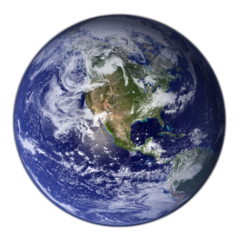
\includegraphics[width=1.8cm]{../Figure/TBP/Earth.png}};
%		\node[text=black] at (0,-1.3) {Earth};
%		
%		% Position for Moon (on the right side of the orbit)
%		\node[inner sep=0pt] (Moon) at (0.95*\orbitRadius,0) {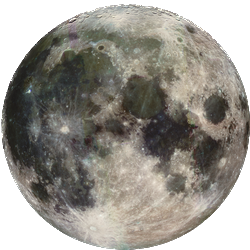
\includegraphics[width=0.6cm]{../Figure/TBP/Moon.png}};
%		\node[text=black] at (\orbitRadius,0.75) {Moon};
%		
%		% Lagrangian points
%		\coordinate (L1) at (0.8*\orbitRadius,0);
%		\coordinate (L2) at (1.2*\orbitRadius,0);
%		\coordinate (L3) at (-1*\orbitRadius,0);
%		\coordinate (L4) at (60:\orbitRadius);
%		\coordinate (L5) at (300:\orbitRadius);
%		
%		% Draw Lagrangian points as red circles
%		\foreach \point in {L1,L2,L3,L4,L5} {
%			\fill[red] (\point) circle (0.1cm);
%		}
%		
%		% Connect Lagrangian points with dashed green lines
%		\draw[dashed, blue, thick] (Earth) -- (L1);
%		\draw[dashed, blue, thick] (Moon) -- (L1);
%		\draw[dashed, blue, thick] (Moon) -- (L2);
%		\draw[dashed, blue, thick] (Earth) -- (L3);
%		\draw[dashed, blue, thick] (Earth) -- (L4);
%		\draw[dashed, blue, thick] (Moon) -- (L4);
%		\draw[dashed, blue, thick] (Earth) -- (L5);
%		\draw[dashed, blue, thick] (Moon) -- (L5);
%		
%		% Labels for the Lagrangian points
%		\node at ($(L1) + (0,0.5)$) {$L_1$};
%		\node at ($(L2) + (0,0.5)$) {$L_2$};
%		\node at ($(L3) + (0,0.5)$) {$L_3$};
%		\node at ($(L4) + (0.5,0.3)$) {$L_4$};
%		\node at ($(L5) + (0.5,-0.3)$) {$L_5$};
%	\end{tikzpicture}
%	\caption{نقاط لاگرانژ}
%\end{figure}
%
%
%
%
%
%
%
%
%
%
%
%در جدول بالا علامت مثبت/منفی $x$ نشان‌دهنده‌ی موقعیت نسبت به مرکز جرم (مبدأ مختصات) روی محور زمین-ماه است (مثبت به سمت ماه و منفی به سمت زمین) و محور $y$ عمود بر آن صفحه‌ی مداری در جهت چرخش سیستم تعریف شده است. مقادیر عددی ارائه‌شده نشان می‌دهند که در منظومه‌ی زمین-ماه، $L_1$ تقریباً در فاصله‌ی $0.84$ برابر فاصله‌ی زمین-ماه از زمین قرار دارد (یعنی فاصله‌ی آن از ماه حدود $0.16$ برابر فاصله‌ی زمین-ماه است). به طور مشابه $L_2$ حدود $1.156$ برابر فاصله‌ی زمین-ماه از زمین فاصله دارد (حدود $0.156$ برابر فاصله‌ی زمین-ماه آن‌سوی مدار ماه). نقطه $L_3$ تقریباً در فاصله‌ای برابر با فاصله‌ی زمین-ماه در سمت مقابل (پشت زمین نسبت به ماه) قرار گرفته است. نقاط $L_4$ و $L_5$ نیز تقریباً در مختصات $(0.488,\;\pm0.866)$ واقع شده‌اند که نشان‌دهنده‌ی تشکیل مثلث متساوی‌الاضلاع با زمین و ماه می‌باشد. این مقادیر و تحلیلات تأیید می‌کنند که روابط تحلیلی به‌دست‌آمده برای معادلات لاگرانژ و نقاط تعادل، به‌خوبی می‌توانند برای توصیف وضعیت‌های پایدار و ناپایدار یک جرم کوچک در میدان گرانشی دو جرم آسمانی به‌کار روند. 
%
%**مراجع:**  
%1. Richard H. Battin, *An Introduction to the Mathematics and Methods of Astrodynamics*, Revised Edition, AIAA Education Series, Eq.(1) for Lagrange’s quintic equation. (معادله درجه پنج لاگرانژ برای محاسبه نقاط $L_1, L_2, L_3$)









%--------------------------------------------------------------
\section{نقاط تعادلِ لاگرانژ}\label{sec:lag-points}

نقطه‌ی تعادل مکانی است که در چارچوبِ چرخان، جرمِ سوم بی‌حرکت بماند. این شرایط با صفرشدن مؤلفه‌های سرعت و شتاب به‌دست می‌آید؛ ازاین‌رو در معادلاتِ بالا قرار می‌دهیم $\dot x=\dot y=\dot z=\ddot x=\ddot y=\ddot z=0$. در نتیجه دستگاهِ جبریِ زیر برای مختصاتِ نقطه‌ی تعادل حاصل می‌شود:
\begin{align}
	0 &= x-\frac{1-\mu}{r_{1}^{3}}(x+\mu)-\frac{\mu}{r_{2}^{3}}\bigl(x-1+\mu\bigr),\\
	0 &= y\Bigl[1-\frac{1-\mu}{r_{1}^{3}}-\frac{\mu}{r_{2}^{3}}\Bigr],\\
	0 &= -\frac{1-\mu}{r_{1}^{3}}\,z-\frac{\mu}{r_{2}^{3}}\,z.
\end{align}
معادله‌ی سوم نشان می‌دهد برای حالت عمومی باید $z=0$ باشد؛ بنابراین نقاطِ تعادل همگی در صفحه‌ی مدار قرار می‌گیرند.

\subsubsection{دسته‌بندی کلی}
\begin{enumerate}
	\item {نقاطِ هم‌خط (\lr{Collinear}).} سه نقطه‌ی $L_{1}$، $L_{2}$ و $L_{3}$ روی خط واصلِ دو جرم قرار دارند و لذا $y=0$ است.
	\item {نقاطِ سه‌گوش (\lr{Triangular}).} دو نقطه‌ی $L_{4}$ و $L_{5}$ رأس‌های مثلثِ متساوی‌الاضلاع با دو جرمِ اصلی را تشکیل می‌دهند و در آن‌ها $y\ne0$.
\end{enumerate}



\begin{figure}[H]
	\centering
	\begin{tikzpicture}
		% Define radius of the orbit
		\def\orbitRadius{4cm}
		
		% Draw the orbit circle with arrows
		\draw[-{Stealth[length=3mm]}, thick] (12:\orbitRadius) arc (12:170:\orbitRadius);
		\draw[-{Stealth[length=3mm]}, thick] (180:\orbitRadius) arc (180:355:\orbitRadius);
		
		% Position for Earth (center)
		\node[inner sep=0pt] (Earth) at (0,0) {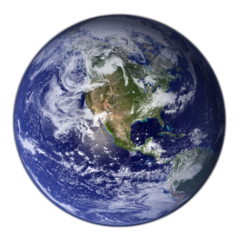
\includegraphics[width=1.8cm]{../Figure/TBP/Earth.png}};
		\node[text=black] at (0,-1.3) {Earth};
		
		% Position for Moon (on the right side of the orbit)
		\node[inner sep=0pt] (Moon) at (0.95*\orbitRadius,0) {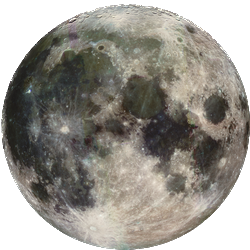
\includegraphics[width=0.6cm]{../Figure/TBP/Moon.png}};
		\node[text=black] at (\orbitRadius,0.75) {Moon};
		
		% Lagrangian points
		\coordinate (L1) at (0.8*\orbitRadius,0);
		\coordinate (L2) at (1.2*\orbitRadius,0);
		\coordinate (L3) at (-1*\orbitRadius,0);
		\coordinate (L4) at (60:\orbitRadius);
		\coordinate (L5) at (300:\orbitRadius);
		
		% Draw Lagrangian points as red circles
		\foreach \point in {L1,L2,L3,L4,L5} {
			\fill[red] (\point) circle (0.1cm);
		}
		
		% Connect Lagrangian points with dashed green lines
		\draw[dashed, blue, thick] (Earth) -- (L1);
		\draw[dashed, blue, thick] (Moon) -- (L1);
		\draw[dashed, blue, thick] (Moon) -- (L2);
		\draw[dashed, blue, thick] (Earth) -- (L3);
		\draw[dashed, blue, thick] (Earth) -- (L4);
		\draw[dashed, blue, thick] (Moon) -- (L4);
		\draw[dashed, blue, thick] (Earth) -- (L5);
		\draw[dashed, blue, thick] (Moon) -- (L5);
		
		% Labels for the Lagrangian points
		\node at ($(L1) + (0,0.5)$) {$L_1$};
		\node at ($(L2) + (0,0.5)$) {$L_2$};
		\node at ($(L3) + (0,0.5)$) {$L_3$};
		\node at ($(L4) + (0.5,0.3)$) {$L_4$};
		\node at ($(L5) + (0.5,-0.3)$) {$L_5$};
	\end{tikzpicture}
	\caption{نقاط لاگرانژ}
\end{figure}



%--------------------------------------------------------------
\subsubsection{نقاطِ هم‌خط \texorpdfstring{$(L_{1},L_{2},L_{3})$}{(L1,L2,L3)}}\label{subsec:collinear}

با اعمال $y=0$، تنها معادله‌ی زیر باقی می‌ماند
\begin{equation}\label{eq:collinear_eq}
	x-\frac{1-\mu}{|x+\mu|^{3}}(x+\mu)-\frac{\mu}{|x-1+\mu|^{3}}\bigl(x-1+\mu\bigr)=0.
\end{equation}
این معادله در سه ناحیه‌ی مجزا—بین دو جرم، بیرونِ جرمِ کوچک و بیرونِ جرمِ بزرگ—دارای یک ریشه است که به‌ترتیب نقاطِ $L_{1}$، $L_{2}$ و $L_{3}$ را تعیین می‌کند.

برای $\mu\ll1$ (همچون سامانه‌ی خورشید–زمین یا زمین–ماه) می‌توان تقریب‌های شناخته‌شده را نوشت:
\begin{align*}
	x_{L_{1}} &\simeq (1-\mu)-\bigl(\tfrac{\mu}{3}\bigr)^{1/3},\\
	x_{L_{2}} &\simeq (1-\mu)+\bigl(\tfrac{\mu}{3}\bigr)^{1/3},\\
	x_{L_{3}} &\simeq -1-\tfrac{5}{12}\,\mu; \qquad y_{L_{i}}=0.
\end{align*}
در عمل، ریشه‌ی دقیقِ معادله‌ی \eqref{eq:collinear_eq} با یک روشِ عددی (نیوتن–رافسون) محاسبه می‌شود.

%--------------------------------------------------------------
\subsubsection{نقاطِ سه‌گوش \texorpdfstring{$(L_{4},L_{5})$}{(L4,L5)}}\label{subsec:triangular}

در این نقاط $r_{1}=r_{2}=1$ و شرطِ
\(1-(1-\mu)/r_{1}^{3}-\mu/r_{2}^{3}=0\)\, به طور طبیعی برقرار است. مختصات به سادگی عبارت‌اند از
\begin{equation}
	x_{L_{4}}=x_{L_{5}}=\tfrac12-\mu,\qquad
	y_{L_{4}}=+\tfrac{\sqrt3}{2},\qquad
	y_{L_{5}}=-\tfrac{\sqrt3}{2}.
\end{equation}
پایداری این نقاط مستلزم نسبتِ جرمِ کافی است؛ شرطِ کلاسیک~$m_{1}/m_{2}>24.96$ در سامانه‌های خورشید–سیاره یا زمین–ماه به خوبی برقرار است و سببِ وجودِ خانواده‌ی سیارک‌های تروجان حول $L_{4}$ و $L_{5}$ می‌شود. در مقابل، نقاطِ هم‌خط ناپایدارند و معمولاً مأموریت‌های فضایی روی مدارهای هاله‌ای یا لیساژور در پیرامونِ آن‌ها قرار می‌گیرند.

%--------------------------------------------------------------
%\subsubsection{مثال: سامانه‌ی زمین–ماه}\label{subsec:earth-moon}

برای سامانه‌ی زمین–ماه، $\mu\simeq0.01215$ است. جدولِ زیر مختصاتِ بی‌بُعدِ هر پنج نقطه را نشان می‌دهد (واحدِ طول: فاصله‌ی زمین–ماه). موقعیتِ زمین در $(-\mu,0)$ و ماه در $(1-\mu,0)$ است.

\begin{table}[H]
	\centering
	\caption{مقادیر عددی نقاط لاگرانژ برای مسئله سه‌جسمی محدود سیستم زمین-ماه}
	\begin{tabular}{|c|c|c|}
		\hline
		\text{نقطه‌ی لاگرانژ} & \(x\) \, (\text{بی‌بعد}) & \(y\) \, (\text{بی‌بعد}) \\
		\hline
		$L_1$ & $+0.83692$ & $0$ \\
		$L_2$ & $+1.15568$ & $0$ \\
		$L_3$ & $-1.00506$ & $0$ \\
		$L_4$ &$ +0.48785$ & $+0.86603$ \\
		$L_5$ & $+0.48785$ & $-0.86603$ \\
		\hline  
	\end{tabular}
\end{table}











%\begin{table}[H]
%	\centering
%	\caption{مختصاتِ نقاطِ لاگرانژ برای سامانه‌ی زمین–ماه (مقیاسِ بی‌بُعد)}\label{tab:lagrange_earth_moon}
%	\begin{tabular}{ccc}
%		\toprule
%		\textbf{نقطه} & $x$ & $y$\\
%		\midrule
%		$L_{1}$ & $+0.83692$ & $0$\\
%		$L_{2}$ & $+1.15568$ & $0$\\
%		$L_{3}$ & $-1.00506$ & $0$\\
%		$L_{4}$ & $+0.48785$ & $+0.86603$\\
%		$L_{5}$ & $+0.48785$ & $-0.86603$\\
%		\bottomrule
%	\end{tabular}
%\end{table}
%
%\begin{figure}[H]
%	\centering
%	\begin{tikzpicture}[scale=1]
%		% orbit radius
%		\def\R{4cm}
%		
%		% orbit circle (arrowed)
%		\draw[-{Stealth[length=3mm]},thick] (12:\R) arc (12:170:\R);
%		\draw[-{Stealth[length=3mm]},thick] (180:\R) arc (180:355:\R);
%		
%		% Earth & Moon
%		\node[inner sep=0pt] (Earth) at (0,0)
%		{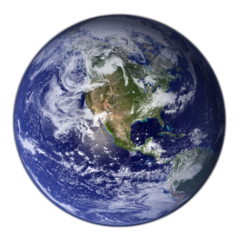
\includegraphics[width=1.8cm]{../Figure/TBP/Earth.png}};
%		\node[below=3pt of Earth] {Earth};
%		
%		\node[inner sep=0pt] (Moon) at (0.95*\R,0)
%		{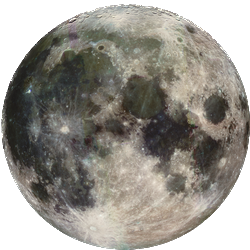
\includegraphics[width=0.6cm]{../Figure/TBP/Moon.png}};
%		\node[above right=6pt and -7pt of Moon] {Moon};
%		
%		% Lagrange coordinates
%		\coordinate (L1) at (0.8*\R,0);
%		\coordinate (L2) at (1.2*\R,0);
%		\coordinate (L3) at (-1*\R,0);
%		\coordinate (L4) at (60:\R);
%		\coordinate (L5) at (300:\R);
%		
%		% draw points
%		\foreach \P in {L1,L2,L3,L4,L5}
%		\fill[red] (\P) circle (2pt);
%		
%		% dashed helpers
%		\foreach \pair in {Earth/L1, Moon/L1, Moon/L2, Earth/L3, Earth/L4,
%			Moon/L4, Earth/L5, Moon/L5}
%		{\draw[dashed,blue] (\pair);
%		}
%		
%		% labels
%		\node[above=3pt] at (L1) {$L_1$};
%		\node[above=3pt] at (L2) {$L_2$};
%		\node[above left=2pt] at (L3) {$L_3$};
%		\node[right=4pt] at (L4) {$L_4$};
%		\node[right=4pt] at (L5) {$L_5$};
%	\end{tikzpicture}
%	\caption{جایگاه نقاطِ لاگرانژ در سامانه‌ی زمین–ماه (طرح شماتیک).}
%\end{figure}

%--------------------------------------------------------------
\noindent
این نتایج نشان می‌دهد که $L_{1}$ در حدودِ $0.84$ فاصله‌ی زمین–ماه از زمین قرار دارد (فاصله‌ی آن تا ماه در حدود $0.16$ واحد طول است) و $L_{2}$ بیرونِ مدارِ ماه است. نقطه‌ی $L_{3}$ تقریباً یک واحدِ طول در سوی مقابلِ ماه نسبت به زمین قرار دارد. دو نقطه‌ی $L_{4}$ و $L_{5}$ در مختصات $(0.488,\pm0.866)$ قرار گرفته و با زمین و ماه مثلثِ متساوی‌الاضلاع می‌سازند.

% Chapter 4: Reinforcement Learning
%\section{
%    یادگیری تقویتی
%    }
%

%--------------------------------------------------------------------
\section{یادگیری تقویتی}\label{sec:rl}

یادگیری تقویتی\LTRfootnote{Reinforcement Learning (RL)}
 شاخه‌ای از یادگیریِ ماشین است که در آن توالیِ اقدام‌ها $\boldsymbol{a}_t\in\mathcal{A}$ به‌گونه‌ای انتخاب می‌شود که بازدهِ تجمعیِ آینده بیشینه شود. یک فرایندِ تصمیم‌گیریِ مارکوف\LTRfootnote{Markov Decision Process (MDP)}
  به‌صورت $\langle\mathcal{S},\mathcal{A},p,r,\gamma\rangle$ تعریف می‌شود که در آن:
\begin{itemize}
	\item $\mathcal{S}$:
	 مجموعه‌ی حالات،
	\item $p(\boldsymbol{s}'|\boldsymbol{s},\boldsymbol{a})$:
	 دینامیکِ انتقال،
	\item $r(s,\boldsymbol{a})$:
	 پاداشِ آنی،
	\item $\gamma\in[0,1)$:
	 ضریبِ تنزیل.
\end{itemize}
\noindent
سیاست\LTRfootnote{Policy}
 $\pi(a|s)$ به‌عنوان احتمالِ انتخابِ اقدامِ $\boldsymbol{a}$ در وضعیتِ $\boldsymbol{s}$ بیان می‌شود. هدف، بیشینه‌سازیِ برگشت\LTRfootnote{Return}
 است:
 \begin{equation}
 	G_t=\sum_{k=0}^{\infty}\gamma^k r_{t+k}
 \end{equation}
 
 روش‌های \lr{RL} معمولاً در دو دسته‌ی {ارزش‌محور} (مانند \lr{Q-learning} و \lr{DQN}) و {سیاست‌محور} (مانند \lr{Reinforce}) جای می‌گیرند؛ ترکیبِ این دو به چارچوبِ \lr{Actor–Critic} منتهی می‌شود که در آن، یک بازیگر (\lr{Actor}) سیاست را به‌روزرسانی می‌کند و یک منتقد (\lr{Critic}) ارزش یا \lr{Q} برآورد می‌شود
  \cite{SuttonBarto2018}.

در حضورِ فضاهای پیوسته‌ی حالت–عمل، الگوریتم‌های  \lr{DDPG}، \lr{TD3}، \lr{SAC} و \lr{PPO} با تکیه بر شبکه‌های عصبی به‌عنوان تقریب‌گر توابع، کاراییِ بالایی نشان داده‌اند. در این پژوهش، خانواده‌ی \lr{Actor–Critic} به‌عنوان پایه‌ی توسعه‌ی کنترل‌کننده پیشنهاد شده‌ است و در ادامه، به نسخه‌ی چندعاملیِ آن در بخش~\ref{sec:marl} پیوند داده می‌شود.

% Chapter 5: Agent Simulation
\chapter{شبیه‌سازی عامل درمحیط سه جسمی}

%\begin{figure}[H]
	\centering
	\begin{tikzpicture}[x=2.4cm,y=1.2cm]
		\readlist\Nnod{4,5,5,2} % array of number of nodes per layer
		\readlist\Nstr{n,32,k} % array of string number of nodes per layer
		\readlist\Cstr{x,h^{(\prev)},u} % array of coefficient symbol per layer
		\def\yshift{0.55} % shift last node for dots
		% LOOP over LAYERS
		% LOOP over LAYERS
		\foreachitem \N \in \Nnod{
			\def\lay{\Ncnt} % alias of index of current layer
			\pgfmathsetmacro\prev{int(\Ncnt-1)} % number of previous layer
			\foreach \i [evaluate={\c=int(\i==\N);
				\layercheck=\ifnum\Ncnt=1 0 \else \ifnum\Ncnt=\Nnodlen 0 \else \yshift \fi \fi;
				\y=\N/2-\i*1.2-\c*\layercheck;
				\x=\lay; \n=\nstyle;
				\index=(\i<\N?int(\i):"\Nstr[\n]");}] in {1,...,\N}{ % loop over nodes
				% NODES
				\ifnum \lay=1
				\ifnum \i=1
				\node[node \n] (N\lay-\i) at (\x,\y) {$\delta x$};
				\fi
				\ifnum \i=2
				\node[node \n] (N\lay-\i) at (\x,\y) {$\delta y$};
				\fi
				\ifnum \i=3
				\node[node \n] (N\lay-\i) at (\x,\y) {$\delta {\dot{x}}$};
				\fi
				\ifnum \i=4
				\node[node \n] (N\lay-\i) at (\x,\y) {$\delta {\dot{y}}$};
				\fi
				\else \ifnum \lay=\Nnodlen
				\ifnum \i=1
				\node[node \n] (N\lay-\i) at (\x,\y) {$u_x$};
				\fi
				\ifnum \i=2
				\node[node \n] (N\lay-\i) at (\x,\y) {$u_y$};
				\fi
				\else
				\node[node \n] (N\lay-\i) at (\x,\y) {$\strut\Cstr[\n]_{\index}$};
				\fi \fi
				% CONNECTIONS
				\ifnumcomp{\lay}{>}{1}{ % connect to previous layer
					\foreach \j in {1,...,\Nnod[\prev]}{ % loop over nodes in previous layer
						\draw[white,line width=1.2,shorten >=1] (N\prev-\j) -- (N\lay-\i);
						\draw[connect] (N\prev-\j) -- (N\lay-\i);
					}
					%   \ifnum \lay=\Nnodlen
					%     \draw[connect] (N\lay-\i) --++ (0.5,0); % arrows out
					%   \fi
				}{
					%   \draw[connect] (0.5,\y) -- (N\lay-\i); % arrows in
				}
			}
			% Dots (skip first and last layers)
			\ifnum \lay>1 \ifnum \lay<\Nnodlen
			\path (N\lay-\N) --++ (0,1+\yshift) node[midway,scale=1.6] {$\vdots$}; % dots
			\fi \fi
		}
		% LABELS
		\node[above=.1,align=center,mydarkgreen] at (N1-1.90) {{لایه}\\[-0.6em]{ورودی}};
		\node[above=.1,align=center,mydarkblue] at (N2-1.90) {{لایه}\\[-0.6em]{پنهان}};
		\node[above=.1,align=center,mydarkblue] at (N3-1.90) {{لایه}\\[-0.6em]{پنهان}};
		\node[above=.1,align=center,mydarkred] at (N\Nnodlen-1.90) {{لایه}\\[-0.6em]{خروجی}};
	\end{tikzpicture}
	\caption{ساختار شبکه عصبی سیاست}
	\label{fig:actor_nn}
\end{figure}
	

	
		در این فصل، فرآیند شبیه‌سازی عامل هوشمند کنترل‌کننده فضاپیما در محیط دینامیکی سه جسمی بررسی شده است.
		در بخش \ref{sec:agent_design}
		به
		طراحی و 
		در بخش 
		\ref{sec:agent_sim}
	به	شبیه‌سازی عامل هدایت‌کننده مبتنی بر یادگیری تقویتی است
		پرداخته شده است. این عامل طراحی و شبیه‌سازی شده باید توانایی این را داشته باشد 
		 که  فضاپیما را به‌طور مؤثر به سمت اهداف تعیین‌شده هدایت کند، در حالی که محدودیت‌هایی نظیر مصرف سوخت و وجود اغتشاش دارد.
	
	
	\section{طراحی عامل}\label{sec:agent_design}
	
	در این زیربخش، معماری عامل هوشمند کنترل‌کننده فضاپیما در محیط سه جسمی شرح داده شده است. این معماری شامل تعریف عامل، فضای حالت و عمل، و تابع پاداش است.

	
	\subsection{ فضای حالت}

فضای حالت\LTRfootnote{State Space}
در این پژوهش به‌گونه‌ای طراحی شده است که وضعیت دینامیکی فضاپیما را نسبت به یک مسیر و سرعت مرجع مشخص می‌کند. این فضا شامل اختلاف‌های موقعیت و سرعت از مسیر و سرعت مرجع  است و به‌صورت زیر تعریف می‌شود:
\[
S = \{ \delta x, \delta y, \delta \dot{x}, \delta \dot{y} \}
\]

که در آن:
\begin{itemize}
    \item \( \delta x, \delta y \): اختلاف موقعیت فضاپیما نسبت به مسیر مرجع در محورهای \( x, y \) .
    \item \( \delta \dot{x}, \delta \dot{y} \): اختلاف سرعت فضاپیما نسبت به سرعت مرجع در محورهای \( x, y \) .
\end{itemize}

هر یک از این متغیرها به‌طور مستقل وضعیت فضاپیما را در یک جهت خاص توصیف می‌کنند و امکان تحلیل دقیق انحرافات را فراهم می‌سازند.
%\subsection{دلیل انتخاب اختلاف‌ها به‌عنوان متغیرهای فضای حالت}
استفاده از اختلاف‌های موقعیت و سرعت به جای مقادیر مطلق، به دلایل زیر انجام شده است:
\begin{itemize}
    \item \textbf{تمرکز بر انحرافات}: هدف اصلی سیستم کنترلی، کاهش انحرافات از مسیر و سرعت مطلوب است. با استفاده از اختلاف‌ها، کنترلر می‌تواند به طور مستقیم بر این انحرافات اثر بگذارد و نیازی به محاسبه مقادیر مطلق موقعیت و سرعت ندارد.
%    \item \textbf{سادگی در طراحی کنترلر}: تعریف فضای حالت بر اساس اختلاف‌ها، معادلات دینامیکی را ساده‌تر می‌کند و طراحی کنترلرهای خطی یا غیرخطی را تسهیل می‌نماید.
%    \item \textbf{بهینه‌سازی محاسبات}: از آنجایی که مسیر و سرعت مرجع معمولاً ثابت یا از پیش تعیین‌شده هستند، محاسبه اختلاف‌ها به جای مقادیر مطلق، حجم محاسبات را کاهش می‌دهد و دقت شبیه‌سازی را افزایش می‌دهد.
    \item \textbf{سازگاری با یادگیری تقویتی}: در الگوریتم‌های یادگیری تقویتی، فضاهای حالت مبتنی بر اختلاف معمولاً دامنه محدودتری دارند که فرآیند یادگیری را سریع‌تر و پایدارتر می‌کند.
\end{itemize}

	
	\subsection{فضای عمل }
	

	
		فضای عمل\LTRfootnote{Action Space} 
		فضاپیما با پیشران‌کم
		مجموعه‌ای از عمل‌های پیوسته است که فضاپیما می‌تواند در محیط شبیه‌سازی انجام دهد. این فضا به‌گونه‌ای طراحی شده که امکان اعمال نیرو در جهت‌های مشخص و با مقادیر متناسب با توان واقعی فضاپیماها فراهم شود. به‌طور خاص، فضای اقدام شامل موارد زیر است:
	
	\begin{itemize}
		\item \textbf{نیروی اعمال‌شده در جهت \( x \)}: این متغیر پیوسته، مقدار نیرویی را که در جهت محور \( x \) به فضاپیما وارد می‌شود، تعیین می‌کند. دامنه این نیرو بر اساس توان پیشرانه‌های موجود در فضاپیماهای واقعی انتخاب شده است. به عبارت دیگر، اگر حداکثر نیروی قابل اعمال در جهت \( x \) برابر با \( f_{x,\max} \) باشد، این متغیر می‌تواند مقادیری در بازه \( [-f_{x,\max}, f_{x,\max}] \) داشته باشد.
		
		\item \textbf{نیروی اعمال‌شده در جهت \( y \)}: این متغیر پیوسته، مقدار نیرویی را که در جهت محور \( y \) به فضاپیما وارد می‌شود، مشخص می‌کند. مشابه جهت \( x \)، دامنه این نیرو نیز بر اساس توان پیشرانه‌های موجود تعیین شده و می‌تواند در بازه \( [-f_{y,\max}, f_{y,\max}] \) قرار گیرد.
	\end{itemize}
	
	انتخاب این نیروها بر اساس ویژگی‌های واقعی فضاپیماها، به‌ویژه توان و محدودیت‌های پیشرانه‌های آن‌ها، صورت گرفته است. این امر اطمینان می‌دهد که شبیه‌سازی تا حد ممکن به شرایط واقعی نزدیک باشد و نتایج به‌دست‌آمده قابلیت تعمیم به کاربردهای عملی را داشته باشند. همچنین، تعریف فضای اقدام به‌صورت پیوسته، امکان کنترل دقیق و انعطاف‌پذیر بر حرکت فضاپیما را فراهم می‌کند، که برای دستیابی به اهداف کنترلی در محیط‌های دینامیکی پیچیده ضروری است.
	به‌طور خلاصه، فضای اقدام به‌صورت زیر تعریف می‌شود:
	\[
	a = \{ f_x, f_y \mid f_x \in [-f_{x,\max}, f_{x,\max}], \, f_y \in [-f_{y,\max}, f_{y,\max}] \}
	\]
	
	
	
	
	
	
	
	
	
	
	
	
	
	
	
	\subsection{تابع پاداش }
	تابع پاداش\LTRfootnote{Reward Function}
 به‌منظور هدایت رفتار عامل طراحی شده و شامل دو مؤلفه اصلی است:
	\begin{itemize}
		\item \textbf{پاداش برای دستیابی به هدف}: تشویق عامل برای نزدیک شدن به مدار هدف.
		\item \textbf{جریمه برای مصرف سوخت}: تنبیه برای استفاده بیش از حد از پیشرانه.
		\item \textbf{جریمه برای انحراف از مسیر مرجع}: تنبیه برای خروج از مسیر مرجع.
	\end{itemize}
	تابع پاداش به‌صورت زیر تعریف می‌شود:
	\[
	r(s, a) = r_{\text{target}}(s) + r_{\text{thrust}}(a)  + r_{\text{divergence}}(s)
	\]
	که در آن مؤلفه‌های تابع پاداش به‌صورت زیر تعریف شده‌اند:
	\begin{align}
	r_{\text{target}}(s) &= -k_1 \cdot d(s, s_{\text{target}}) \\
	r_{\text{thrust}}(a) &= -k_2 \cdot \|a\| \\	
	r_{\text{divergence}}(s) &= \begin{cases}
	-k_3 & \text{if} ~ d(s, s_{\text{reference}}) > \epsilon \\
	0 & \text{otherwise}
	\end{cases}
	\end{align}
تابع \( d(s, s') \) فاصله بین دو وضعیت \( s \) و \( s' \) را نشان می‌دهد که معمولاً به‌صورت فاصله اقلیدسی محاسبه می‌شود.
ضرایب \( k_1, k_2, k_3 \) از طریق آزمایش و خطا تنظیم شده‌اند تا تعادل مناسبی بین دستیابی به هدف، بهینه‌سازی مصرف سوخت، و حفظ مسیر مرجع برقرار شود. علاوه بر این، این ضرایب تأثیر مستقیمی بر پایداری و فرآیند یادگیری عامل دارند. به‌عنوان مثال، انتخاب مقادیر بیش از حد بزرگ برای \( k_1 \) ممکن است باعث شود عامل به‌سرعت به سمت هدف حرکت کند اما پایداری مسیر را از دست بدهد، در حالی که مقادیر بزرگ \( k_3 \) می‌تواند عامل را بیش از حد محافظه‌کار کرده و فرآیند یادگیری را کند نماید. تنظیم دقیق این ضرایب، نه‌تنها عملکرد عامل را بهینه می‌کند، بلکه پایداری عددی و سرعت همگرایی الگوریتم یادگیری تقویتی را نیز تضمین می‌نماید.
	
	
	
	
	
	
	
	
	
	
	
	
	
	
	
	
	
	
	
	
	
	
	
	
	
	
	\section{شبیه‌سازی عامل}\label{sec:agent_sim}
	
	در این زیربخش، فرآیند شبیه‌سازی و آموزش عامل با استفاده از الگوریتم‌های یادگیری تقویتی پیشرفته شرح داده می‌شود. الگوریتم‌های مورد استفاده، مراحل آموزش، و نتایج حاصل از شبیه‌سازی ارائه می‌گردند.
	
	\subsection{الگوریتم‌های مورد استفاده}
	
	برای آموزش عامل، الگوریتم‌های زیر به‌کار گرفته شده‌اند:
	
	\begin{table}[h]
		\centering
		\caption{ویژگی‌های الگوریتم‌های مورد استفاده در شبیه‌سازی}
		\begin{tabular}{|c|c|c|c|c|c|}
			\hline
			\multirow{2}{*}{\textbf{الگوریتم}} & \multicolumn{2}{c|}{\textbf{شبکه \lr{Actor}}} & \multicolumn{2}{c|}{\textbf{شبکه \lr{Critic}}} & \multirow{2}{*}{\textbf{تعداد پارامترها}} \\
			\cline{2-5}
			& \textbf{لایه‌ها} & \textbf{نودها} & \textbf{لایه‌ها} & \textbf{نودها} & \\
			\hline
			\lr{DDPG} & \(3\) & \( (2^8, 2^7, 2^6) \) & \(3\) & \( (2^8, 2^7, 2^6) \) & \(150 \times 10^3\) \\
			\hline
			\lr{PPO} & \(2\) & \( (2^7, 2^6) \) & \(2\) & \( (2^7, 2^6) \) & \(50 \times 10^3\) \\
			\hline
			\lr{SAC} & \(3\) & \( (2^8, 2^7, 2^6) \) & \(3\) & \( (2^8, 2^7, 2^6) \) & \(160 \times 10^3\) \\
			\hline
			\lr{TD3} & \(3\) & \( (2^8, 2^7, 2^6) \) & \(4\) & \( (2^8, 2^7, 2^7, 2^6) \) & \(200 \times 10^3\) \\
			\hline
		\end{tabular}
	\end{table}
	این الگوریتم‌ها به دلیل توانایی در مدیریت فضاهای پیوسته و عملکرد مؤثر در محیط‌های پیچیده انتخاب شده‌اند.
	در شکل
	\ref{fig:actor_nn}
	شبکه عصبی شبیه‌سازی شده آورده شده است.
	\begin{figure}[H]
	\centering
	\begin{tikzpicture}[x=2.4cm,y=1.2cm]
		\readlist\Nnod{4,5,5,2} % array of number of nodes per layer
		\readlist\Nstr{n,32,k} % array of string number of nodes per layer
		\readlist\Cstr{x,h^{(\prev)},u} % array of coefficient symbol per layer
		\def\yshift{0.55} % shift last node for dots
		% LOOP over LAYERS
		% LOOP over LAYERS
		\foreachitem \N \in \Nnod{
			\def\lay{\Ncnt} % alias of index of current layer
			\pgfmathsetmacro\prev{int(\Ncnt-1)} % number of previous layer
			\foreach \i [evaluate={\c=int(\i==\N);
				\layercheck=\ifnum\Ncnt=1 0 \else \ifnum\Ncnt=\Nnodlen 0 \else \yshift \fi \fi;
				\y=\N/2-\i*1.2-\c*\layercheck;
				\x=\lay; \n=\nstyle;
				\index=(\i<\N?int(\i):"\Nstr[\n]");}] in {1,...,\N}{ % loop over nodes
				% NODES
				\ifnum \lay=1
				\ifnum \i=1
				\node[node \n] (N\lay-\i) at (\x,\y) {$\delta x$};
				\fi
				\ifnum \i=2
				\node[node \n] (N\lay-\i) at (\x,\y) {$\delta y$};
				\fi
				\ifnum \i=3
				\node[node \n] (N\lay-\i) at (\x,\y) {$\delta {\dot{x}}$};
				\fi
				\ifnum \i=4
				\node[node \n] (N\lay-\i) at (\x,\y) {$\delta {\dot{y}}$};
				\fi
				\else \ifnum \lay=\Nnodlen
				\ifnum \i=1
				\node[node \n] (N\lay-\i) at (\x,\y) {$u_x$};
				\fi
				\ifnum \i=2
				\node[node \n] (N\lay-\i) at (\x,\y) {$u_y$};
				\fi
				\else
				\node[node \n] (N\lay-\i) at (\x,\y) {$\strut\Cstr[\n]_{\index}$};
				\fi \fi
				% CONNECTIONS
				\ifnumcomp{\lay}{>}{1}{ % connect to previous layer
					\foreach \j in {1,...,\Nnod[\prev]}{ % loop over nodes in previous layer
						\draw[white,line width=1.2,shorten >=1] (N\prev-\j) -- (N\lay-\i);
						\draw[connect] (N\prev-\j) -- (N\lay-\i);
					}
					%   \ifnum \lay=\Nnodlen
					%     \draw[connect] (N\lay-\i) --++ (0.5,0); % arrows out
					%   \fi
				}{
					%   \draw[connect] (0.5,\y) -- (N\lay-\i); % arrows in
				}
			}
			% Dots (skip first and last layers)
			\ifnum \lay>1 \ifnum \lay<\Nnodlen
			\path (N\lay-\N) --++ (0,1+\yshift) node[midway,scale=1.6] {$\vdots$}; % dots
			\fi \fi
		}
		% LABELS
		\node[above=.1,align=center,mydarkgreen] at (N1-1.90) {{لایه}\\[-0.6em]{ورودی}};
		\node[above=.1,align=center,mydarkblue] at (N2-1.90) {{لایه}\\[-0.6em]{پنهان}};
		\node[above=.1,align=center,mydarkblue] at (N3-1.90) {{لایه}\\[-0.6em]{پنهان}};
		\node[above=.1,align=center,mydarkred] at (N\Nnodlen-1.90) {{لایه}\\[-0.6em]{خروجی}};
	\end{tikzpicture}
	\caption{ساختار شبکه عصبی سیاست}
	\label{fig:actor_nn}
\end{figure}
	\begin{figure}[H]
	\centering
\begin{tikzpicture}[x=2.8cm,y=1.5cm]
	\readlist\Nnod{6,7,7,1} % array of number of nodes per layer
	\readlist\Nstr{n,32,k} % array of string number of nodes per layer
	\readlist\Cstr{x,h^{(\prev)},u} % array of coefficient symbol per layer
	\def\yshift{0.55} % shift last node for dots
	
	% LOOP over LAYERS
	% LOOP over LAYERS
	\foreachitem \N \in \Nnod{
		\def\lay{\Ncnt} % alias of index of current layer
		\pgfmathsetmacro\prev{int(\Ncnt-1)} % number of previous layer
		\foreach \i [evaluate={\c=int(\i==\N); 
			\layercheck=\ifnum\Ncnt=1 0 \else \ifnum\Ncnt=\Nnodlen 0 \else \yshift \fi \fi;
			\y=\N/2-\i-\c*\layercheck;
			\x=\lay; \n=\nstyle;
			\index=(\i<\N?int(\i):"\Nstr[\n]");}] in {1,...,\N}{ % loop over nodes
			% NODES
			\ifnum \lay=1
			\ifnum \i=1
			\node[node \n] (N\lay-\i) at (\x,\y) {$\delta x$};
			\fi
			\ifnum \i=2
			\node[node \n] (N\lay-\i) at (\x,\y) {$\delta y$};
			\fi
			\ifnum \i=3
			\node[node \n] (N\lay-\i) at (\x,\y) {$\delta {\dot{x}}$};
			\fi
			\ifnum \i=4
			\node[node \n] (N\lay-\i) at (\x,\y) {$\delta {\dot{y}}$};
			\fi
			\ifnum \i=5
			\node[node \n] (N\lay-\i) at (\x,\y) {$u_x$};
			\fi
			\ifnum \i=6
			\node[node \n] (N\lay-\i) at (\x,\y) {$u_y$};
			\fi
			\else \ifnum \lay=\Nnodlen
			\ifnum \i=1
			\node[node \n] (N\lay-\i) at (\x,\y) {$Q$};
			\fi
			\ifnum \i=2
			\node[node \n] (N\lay-\i) at (\x,\y) {$u_y$};
			\fi
			\else
			\node[node \n] (N\lay-\i) at (\x,\y) {$\strut\Cstr[\n]_{\index}$};
			\fi \fi
			% CONNECTIONS
			\ifnumcomp{\lay}{>}{1}{ % connect to previous layer
				\foreach \j in {1,...,\Nnod[\prev]}{ % loop over nodes in previous layer
					\draw[white,line width=1.2,shorten >=1] (N\prev-\j) -- (N\lay-\i);
					\draw[connect] (N\prev-\j) -- (N\lay-\i);
				}
				%   \ifnum \lay=\Nnodlen
				%     \draw[connect] (N\lay-\i) --++ (0.5,0); % arrows out
				%   \fi
			}{
				%   \draw[connect] (0.5,\y) -- (N\lay-\i); % arrows in
			}
		}
		
		% Dots (skip first and last layers)
		\ifnum \lay>1 \ifnum \lay<\Nnodlen
		\path (N\lay-\N) --++ (0,1+\yshift) node[midway,scale=1.6] {$\vdots$}; % dots
		\fi \fi
	}
	
	
	
	% LABELS
	\node[above=.1,align=center,mydarkgreen] at (N1-1.90) {\lr{Input}\\[-0.6em]\lr{layer}};
	\node[above=.1,align=center,mydarkblue] at (N2-1.90) {\lr{Hidden}\\[-0.6em]\lr{layers}};
	\node[above=.1,align=center,mydarkblue] at (N3-1.90) {\lr{Hidden}\\[-0.6em]\lr{layers}};
	\node[above=.1,align=center,mydarkred] at (N\Nnodlen-1.90) {\lr{Output}\\[-0.6em]\lr{layer}};
\end{tikzpicture}
	\caption{ساختار شبکه عصبی نقاد}
	\label{fig:actor_nn}
\end{figure}

\subsection{فرآیند آموزش}

آموزش عامل به‌صورت کلی در چند مرحله انجام شده است. ابتدا، کاوش اولیه در محیط با استفاده از یک سیاست تصادفی صورت گرفته و تجربه‌های اولیه جمع‌آوری شده‌اند. سپس، شبکه‌های عصبی الگوریتم‌ها با بهره‌گیری از این تجربه‌ها به‌روزرسانی شده‌اند. در نهایت، پارامترهای کلیدی مانند نرخ یادگیری و اندازه بافر تجربه تنظیم شده‌اند تا پایداری فرآیند تضمین شود.

برای پیاده‌سازی این فرآیند، از چارچوب \lr{PyTorch} استفاده شده است. همچنین، به‌منظور جلوگیری از بیش‌برازش، تکنیک \lr{Noise Exploration} به‌کار گرفته شده است. آموزش تا زمانی ادامه یافته که موفقیت عامل در بیش از 90 درصد موارد به‌دست آمده باشد. در این راستا، برای بهینه‌سازی پارامترهای شبکه‌های عصبی، از روش \lr{Backpropagation} استفاده شده است. این روش بر اساس گرادیان تابع خطا نسبت به پارامترها عمل می‌کند که به‌صورت زیر بیان می‌شود:

\begin{equation}
	\frac{\partial L}{\partial w} = \frac{\partial L}{\partial y} \cdot \frac{\partial y}{\partial w}
\end{equation}
%که در آن:
که در آن \( L \) تابع خطا، \( w \) وزن‌های شبکه، و \( y \) خروجی شبکه عصبی است. 
%\begin{itemize}
%	\item \( L \): تابع خطا (Loss Function) است که معمولاً به‌صورت \( L = \mathbb{E}[(r - \hat{r})^2] \) تعریف می‌شود.
%	\item \( w \): پارامترهای شبکه (وزن‌ها).
%	\item \( y \): خروجی شبکه عصبی.
%\end{itemize}
به‌روزرسانی وزن‌ها با استفاده از روش گرادیان نزولی انجام شده است:
\begin{equation}
	w_{t+1} = w_t - \eta \cdot \frac{\partial L}{\partial w}
\end{equation}
که \( \eta \) نرخ یادگیری است و به‌عنوان یک پارامتر کلیدی تنظیم شده است.





% Chapter 6: Multi-Agent Reinforcement Learning
\chapter{یادگیری تقویتی چند عاملی}
کاربردهای پیچیده در یادگیری تقویتی نیازمند اضافه کردن چندین عامل\LTRfootnote{Multi-Agent} برای انجام همزمان وظایف مختلف هستند.
با این حال، افزایش تعداد عامل‌ها چالش‌هایی در مدیریت تعاملات میان آن‌ها به همراه دارد.
در این فصل، بر اساس مسئله بهینه‌سازی برای هر عامل، مفهوم تعادل\LTRfootnote{Equilibrium} معرفی شده تا رفتارهای توزیعی چندعاملی را تنظیم کند.
رابطه رقابت میان عامل‌ها در سناریوهای مختلف تحلیل شده و آن‌ها با الگوریتم‌های معمول یادگیری تقویتی چندعاملی ترکیب شده‌اند. بر اساس انواع تعاملات، یک چارچوب نظریه بازی برای مدل‌سازی عمومی در سناریوهای چندعاملی استفاده شده است. با تحلیل بهینه‌سازی و وضعیت تعادل برای هر بخش از چارچوب، سیاست بهینه یادگیری تقویتی چندعاملی برای هر عامل بررسی شده است.




  \section{تعاریف و مفاهیم اساسی }
یادگیری تقویتی چندعاملی\LTRfootnote{Multi-Agent Reinforcement Learning (MARL)} به بررسی چگونگی یادگیری و تصمیم‌گیری چندین عامل مستقل در یک محیط مشترک پرداخته می‌شود. برای تحلیل دقیق و درک بهتر این حوزه، اجزای اصلی آن شامل عامل، سیاست و مطلوبیت\LTRfootnote{Utility} در نظر گرفته می‌شوند که در ادامه به صورت مختصر و منسجم تشریح می‌گردند.

\begin{itemize}
	\item عامل: یک موجودیت مستقل به عنوان عامل تعریف می‌شود که به صورت خودمختار با محیط تعامل کرده و بر اساس مشاهدات رفتار سایر عامل‌ها، سیاست‌هایش انتخاب می‌گردند تا سود حداکثر یا ضرر حداقل حاصل شود. در سناریوهای مورد بررسی، چندین عامل به صورت مستقل عمل می‌کنند؛ اما اگر تعداد عامل‌ها به یک کاهش یابد، \lr{MARL} به یادگیری تقویتی معمولی تبدیل می‌شود.
	
	\item سیاست: برای هر عامل در \lr{MARL}، سیاستی خاص در نظر گرفته می‌شود که به عنوان روشی برای انتخاب اقدامات بر اساس وضعیت محیط و رفتار سایر عامل‌ها تعریف می‌گردد. این سیاست‌ها با هدف به حداکثر رساندن سود و به حداقل رساندن هزینه طراحی شده و تحت تأثیر محیط و سیاست‌های دیگر عامل‌ها قرار می‌گیرند.
	
	\item مطلوبیت: مطلوبیت
	هر عامل بر اساس نیازها و وابستگی‌هایش به محیط و سایر عامل‌ها تعریف شده و به صورت سود منهای هزینه، با توجه به اهداف مختلف محاسبه می‌شود. در سناریوهای چندعاملی، از طریق یادگیری از محیط و تعامل با دیگران، مطلوبیت هر عامل بهینه می‌گردد.
\end{itemize}

در این چارچوب، برای هر عامل در \lr{MARL} تابع مطلوبیت خاصی در نظر گرفته شده و بر اساس مشاهدات و تجربیات حاصل از تعاملات، یادگیری سیاست به صورت مستقل انجام می‌شود تا ارزش مطلوبیت به حداکثر برسد، بدون اینکه مستقیماً به مطلوبیت سایر عامل‌ها توجه شود. این فرآیند ممکن است به رقابت یا همکاری میان عامل‌ها منجر گردد.
 با توجه به پیچیدگی تعاملات میان چندین عامل، تحلیل نظریه بازی‌ها به عنوان ابزاری مؤثر برای تصمیم‌گیری در این حوزه به کار گرفته می‌شود. بسته به سناریوهای مختلف، این بازی‌ها در دسته‌بندی‌های متفاوتی قرار داده شده که در بخش‌های بعدی بررسی خواهند شد.

  % \section{اهمیت یادگیری تقویتی چندعاملی}

یادگیری تقویتی چندعاملی به دلیل قابلیت‌های بالقوه‌اش در مدل‌سازی و حل مسائل پیچیده و پویا، اهمیت زیادی در حوزه‌های مختلف علمی و صنعتی دارد. در این بخش، به بررسی اهمیت \lr{MARL} در زمینه‌های مختلف پرداخته و نقش آن را در توسعه سیستم‌های هوشمند متعدد بررسی می‌کنیم.

\subsubsection{مدل‌سازی سیستم‌های پیچیده و پویا}
یکی از دلایل اصلی اهمیت \lr{MARL}، توانایی آن در مدل‌سازی سیستم‌های پیچیده و پویا است. در بسیاری از کاربردهای واقعی، سیستم‌ها شامل چندین عامل هستند که به صورت همزمان و مستقل به تعامل می‌پردازند. به عنوان مثال، در شبکه‌های ترافیکی، هر خودرو می‌تواند به عنوان یک عامل مستقل عمل کند که نیاز به هماهنگی و تعامل با سایر خودروها برای بهینه‌سازی جریان ترافیک دارد. \lr{MARL} با فراهم کردن چارچوبی برای تعامل و یادگیری میان این عوامل، امکان بهبود کارایی و کاهش ترافیک را فراهم می‌کند.

\subsubsection{کاربرد در رباتیک چندعاملی}
در حوزه رباتیک، سیستم‌های چندعاملی می‌توانند برای انجام وظایف پیچیده‌ای مانند جست‌وجو و نجات، حمل و نقل مواد، و عملیات هماهنگ در محیط‌های غیرقابل پیش‌بینی مورد استفاده قرار گیرند. به عنوان مثال، گروهی از ربات‌های پرنده (دُرون‌ها) می‌توانند با همکاری و تبادل اطلاعات، منطقه‌ای وسیع را برای شناسایی اهداف نظارت کنند یا به سرعت به تغییرات محیطی واکنش نشان دهند. \lr{MARL} در این زمینه بهبود هماهنگی میان ربات‌ها و افزایش کارایی عملیات‌های چندعاملی را ممکن می‌سازد.

\subsubsection{مدیریت منابع در شبکه‌های ارتباطی}
شبکه‌های ارتباطی مدرن نیازمند مدیریت بهینه منابع مانند پهنای باند، انرژی و ظرفیت ذخیره‌سازی هستند. در این راستا، \lr{MARL} می‌تواند به عنوان یک ابزار قدرتمند برای تخصیص بهینه منابع به عوامل مختلف شبکه عمل کند. به عنوان مثال، در شبکه‌های بی‌سیم، هر دستگاه کاربر می‌تواند به عنوان یک عامل مستقل عمل کرده و با یادگیری و تعامل با سایر دستگاه‌ها، نحوه بهینه‌سازی مصرف انرژی و پهنای باند را پیدا کند. این امر منجر به افزایش کارایی شبکه و کاهش هزینه‌های عملیاتی می‌شود.

\subsubsection{توسعه الگوریتم‌های پیشرفته‌تر و قابل اعتمادتر}
یکی دیگر از جنبه‌های مهم \lr{MARL}، فهم و تحلیل تعاملات میان عوامل مختلف است که می‌تواند به توسعه الگوریتم‌های پیشرفته‌تر و قابل اعتمادتر منجر شود. با مطالعه رفتارها و استراتژی‌های مختلف در محیط‌های چندعاملی، پژوهشگران قادر به طراحی الگوریتم‌هایی می‌شوند که نه تنها بهینه عمل می‌کنند بلکه مقاومت بالایی در برابر تغییرات محیطی و رفتارهای غیرمنتظره دارند. این الگوریتم‌ها می‌توانند در شرایط متنوع و پیچیده‌تر به خوبی عمل کنند و از خطاها و ناهنجاری‌های احتمالی جلوگیری نمایند.

\subsubsection{کاربرد در بازی‌های چندعاملی و شبیه‌سازی‌های اقتصادی}
بازی‌های چندعاملی و شبیه‌سازی‌های اقتصادی از دیگر حوزه‌هایی هستند که به شدت از \lr{MARL} بهره‌مند می‌شوند. در بازی‌های استراتژیک چند نفره، \lr{MARL} می‌تواند به بازیگران کمک کند تا استراتژی‌های بهینه‌ای برای رقابت و همکاری با یکدیگر توسعه دهند. همچنین، در شبیه‌سازی‌های اقتصادی، \lr{MARL} می‌تواند به مدل‌سازی و تحلیل رفتارهای بازار و تصمیم‌گیری‌های اقتصادی کمک کند، که این امر به پیش‌بینی دقیق‌تر روندهای اقتصادی و بهبود سیاست‌گذاری‌های مالی منجر می‌شود.

\subsubsection{افزایش قابلیت انعطاف‌پذیری و مقیاس‌پذیری سیستم‌ها}
سیستم‌های چندعاملی معمولاً نیازمند قابلیت انعطاف‌پذیری و مقیاس‌پذیری بالا هستند تا بتوانند با تغییرات محیطی و افزایش تعداد عوامل سازگار شوند. \lr{MARL} با استفاده از الگوریتم‌های توزیع‌شده و یادگیری محلی، امکان توسعه سیستم‌هایی با مقیاس بزرگ و پیچیدگی بالا را فراهم می‌کند. این امر به ویژه در کاربردهایی مانند اینترنت اشیاء\LTRfootnote{Internet of Things (IoT)}، هوش مصنوعی توزیع‌شده و سیستم‌های بزرگ‌مقیاس داده‌های بزرگ\LTRfootnote{Big Data}
 بسیار حائز اهمیت است.

%\subsubsection{نتیجه‌گیری}
%در نهایت، یادگیری تقویتی چندعاملی به عنوان یک ابزار قدرتمند در حل مسائل پیچیده و پویا مطرح است که قابلیت‌های متنوعی در حوزه‌های مختلف علمی و صنعتی ارائه می‌دهد. از مدل‌سازی سیستم‌های پیچیده و رباتیک چندعاملی گرفته تا مدیریت منابع در شبکه‌های ارتباطی و توسعه الگوریتم‌های پیشرفته‌تر، \lr{MARL} نقش کلیدی در پیشرفت تکنولوژی‌های هوشمند و خودکار ایفا می‌کند. با ادامه تحقیقات و بهبود الگوریتم‌های موجود، انتظار می‌رود که کاربردهای \lr{MARL} همچنان گسترش یافته و تاثیرات مثبتی در حوزه‌های مختلف داشته باشد.


    \subsection{بازی‌های جمع صفر}

بازی‌های جمع صفر\LTRfootnote{Zero-Sum}
 یکی از انواع اصلی بازی‌های چندعاملی هستند که در آن سود یک بازیکن به طور مستقیم با ضرر بازیکنان دیگر مرتبط است. در این بازی‌ها، مجموع پاداش‌ها برای همه بازیکنان در هر حالت برابر با صفر است، به این معنی که هر افزایشی در پاداش یکی از بازیکنان منجر به کاهش معادل آن در بازیکنان دیگر می‌شود. این نوع بازی‌ها به خوبی می‌توانند رقابت‌های شدید و استراتژی‌های بهینه را مدل‌سازی کنند.

بازی‌های جمع صفر می‌توانند بر اساس سناریوهای مختلف به دسته‌های متنوعی تقسیم‌بندی شوند. دو دسته اصلی این بازی‌ها عبارتند از بازی‌های ثابت و بازی‌های تکراری.

\begin{itemize}
	\item \textbf{بازی ثابت (\lr{Static Game}):} بازی ثابت ساده‌ترین شکل برای مدل‌سازی تعاملات میان عوامل است. در بازی ثابت، هر عامل تنها یک تصمیم‌گیری واحد را انجام می‌دهد. از آنجایی که هر عامل تنها یک بار عمل می‌کند، تقلب و خیانت غیرمنتظره می‌تواند در این نوع بازی‌ها سودآور باشد. بنابراین، هر عامل نیاز دارد تا به دقت استراتژی‌های سایر عوامل را پیش‌بینی کند تا بتواند به طور هوشمندانه عمل کرده و بیشترین سود ممکن را کسب کند. بازی‌های ثابت معمولاً در سناریوهای رقابتی با تعاملات کوتاه مدت کاربرد دارند.
	
	\item \textbf{بازی تکراری (\lr{Repeated Game}):} بازی تکراری به وضعیتی اشاره دارد که در آن تمام عوامل می‌توانند بر اساس همان وضعیت برای چندین تکرار اقداماتی انجام دهند. سود کلی هر عامل مجموع سودهای تخفیف‌شده برای هر تکرار از بازی است. به دلیل اقدامات مکرر تمام عوامل، تقلب و خیانت در طول تعاملات می‌تواند منجر به مجازات یا انتقام از سوی سایر عوامل در تکرارهای آینده شود. بنابراین، بازی تکراری از رفتارهای مخرب عوامل جلوگیری می‌کند و به طور کلی سود کل برای تمام عوامل را افزایش می‌دهد. بازی‌های تکراری معمولاً در سناریوهای همکاری بلندمدت و تعاملات پویا کاربرد دارند.
\end{itemize}

این دسته‌بندی‌ها به محققان و توسعه‌دهندگان کمک می‌کنند تا بازی‌های چندعاملی را بر اساس ویژگی‌های مختلف آن‌ها شناسایی و تحلیل کنند. در بازی‌های ثابت، تمرکز بر پیش‌بینی دقیق استراتژی‌های دیگر عوامل و اتخاذ بهترین تصمیم در یک لحظه زمانی است. در مقابل، بازی‌های تکراری نیازمند توسعه استراتژی‌های پایدار و قابل اعتماد هستند که نه تنها در تکرار اول بلکه در تکرارهای بعدی نیز موثر باشند.

بازی‌های جمع صفر در یادگیری تقویتی چندعاملی به دلیل سادگی و قابلیت مدل‌سازی دقیق تعاملات رقابتی، به عنوان یک ابزار قدرتمند برای تحلیل و توسعه الگوریتم‌های \lr{MARL} مورد استفاده قرار می‌گیرند. این بازی‌ها امکان بررسی رفتارهای استراتژیک، بهینه‌سازی سیاست‌ها و تحلیل تعادل‌های نش (\lr{Nash Equilibrium}) را فراهم می‌کنند که در نهایت به بهبود عملکرد سیستم‌های چندعاملی منجر می‌شود.

\paragraph{مثال‌ها و کاربردها}
یکی از مثال‌های معروف بازی‌های جمع صفر، بازی شطرنج است که در آن هر حرکت یک بازیکن مستقیماً به نفع یا ضرر بازیکن دیگر است. سایر مثال‌ها شامل بازی‌های استراتژیک مانند \lr{Poker} و \lr{Go} می‌باشند که در آن‌ها تعاملات رقابتی میان بازیکنان به طور کامل با اصول بازی‌های جمع صفر مطابقت دارند.

در حوزه‌های عملی، بازی‌های جمع صفر می‌توانند برای مدل‌سازی رقابت‌های بازار، مذاکرات اقتصادی و حتی تعاملات میان ربات‌های خودران در محیط‌های رقابتی مورد استفاده قرار گیرند. این کاربردها به محققان امکان می‌دهند تا الگوریتم‌هایی طراحی کنند که قادر به بهینه‌سازی عملکرد در شرایط رقابتی و متغیر باشند.

\paragraph{چالش‌ها و فرصت‌ها}
یکی از چالش‌های اصلی در بازی‌های جمع صفر، پیش‌بینی دقیق رفتارهای رقبا و اتخاذ تصمیم‌های بهینه در مواجهه با استراتژی‌های متغیر آن‌ها است. همچنین، در بازی‌های تکراری، ایجاد تعادل‌های پایدار و جلوگیری از رفتارهای مخرب به عنوان یک چالش مهم مطرح است. با این حال، این چالش‌ها فرصت‌های قابل توجهی برای توسعه الگوریتم‌های پیشرفته و افزایش قابلیت‌های یادگیری تقویتی چندعاملی فراهم می‌کنند که می‌توانند در شرایط پیچیده‌تر و پویا نیز عملکرد مطلوبی داشته باشند.

    \section{تعادل نش}

    %\subsection{بازی مجموع صفر}
%
%بازی‌های مجموع صفر\LTRfootnote{Zero-Sum Games}
% دسته‌ای از بازی‌ها هستند که در آن‌ها تابع ارزش یک بازیکن دقیقاً برابر با ضرر بازیکن دیگر است. به عبارت دیگر، مجموع ارزشهای همه بازیکنان در هر مرحله صفر است.
%
%
%
%\begin{itemize}
%	\item تعریف بازی مجموع صفر:
%	در یک بازی دو نفره، اگر تابع ارزش بازیکن اول (\( V_1^{(\pi_1 ,\pi_2)}(s)
%	\)) و بازیکن دوم (\( V_2^{(\pi_1 ,\pi_2)}(s)
%	\)) به‌گونه‌ای باشد که برای هر مجموعه سیاست
%	\( (\pi_1, \pi_2) \) 
%به صورت زیر باشد را یک بازی مجموع صفر نامیده می‌شود.
%	\begin{equation}\label{eq:game_v}
%		V_1^{(\pi_1 ,\pi_2)}(s) + V_2^{(\pi_1 ,\pi_2)}(s) = 0 \to V_1^{(\pi_1 ,\pi_2)}(s) = -V_2^{(\pi_1 ,\pi_2)}(s)
%%		V_1^{(\pi_1 ,\pi_2)}(s) =- V_2^{(\pi_1, \pi_2)}(s)
%	\end{equation}
%	\item سیاست بهینه در بازی مجموع صفر:
%	در بازی‌های مجموع صفر، سیاست بهینه هر بازیکن، انتخابی است که  تابع ارزش خود را در برابر بهترین پاسخ حریف به حداکثر برساند. این سیاست اغلب به تعادل نش منجر می‌شود. سیاست بهینه دو بازیکن در بازی مجموع صفر با تابع  ارزش معادله
%	\eqref{eq:game_v}
%	به صورت زیر است.
%	
%	\begin{align}
%		V_1^*(s) = \max_{\pi_1} \min_{\pi_2} V_1^{(\pi_1 ,\pi_2)}(s) \\
%		V_2^*(s) = \max_{\pi_2} \min_{\pi_1} V_2^{(\pi_1 ,\pi_2)}(s)
%	\end{align}
%	
%	
%\end{itemize}


















\subsection{بازی مجموع صفر}

بازی‌های مجموع صفر\LTRfootnote{Zero-Sum Games}
دسته‌ای از بازی‌ها هستند که در آن‌ها تابع ارزش یک بازیکن دقیقاً برابر با ضرر بازیکن دیگر است؛ بنابراین، مجموع ارزش‌های همهٔ بازیکنان در هر مرحله صفر خواهد بود.

\begin{itemize}
	%------------------------------------
	\item \textbf{تعریف بازی مجموع صفر:}
	
	در یک بازی دو نفره، اگر تابع ارزشِ حالت (value) بازیکن اوّل 
	\(V_1^{(\pi_1 ,\pi_2)}(s)\)
	و بازیکن دوم 
	\(V_2^{(\pi_1 ,\pi_2)}(s)\)
	برای هر مجموعه سیاست 
	\((\pi_1,\pi_2)\)
	به‌گونه‌ای باشند که:
	\begin{equation}\label{eq:game_v}
		V_1^{(\pi_1 ,\pi_2)}(s) + V_2^{(\pi_1 ,\pi_2)}(s) = 0 
		\;\;\Longrightarrow\;\;
		V_1^{(\pi_1 ,\pi_2)}(s) = -\,V_2^{(\pi_1 ,\pi_2)}(s),
	\end{equation}
	آنگاه آن بازی را \emph{بازی مجموع صفر} می‌نامیم.
	
	به‌طور مشابه، اگر تابع ارزش–عمل برای دو بازیکن را با
	\(Q_1^{(\pi_1,\pi_2)}(s,a_1,a_2)\)
	و
	\(Q_2^{(\pi_1,\pi_2)}(s,a_1,a_2)\)
	نشان دهیم، باید برقرار باشد:
	\begin{equation}\label{eq:game_q}
		Q_1^{(\pi_1,\pi_2)}(s,a_1,a_2) + 
		Q_2^{(\pi_1,\pi_2)}(s,a_1,a_2) = 0
		\;\;\Longrightarrow\;\;
		Q_1^{(\pi_1,\pi_2)}(s,a_1,a_2) = -\,Q_2^{(\pi_1,\pi_2)}(s,a_1,a_2).
	\end{equation}
	%------------------------------------
	
	\item \textbf{سیاست بهینه در بازی مجموع صفر:}
	
	در این بازی‌ها، هر بازیکن سیاستی را برمی‌گزیند که تابع ارزش خود را
	در برابر بهترین پاسخِ حریف بیشینه کند؛ این انتخاب در نهایت به
	تعادل نش منجر می‌شود.
	
	به‌صورت تابع ارزشِ حالت:
	\begin{align}
		V_1^*(s) &= \max_{\pi_1}\,\min_{\pi_2} \;
		V_1^{(\pi_1 ,\pi_2)}(s), \\
		V_2^*(s) &= \max_{\pi_2}\,\min_{\pi_1} \;
		V_2^{(\pi_1 ,\pi_2)}(s).
	\end{align}
	
	و به‌صورت تابع ارزش–عمل:
	\begin{align}
		Q_1^*(s,a_1,a_2) &= \max_{\pi_1}\,\min_{\pi_2} \;
		Q_1^{(\pi_1 ,\pi_2)}(s,a_1,a_2), \\
		Q_2^*(s,a_1,a_2) &= \max_{\pi_2}\,\min_{\pi_1} \;
		Q_2^{(\pi_1 ,\pi_2)}(s,a_1,a_2).
	\end{align}
\end{itemize}



    \section{ گرادیان سیاست عمیق قطعی 
در بازی‌های دو­عاملیِ مجموع‌­صفر
}
% insert_edit_into_file("/Users/Ali/Documents/BAI/Master/master-thesis/Report/Chapters/MARL/MADDPG.tex", r"\section{ گرادیان سیاست عمیق قطعی 
% در بازی‌های دو­عاملیِ مجموع‌­صفر
% }", """
% \section{ گرادیان سیاست عمیق قطعی 
% در بازی‌های دو­عاملیِ مجموع‌­صفر
% }\label{sec:MADDPG}

گرادیان سیاست عمیق قطعی چند­عاملی\LTRfootnote{Multi-Agent Deep Deterministic Policy Gradient (MADDPG)}
توسعه‌ای از الگوریتم \lr{DDPG} برای محیط‌های چند­عاملی است. در این بخش، به بررسی این الگوریتم در چارچوب بازی‌های دو­عاملیِ مجموع­‌صفر می‌پردازیم که در آن مجموع پاداش‌های دو عامل همواره صفر است (آنچه یک عامل به دست می‌آورد، عامل دیگر از دست می‌دهد).

\subsection{چالش‌های یادگیری تقویتی در محیط‌های چند­عاملی}

در محیط‌های چند­عاملی، سیاست هر عامل مدام در حال تغییر است، که باعث می‌شود محیط از دید هر عامل غیرایستا\LTRfootnote{Non-stationary} شود. این مسئله چالش بزرگی برای الگوریتم‌های یادگیری تقویتی تک‌عاملی مانند \lr{DDPG} ایجاد می‌کند، زیرا فرض ایستایی محیط را نقض می‌کند.

\lr{MADDPG} با استفاده از رویکرد آموزش متمرکز، اجرای غیرمتمرکز\LTRfootnote{Centralized Training, Decentralized Execution} این مشکل را حل می‌کند. در این رویکرد، هر عامل در زمان آموزش به اطلاعات کامل محیط دسترسی دارد، اما در زمان اجرا تنها از مشاهدات محلی خود استفاده می‌کند.

\subsection{معماری \lr{MADDPG} در بازی‌های مجموع­‌صفر}

در یک بازی دو­عاملیِ مجموع­‌صفر، دو عامل با نمادهای 1 و 2 نشان داده می‌شوند. هر عامل دارای شبکه‌های منحصر به فرد خود است:

\begin{itemize}
    \item \textbf{شبکه‌های بازیگر:} $\mu_{\theta_1}(o_1)$ و $\mu_{\theta_2}(o_2)$ که مشاهدات محلی $o_1$ و $o_2$ را به اعمال $a_1$ و $a_2$ نگاشت می‌کنند.
    \item \textbf{شبکه‌های منتقد:} $Q_{\phi_1}(o_1, a_1, a_2)$ و $Q_{\phi_2}(o_2, a_2, a_1)$ که ارزش حالت-عمل را با توجه به مشاهدات و اعمال تمام عامل‌ها تخمین می‌زنند.
    \item \textbf{شبکه‌های هدف:} مشابه \lr{DDPG}، برای پایدار کردن آموزش از شبکه‌های هدف استفاده می‌شود.
\end{itemize}

در بازی‌های مجموع­‌صفر، پاداش‌ها رابطه $r_1 + r_2 = 0$ دارند که در آن $r_1$ و $r_2$ پاداش‌های دریافتی عامل‌ها هستند. در نتیجه، $r_2 = -r_1$ است که نمایانگر تضاد کامل منافع بین عامل‌هاست.

\subsection{آموزش \lr{MADDPG} در بازی‌های مجموع­‌صفر}

فرایند آموزش \lr{MADDPG} برای بازی‌های مجموع­‌صفر به شرح زیر است:

\subsubsection{یادگیری تابع \lr{Q}}

برای هر عامل $i \in \{1, 2\}$، تابع \lr{Q} با کمینه کردن خطای میانگین مربعات بلمن به‌روزرسانی می‌شود:

\begin{equation}
    L(\phi_i, \mathcal{D}) = \underset{(\boldsymbol{o}, \boldsymbol{a}, r_i, \boldsymbol{o}', d) \sim \mathcal{D}}{\mathrm{E}}\left[ 
    \Bigg( Q_{\phi_i}(o_i, a_1, a_2) - y_i \Bigg)^2
    \right]
\end{equation}

که در آن $\boldsymbol{o} = (o_1, o_2)$ بردار مشاهدات، $\boldsymbol{a} = (a_1, a_2)$ بردار اعمال، و $y_i$ هدف برای عامل $i$ است:

\begin{equation}
    y_i = r_i + \gamma (1 - d) Q_{\phi_{i,\text{targ}}}(o_i', \mu_{\theta_{1,\text{targ}}}(o_1'), \mu_{\theta_{2,\text{targ}}}(o_2'))
\end{equation}

توجه کنید که منتقد هر عامل به اعمال همه عامل‌ها دسترسی دارد، اما در بازی‌های مجموع­‌صفر، عامل شماره 2 جهت مخالف هدف عامل 1 را دنبال می‌کند.

\subsubsection{یادگیری سیاست}

سیاست هر عامل با بیشینه کردن تابع \lr{Q} مربوط به آن عامل به‌روزرسانی می‌شود:

\begin{equation}
    \max_{\theta_i} \underset{\boldsymbol{o} \sim \mathcal{D}}{\mathrm{E}}\left[ Q_{\phi_i}(o_i, \mu_{\theta_i}(o_i), \mu_{\theta_{-i}}(o_{-i})) \right]
\end{equation}

که در آن $-i$ نشان‌دهنده عامل مقابل است. با توجه به ماهیت بازی مجموع­‌صفر، هر عامل تلاش می‌کند تا مطلوبیت خود را افزایش دهد، در حالی که مطلوبیت عامل دیگر به طور همزمان کاهش می‌یابد.

\subsubsection{شبکه‌های هدف و بافر تجربه}

مشابه \lr{DDPG}، برای پایدار کردن آموزش، شبکه‌های هدف با میانگین‌گیری پولیاک به‌روزرسانی می‌شوند:

\begin{align*}
    \phi_{i,\text{targ}} &\leftarrow \rho \phi_{i,\text{targ}} + (1 - \rho) \phi_i \\
    \theta_{i,\text{targ}} &\leftarrow \rho \theta_{i,\text{targ}} + (1 - \rho) \theta_i
\end{align*}

همچنین، از یک بافر تکرار بازی مشترک برای ذخیره تجربیات استفاده می‌شود که شامل وضعیت‌ها، اعمال و پاداش‌های همه عامل‌هاست.

\subsection{اکتشاف در \lr{MADDPG}}

اکتشاف در \lr{MADDPG} مشابه \lr{DDPG} است، اما برای هر عامل به طور جداگانه اعمال می‌شود. در طی آموزش، به اعمال هر عامل نویز اضافه می‌شود:

\begin{equation}
    a_i = \text{clip}(\mu_{\theta_i}(o_i) + \epsilon_i, a_{\text{Low}}, a_{\text{High}})
\end{equation}

که در آن $\epsilon_i$ نویز اضافه شده به عامل $i$ است.

\subsection{شبه‌کد \lr{MADDPG} برای بازی‌های دو­عاملیِ مجموع­‌صفر}

\begin{algorithm}[H]
    \caption{گرادیان سیاست عمیق قطعی چند­عاملی برای بازی‌های مجموع­‌صفر}\label{alg:MADDPG}
    \begin{algorithmic}[1]
        \ورودی پارامترهای اولیه سیاست عامل‌ها $(\theta_1, \theta_2)$، پارامترهای تابع \lr{Q} $(\phi_1, \phi_2)$، بافر تکرار بازی خالی $(\mathcal{D})$
        \State پارامترهای هدف را برابر با پارامترهای اصلی قرار دهید: $\theta_{i,\text{targ}} \leftarrow \theta_i$, $\phi_{i,\text{targ}} \leftarrow \phi_i$ برای $i \in \{1, 2\}$
        
        \While{همگرایی رخ دهد}
            \State \parbox[t]{\dimexpr\linewidth-\algorithmicindent}{
            مشاهدات $(o_1, o_2)$ را دریافت کنید
            \strut}
            \State \parbox[t]{\dimexpr\linewidth-\algorithmicindent}{
            برای هر عامل $i$، عمل $a_i = \text{clip}(\mu_{\theta_i}(o_i) + \epsilon_i, a_{\text{Low}}, a_{\text{High}})$ را انتخاب کنید، به‌طوری که $\epsilon_i \sim \mathcal{N}$ است
            \strut}
            \State اعمال $(a_1, a_2)$ را در محیط اجرا کنید
            \State \parbox[t]{\dimexpr\linewidth-\algorithmicindent}{
            مشاهدات بعدی $(o_1', o_2')$، پاداش‌ها $(r_1, r_2=-r_1)$ و سیگنال پایان $d$ را دریافت کنید
            \strut}
            \State تجربه $(o_1, o_2, a_1, a_2, r_1, r_2, o_1', o_2', d)$ را در بافر $\mathcal{D}$ ذخیره کنید
            \State اگر $d=1$ است، وضعیت محیط را بازنشانی کنید
            
            \If{زمان به‌روزرسانی فرا رسیده است}
                \For{هر تعداد به‌روزرسانی}
                    \State یک دسته تصادفی از تجربیات، $B = \{(\boldsymbol{o}, \boldsymbol{a}, r_1, r_2, \boldsymbol{o}', d)\}$، از $\mathcal{D}$ نمونه‌گیری کنید
                    \State \parbox[t]{\dimexpr\linewidth-\algorithmicindent}{
                    اهداف را محاسبه کنید:
                    \begin{align*}
                        y_1 &= r_1 + \gamma (1-d) Q_{\phi_{1,\text{targ}}}(o_1', \mu_{\theta_{1,\text{targ}}}(o_1'), \mu_{\theta_{2,\text{targ}}}(o_2')) \\
                        y_2 &= r_2 + \gamma (1-d) Q_{\phi_{2,\text{targ}}}(o_2', \mu_{\theta_{2,\text{targ}}}(o_2'), \mu_{\theta_{1,\text{targ}}}(o_1'))
                    \end{align*}
                    \strut}
                    \State \parbox[t]{\dimexpr\linewidth-\algorithmicindent}{
                    توابع \lr{Q} را با نزول گرادیان به‌روزرسانی کنید:
                    \begin{align*}
                        \nabla_{\phi_1} \frac{1}{|B|}\sum_{(\boldsymbol{o}, \boldsymbol{a}, r_1, r_2, \boldsymbol{o}', d) \in B} \left( Q_{\phi_1}(o_1, a_1, a_2) - y_1 \right)^2 \\
                        \nabla_{\phi_2} \frac{1}{|B|}\sum_{(\boldsymbol{o}, \boldsymbol{a}, r_1, r_2, \boldsymbol{o}', d) \in B} \left( Q_{\phi_2}(o_2, a_2, a_1) - y_2 \right)^2
                    \end{align*}
                    \strut}
                    
                    \State \parbox[t]{\dimexpr\linewidth-\algorithmicindent}{
                    سیاست‌ها را با صعود گرادیان به‌روزرسانی کنید:
                    \begin{align*}
                        \nabla_{\theta_1} \frac{1}{|B|}\sum_{\boldsymbol{o} \in B}Q_{\phi_1}(o_1, \mu_{\theta_1}(o_1), a_2) \\
                        \nabla_{\theta_2} \frac{1}{|B|}\sum_{\boldsymbol{o} \in B}Q_{\phi_2}(o_2, \mu_{\theta_2}(o_2), a_1)
                    \end{align*}
                    \strut}
                    
                    \State \parbox[t]{\dimexpr\linewidth-\algorithmicindent}{
                    شبکه‌های هدف را به‌روزرسانی کنید:
                    \begin{align*}
                        \phi_{1,\text{targ}} &\leftarrow \rho \phi_{1,\text{targ}} + (1-\rho) \phi_1 \\
                        \phi_{2,\text{targ}} &\leftarrow \rho \phi_{2,\text{targ}} + (1-\rho) \phi_2 \\
                        \theta_{1,\text{targ}} &\leftarrow \rho \theta_{1,\text{targ}} + (1-\rho) \theta_1 \\
                        \theta_{2,\text{targ}} &\leftarrow \rho \theta_{2,\text{targ}} + (1-\rho) \theta_2
                    \end{align*}
                    \strut}
                \EndFor
            \EndIf
        \EndWhile
    \end{algorithmic}
\end{algorithm}

\subsection{مزایای \lr{MADDPG} در بازی‌های مجموع­‌صفر}

\lr{MADDPG} چندین مزیت برای یادگیری در بازی‌های دو­عاملیِ مجموع­‌صفر ارائه می‌دهد:

\begin{itemize}
    \item \textbf{مقابله با غیرایستایی:} با استفاده از منتقدهایی که به اطلاعات کامل دسترسی دارند، مشکل غیرایستایی محیط از دید هر عامل حل می‌شود.
    \item \textbf{همگرایی بهتر:} در بازی‌های مجموع­‌صفر، \lr{MADDPG} معمولاً همگرایی بهتری نسبت به آموزش مستقل عامل‌ها با \lr{DDPG} نشان می‌دهد.
    \item \textbf{یادگیری استراتژی‌های متقابل:} عامل‌ها می‌توانند استراتژی‌های متقابل پیچیده را یاد بگیرند که در آموزش مستقل امکان‌پذیر نیست.
\end{itemize}

در بازی‌های دو­عاملیِ مجموع­‌صفر، این رویکرد به رقابت کامل بین عامل‌ها منجر می‌شود، که هر یک تلاش می‌کند بهترین استراتژی را در برابر استراتژی رقیب پیدا کند.
%    \subsection{ایمنی و مقاومت در یادگیری تقویتی چندعاملی}

در استفاده از یادگیری تقویتی چندعاملی (\lr{Multi-Agent Reinforcement Learning - \lr{MARL}})، مسائل مربوط به ایمنی و مقاومت در برابر اختلالات یکی از چالش‌های اساسی مطرح می‌گردد. به منظور اطمینان از عملکرد قابل اعتماد و ایمن الگوریتم‌های یادگیری تقویتی چندعاملی، نیازمند توسعه روش‌هایی هستیم که بتوانند در مواجهه با رفتارهای غیرمنتظره یا مخرب سایر عوامل، پایداری و ایمنی سیستم را حفظ نمایند. در این بخش، به بررسی مفاهیم ایمنی و مقاومت در \lr{MARL} پرداخته شده و چگونگی افزایش مقاومت الگوریتم‌ها از طریق در نظر گرفتن عوامل به عنوان اختلالات مورد بحث قرار گرفته است.

ایمنی در \lr{MARL} به معنای تضمین این است که تعاملات میان عوامل منجر به نتایج نامطلوب یا خطرناک نشوند. برای دستیابی به ایمنی، روش‌هایی نظیر محدود کردن فضای عملیاتی، اعمال قیود بر سیاست‌های یادگیری و استفاده از الگوریتم‌های مقاوم در برابر خطا به کار گرفته شده‌اند. یکی از رویکردهای موثر در افزایش مقاومت سیستم، فرض کردن یکی از عوامل به عنوان اختلال (\lr{Disturbance}) در محیط است. با این فرض، الگوریتم‌ها قادر خواهند بود تا به گونه‌ای طراحی شوند که در حضور اختلالات احتمالی، عملکرد سیستم همچنان قابل اعتماد باقی بماند.

\subsubsection{فرض کردن اختلال به عنوان عامل}

در محیط‌های چندعاملی، برخی از عوامل ممکن است رفتارهای مخرب یا غیرمنتظره‌ای را از خود نشان دهند که می‌تواند به عملکرد کلی سیستم آسیب برساند. برای مقابله با این مسئله، فرض می‌شود که یک یا چند عامل به عنوان اختلالات در نظر گرفته شوند. این اختلالات می‌توانند به صورت عمدی یا غیرعمدی ایجاد شوند و هدف آن‌ها کاهش کارایی سیستم است. با فرض کردن این اختلالات، الگوریتم‌های \lr{MARL} قادر خواهند بود تا سیاست‌هایی را یاد بگیرند که در مواجهه با این اختلالات نیز عملکرد بهینه و ایمنی را حفظ کنند.

\subsubsection{تعریف مقاومت و ایمنی در \lr{MARL}}

مقاومت در \lr{MARL} به معنای توانایی الگوریتم در حفظ عملکرد مطلوب در حضور اختلالات و تغییرات محیطی است. این مقاومت می‌تواند از طریق طراحی سیاست‌های بهینه که به گونه‌ای تنظیم شده‌اند که تأثیر اختلالات را به حداقل برسانند، به دست آید. به علاوه، ایمنی می‌تواند از طریق تضمین عدم وقوع رفتارهای خطرناک و حفظ تعادل سیستم در مواجهه با رفتارهای مخرب حاصل شود.

\paragraph{تعریف ریاضی مقاومت}

فرض کنید یک محیط چندعاملی با مجموعه‌ای از عوامل \( \mathcal{A} = \{A_1, A_2, \dots, A_n\} \) وجود دارد که در آن یک عامل \( A_d \) به عنوان اختلال تعریف شده است. هدف این است که الگوریتم \lr{MARL} به گونه‌ای طراحی شود که سیاست‌های یادگرفته شده \( \pi = \{\pi_1, \pi_2, \dots, \pi_n\} \) بتوانند عملکرد بهینه را حتی در حضور \( A_d \) حفظ کنند. به طور ریاضی، مقاومت به صورت زیر تعریف می‌شود:
\[
\forall A_i \in \mathcal{A}, \quad \text{اگر } A_d \text{ رفتار مخرب نشان دهد، } \pi_i \text{ باید همچنان به حداکثر رساندن پاداش خود ادامه دهد.}
\]

\paragraph{تعریف ریاضی ایمنی}

ایمنی در \lr{MARL} به معنای اطمینان از این است که سیستم در هیچ حالت خطرناکی وارد نمی‌شود. به طور ریاضی، ایمنی می‌تواند به صورت مجموعه‌ای از قیود تعریف شود که سیاست‌های یادگرفته شده باید آن‌ها را رعایت کنند:
\[
\forall A_i \in \mathcal{A}, \quad \text{ایمنی: } u_i(s_i, s_{-i}) \geq \theta_i \quad \text{برای همه } s_i \in S_i, \ s_{-i} \in S_{-i}
\]
که در آن \( \theta_i \) آستانه‌ای است که برای هر عامل \( A_i \) تعیین شده و نشان‌دهنده حداقل پاداش قابل قبول است.

\subsubsection{روش‌های افزایش مقاومت و ایمنی}

برای افزایش مقاومت و ایمنی در \lr{MARL}، روش‌های متعددی مورد استفاده قرار گرفته‌اند که در زیر به برخی از آن‌ها پرداخته می‌شود:

\begin{itemize}
	\item \textbf{الگوریتم‌های مقاوم در برابر اختلالات:} این الگوریتم‌ها به گونه‌ای طراحی شده‌اند که بتوانند به سرعت با تغییرات محیطی و حضور اختلالات سازگار شوند. به عنوان مثال، الگوریتم‌های مبتنی بر یادگیری تطبیقی که قادر به تغییر سیاست‌های خود در پاسخ به تغییرات محیط هستند.
	
	\item \textbf{فریم‌ورک‌های ایمنی:} چارچوب‌هایی برای تضمین ایمنی در تعاملات چندعاملی طراحی شده‌اند که شامل محدود کردن فضای عملیاتی و اعمال قیود بر سیاست‌های یادگیری است. این فریم‌ورک‌ها معمولاً شامل روش‌هایی برای نظارت و تنظیم رفتار عامل‌ها به منظور جلوگیری از وقوع رفتارهای خطرناک هستند.
	
	\item \textbf{آموزش در حضور اختلالات:} با آموزش الگوریتم‌ها در محیط‌هایی که شامل اختلالات هستند، می‌توان مقاومت الگوریتم‌ها را افزایش داد. این روش به الگوریتم اجازه می‌دهد تا در مواجهه با اختلالات غیرمنتظره، سیاست‌های مقاومتی یاد بگیرد.
	
	\item \textbf{استفاده از اصول نظریه بازی‌ها:} با بهره‌گیری از تعادل‌های نظریه بازی‌ها مانند تعادل نش (\lr{Nash Equilibrium}), می‌توان سیاست‌هایی طراحی کرد که در مواجهه با استراتژی‌های متغیر سایر عوامل، پایداری و ایمنی سیستم حفظ شود.
\end{itemize}

\subsubsection{نمونه‌های کاربردی}

برای نشان دادن کاربردهای عملی \lr{MARL} در افزایش ایمنی و مقاومت، به چند مثال اشاره می‌شود:

\paragraph{سامانه‌های خودران:} در خودروهای خودران چندعاملی، ایمنی یکی از اولویت‌های اصلی است. با استفاده از \lr{MARL} و فرض کردن سایر خودروها به عنوان عوامل یا اختلالات، می‌توان الگوریتم‌هایی توسعه داد که در مواجهه با رفتارهای غیرمنتظره سایر خودروها، ایمن باقی بمانند.

\paragraph{مدیریت انرژی در شبکه‌های هوشمند:} در شبکه‌های انرژی هوشمند، \lr{MARL} می‌تواند برای مدیریت بهینه انرژی در حضور اختلالات مانند خرابی‌ها یا حملات سایبری استفاده شود. الگوریتم‌های مقاوم می‌توانند با تغییرات ناگهانی در تقاضا یا عرضه انرژی سازگار شده و پایداری شبکه را حفظ کنند.

\paragraph{ربات‌های همکاری‌کننده:} در سیستم‌های رباتیک همکاری‌کننده، اطمینان از ایمنی تعاملات میان ربات‌ها حیاتی است. \lr{MARL} می‌تواند برای طراحی سیاست‌های ایمن که در مواجهه با رفتارهای مخرب یا اختلالات داخلی، سیستم را پایدار نگه دارند، به کار رود.

\paragraph{محیط‌های صنعتی:} در محیط‌های صنعتی که شامل چندین عامل نظیر ربات‌ها و ماشین‌آلات است، ایمنی و مقاومت سیستم‌ها از اهمیت بالایی برخوردار است. با استفاده از \lr{MARL}، می‌توان الگوریتم‌هایی توسعه داد که در مواجهه با اختلالات مانند خرابی تجهیزات یا خطاهای انسانی، عملکرد سیستم را حفظ کنند.

\subsubsection{چالش‌ها و فرصت‌ها}

با وجود مزایای متعدد \lr{MARL} در افزایش ایمنی و مقاومت سیستم‌ها، چالش‌هایی نیز در این زمینه وجود دارد:

\begin{itemize}
	\item \textbf{پیچیدگی مدل‌سازی اختلالات:} مدل‌سازی دقیق اختلالات و رفتارهای مخرب می‌تواند پیچیده و زمان‌بر باشد، به ویژه در محیط‌های پیچیده و پویا.
	
	\item \textbf{هماهنگی میان عوامل:} هماهنگی موثر میان عوامل در حضور اختلالات نیازمند الگوریتم‌های پیچیده و کارآمد است که بتوانند به سرعت و بهینه با تغییرات محیطی سازگار شوند.
	
	\item \textbf{تعادل میان کارایی و ایمنی:} حفظ تعادل میان بهینه‌سازی کارایی سیستم و تضمین ایمنی در مواجهه با اختلالات یک چالش بزرگ است که نیازمند طراحی دقیق الگوریتم‌ها است.
	
	\item \textbf{نیاز به داده‌های بزرگ:} برای آموزش الگوریتم‌های مقاوم و ایمن، نیاز به مجموعه‌های داده بزرگ و متنوعی است که شامل انواع اختلالات و رفتارهای مخرب باشند.
\end{itemize}

با این حال، فرصت‌های بزرگی نیز در این زمینه وجود دارد. توسعه الگوریتم‌های پیشرفته \lr{MARL} که بتوانند به طور موثر با اختلالات مواجه شوند، می‌تواند منجر به سیستم‌های هوشمند و خودکار با کارایی و ایمنی بالاتر شود. همچنین، پژوهش‌های ادامه‌دار در زمینه نظریه بازی‌ها و روش‌های مقاوم‌سازی الگوریتم‌های یادگیری تقویتی، پتانسیل بالایی برای بهبود \lr{MARL} و کاربردهای آن فراهم می‌آورد.

\subsubsection{نتیجه‌گیری}

در نهایت، ایمنی و مقاومت در یادگیری تقویتی چندعاملی به عنوان عوامل کلیدی در توسعه سیستم‌های هوشمند و خودکار مطرح می‌گردند. با فرض کردن اختلالات و توسعه الگوریتم‌های مقاوم، می‌توان عملکرد سیستم‌های \lr{MARL} را در مواجهه با چالش‌های مختلف بهبود بخشید. با توجه به اهمیت و کاربردهای گسترده \lr{MARL} در حوزه‌های علمی و صنعتی، تحقیقات در زمینه افزایش ایمنی و مقاومت این الگوریتم‌ها همچنان ادامه خواهد یافت تا به سیستم‌هایی با قابلیت‌های بیشتر و عملکردی پایدارتر دست یابند.

%    \subsection{الگوریتم‌های یادگیری تقویتی چندعاملی}

    
% Chapter 7: Hardware-in-the-Loop (HIL)
\chapter{سخت افزار در حلقه عملکرد عامل در محیط }
% Chapter 8: Results and Discussion
\chapter{ارزیابی و نتایج یادگیری}

در این فصل، نتایج حاصل از فرآیند یادگیری تقویتی در محیط سه‌جسمی ارائه و تحلیل شده است. هدف، بررسی عملکرد الگوریتم‌های استفاده‌شده و ارزیابی توانایی آن‌ها در دستیابی به اهداف تعیین‌شده می‌باشد.

\section{تنظیمات آزمایشی}

تنظیمات شبیه‌سازی، شامل پارامترهای محیط، نرخ یادگیری، و اندازه بافر تجربه، در این بخش تشریح شده است.

\section{نتایج عملکرد الگوریتم‌ها}

نتایج عملکرد الگوریتم‌های \lr{DDPG}، \lr{PPO}، \lr{SAC}، و \lr{TD3} با معیارهایی نظیر زمان رسیدن به هدف و مصرف سوخت گزارش شده است.

\section{تحلیل پایداری و همگرایی}

پایداری و سرعت همگرایی فرآیند یادگیری با استفاده از نمودارهای پاداش و معیارهای عددی مورد بررسی قرار گرفته است.

\section{مقایسه با معیارهای مرجع}

عملکرد الگوریتم‌ها با روش‌های مرجع مقایسه شده تا برتری‌ها و محدودیت‌های آن‌ها مشخص گردد.


%\begin{figure}[H]
%	\centering
%	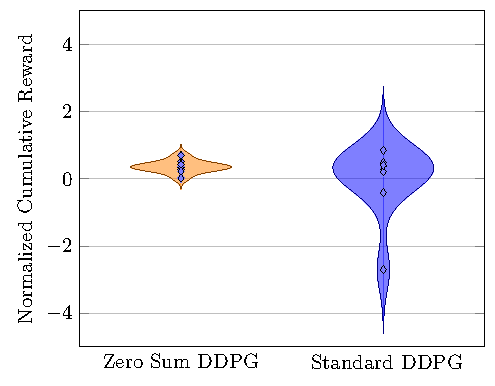
\includegraphics[width=0.6\textwidth]{plots/ddpg/violin_plot/initial_condition_shift}
%	\caption{مقایسه مجموع پاداش دو الگوریتم تک‌عاملی و چندعاملی \lr{DDPG} در شرایط اولیه تصادفی}
%\end{figure}
%
%\begin{figure}[H]
%	\centering
%	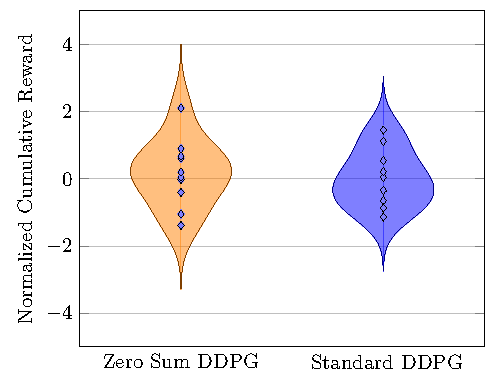
\includegraphics[width=0.6\textwidth]{plots/ddpg/violin_plot/actuator_disturbance}
%	\caption{مقایسه مجموع پاداش دو الگوریتم تک‌عاملی و چندعاملی \lr{DDPG} در حضور اغتشاش در عملگرها}
%\end{figure}
%
%\begin{figure}[H]
%	\centering
%	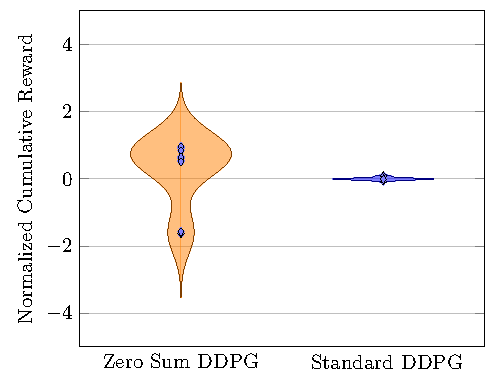
\includegraphics[width=0.6\textwidth]{plots/ddpg/violin_plot/model_mismatch}
%	\caption{مقایسه مجموع پاداش دو الگوریتم تک‌عاملی و چندعاملی \lr{DDPG} در مواجهه با عدم تطابق مدل}
%\end{figure}
%
%\begin{figure}[H]
%	\centering
%	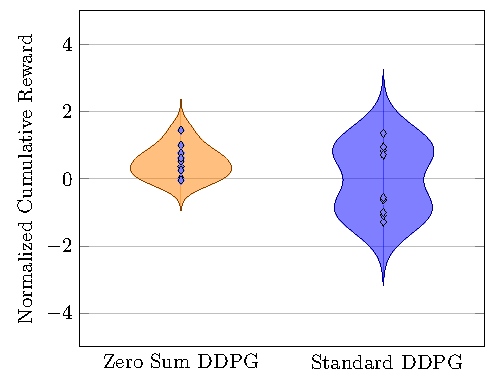
\includegraphics[width=0.6\textwidth]{plots/ddpg/violin_plot/partial_observation}
%	\caption{مقایسه مجموع پاداش دو الگوریتم تک‌عاملی و چندعاملی \lr{DDPG} در شرایط مشاهده ناقص}
%\end{figure}
%
%\begin{figure}[H]
%	\centering
%	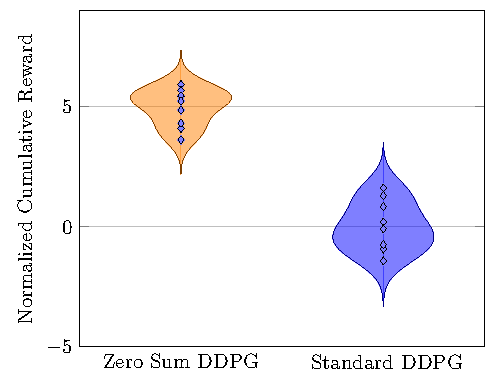
\includegraphics[width=0.6\textwidth]{plots/ddpg/violin_plot/sensor_noise}
%	\caption{مقایسه مجموع پاداش دو الگوریتم تک‌عاملی و چندعاملی \lr{DDPG} در حضور نویز حسگر}
%\end{figure}
%
%\begin{figure}[H]
%	\centering
%	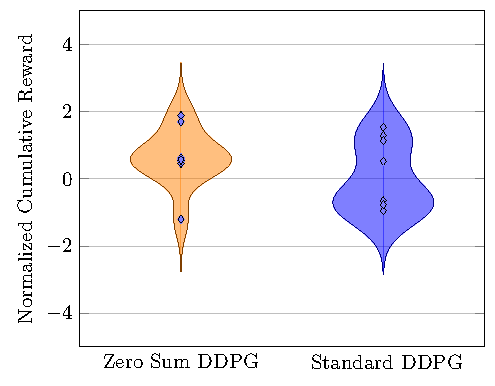
\includegraphics[width=0.6\textwidth]{plots/ddpg/violin_plot/time_delay}
%	\caption{مقایسه مجموع پاداش دو الگوریتم تک‌عاملی و چندعاملی \lr{DDPG} در شرایط تأخیر زمانی}
%\end{figure}



\begin{figure}[H]
	\centering
	
	% سطر اول
	\subfloat[شرایط اولیه تصادفی]{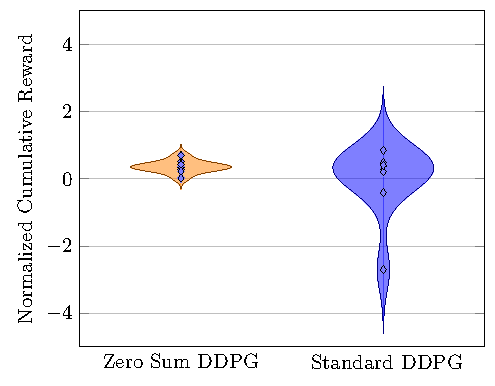
\includegraphics[width=.33\textwidth]{plots/ddpg/violin_plot/initial_condition_shift.pdf}}%
	\subfloat[اغتشاش در عملگرها]{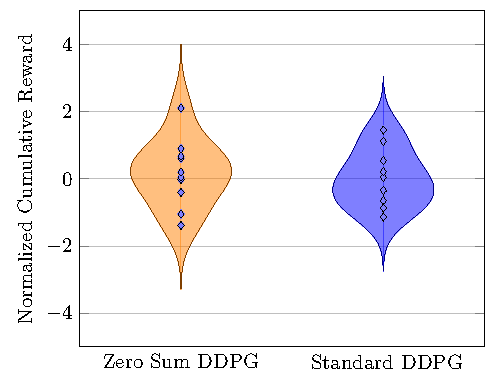
\includegraphics[width=.33\textwidth]{plots/ddpg/violin_plot/actuator_disturbance.pdf}}%
	\subfloat[عدم تطابق مدل]{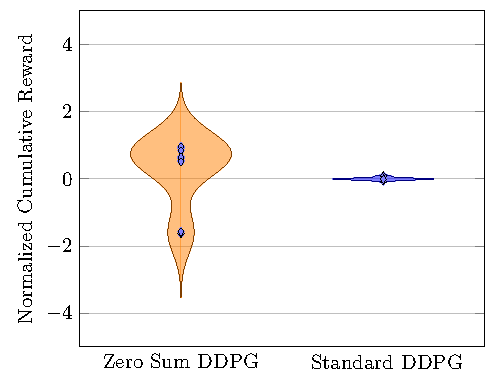
\includegraphics[width=.33\textwidth]{plots/ddpg/violin_plot/model_mismatch.pdf}}\\[1ex]
	
	% سطر دوم
	\subfloat[مشاهده ناقص]{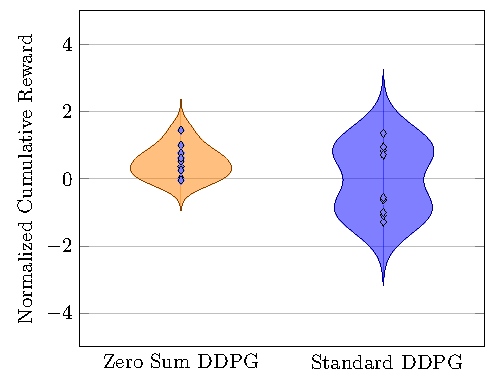
\includegraphics[width=.33\textwidth]{plots/ddpg/violin_plot/partial_observation.pdf}}%
	\subfloat[نویز حسگر]{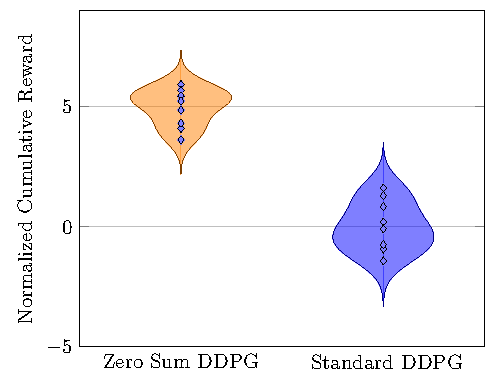
\includegraphics[width=.33\textwidth]{plots/ddpg/violin_plot/sensor_noise.pdf}}%
	\subfloat[تأخیر زمانی]{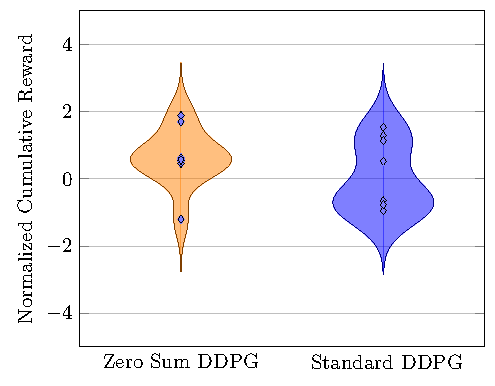
\includegraphics[width=.33\textwidth]{plots/ddpg/violin_plot/time_delay.pdf}}
	
	\caption{مقایسه مجموع پاداش دو الگوریتم تک‌عاملی و چندعاملی \lr{DDPG} در سناریوهای مختلف}
	\label{fig:ddpg_robustness_violin}
\end{figure}




\begin{figure}[H]
	\centering
	
	% سطر اول
	\subfloat[شرایط اولیه تصادفی]{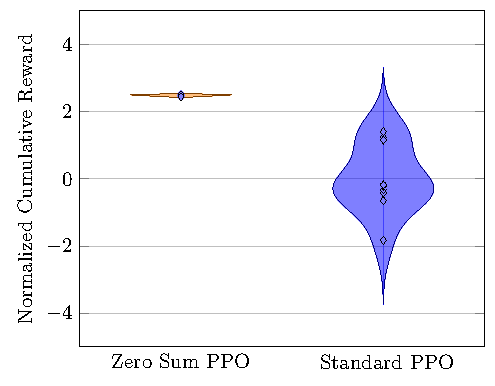
\includegraphics[width=.33\textwidth]{plots/ppo/violin_plot/initial_condition_shift.pdf}}%
	\subfloat[اغتشاش در عملگرها]{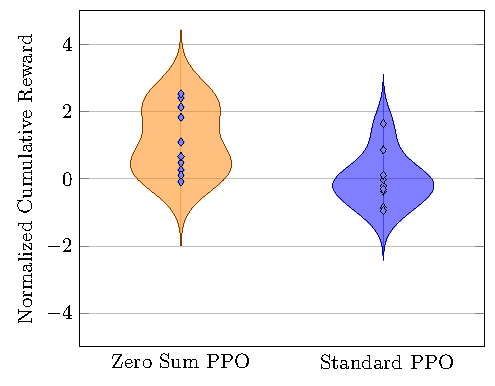
\includegraphics[width=.33\textwidth]{plots/ppo/violin_plot/actuator_disturbance.pdf}}%
	\subfloat[عدم تطابق مدل]{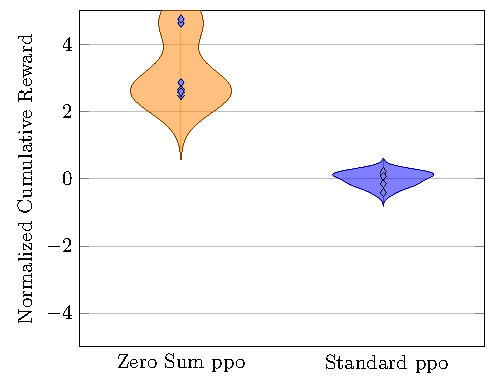
\includegraphics[width=.33\textwidth]{plots/ppo/violin_plot/model_mismatch.pdf}}\\[1ex]
	
	% سطر دوم
	\subfloat[مشاهده ناقص]{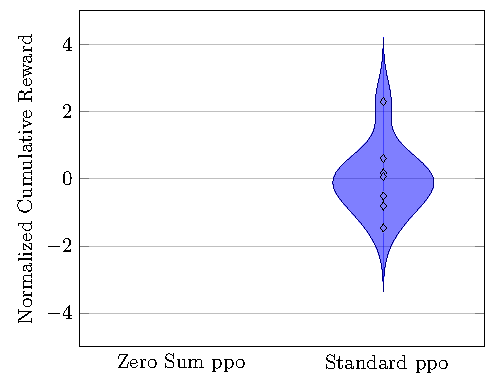
\includegraphics[width=.33\textwidth]{plots/ppo/violin_plot/partial_observation.pdf}}%
	\subfloat[نویز حسگر]{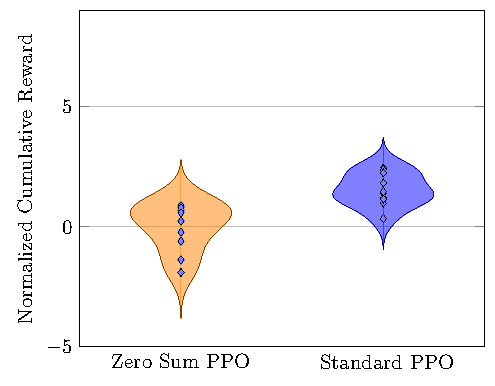
\includegraphics[width=.33\textwidth]{plots/ppo/violin_plot/sensor_noise.pdf}}%
	\subfloat[تأخیر زمانی]{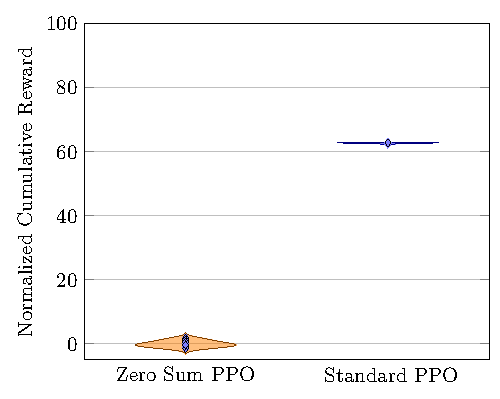
\includegraphics[width=.33\textwidth]{plots/ppo/violin_plot/time_delay.pdf}}
	
	\caption{مقایسه مجموع پاداش دو الگوریتم تک‌عاملی و چندعاملی \lr{PPO} در سناریوهای مختلف}
	\label{fig:ppo_robustness_violin}
\end{figure}





\begin{figure}[H]
	\centering
	
	% سطر اول
	\subfloat[شرایط اولیه تصادفی]{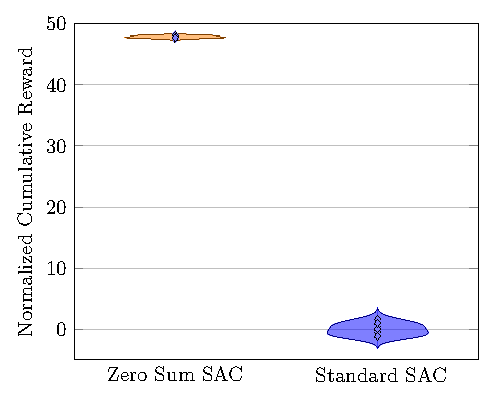
\includegraphics[width=.33\textwidth]{plots/sac/violin_plot/initial_condition_shift.pdf}}%
	\subfloat[اغتشاش در عملگرها]{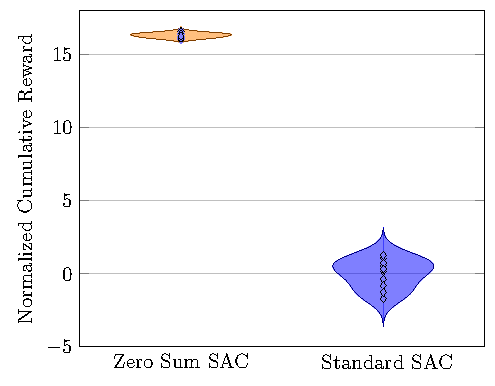
\includegraphics[width=.33\textwidth]{plots/sac/violin_plot/actuator_disturbance.pdf}}%
	\subfloat[عدم تطابق مدل]{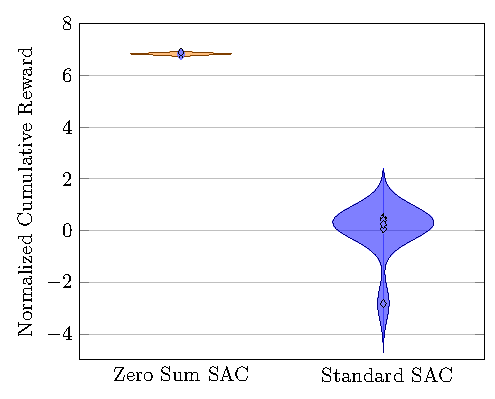
\includegraphics[width=.33\textwidth]{plots/sac/violin_plot/model_mismatch.pdf}}\\[1ex]
	
	% سطر دوم
	\subfloat[مشاهده ناقص]{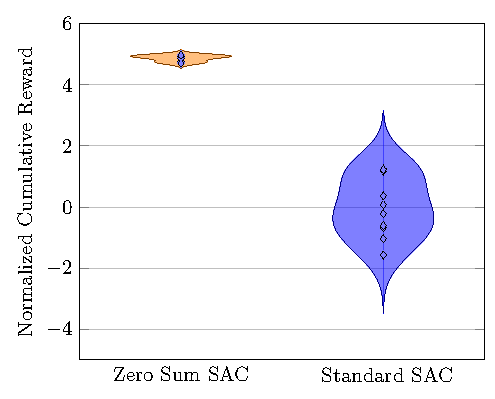
\includegraphics[width=.33\textwidth]{plots/sac/violin_plot/partial_observation.pdf}}%
	\subfloat[نویز حسگر]{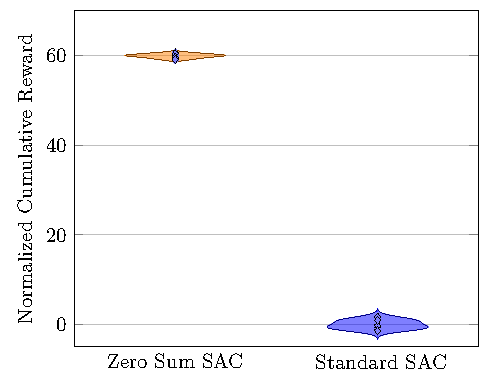
\includegraphics[width=.33\textwidth]{plots/sac/violin_plot/sensor_noise.pdf}}%
	\subfloat[تأخیر زمانی]{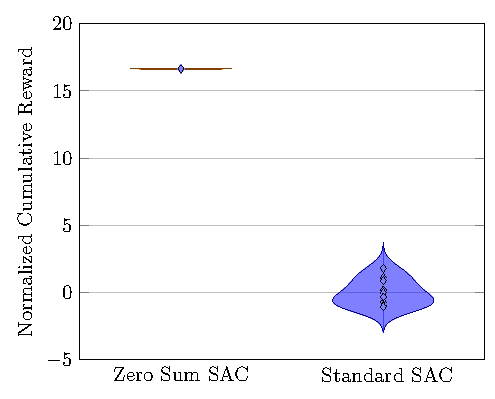
\includegraphics[width=.33\textwidth]{plots/sac/violin_plot/time_delay.pdf}}
	
	\caption{مقایسه مجموع پاداش دو الگوریتم تک‌عاملی و چندعاملی \lr{SAC} در سناریوهای مختلف}
	\label{fig:sac_robustness_violin}
\end{figure}
% Chapter 9: Conclusion
% -------------------------------------------------------
%  Conclusion
% -------------------------------------------------------

\chapter{نتیجه‌گیری و پیشنهادها}
\label{chap:conclusion}

\noindent
در این پایان‌نامه، مسأله‌ی هدایتِ مقاومِ فضاپیماهای کم‌پیشران در دینامیکِ چندجسمیِ مدلِ \lr{CRTBP} زمین–ماه به‌صورت یک {بازی دیفرانسیلی مجموع‌صفر} میان عامل هدایت و عامل مزاحم صورت‌بندی شد و با الگوی {آموزش متمرکز–اجرای توزیع‌شده} دنبال گردید. چهار الگوریتم پیوسته‌ی \lr{DDPG}، \lr{TD3}، \lr{SAC} و \lr{PPO} به نسخه‌های چندعاملیِ مجموع‌صفر تعمیم داده شدند، اجزای بازیگر–منتقد و سازوکارهای پایداری آموزش تشریح گردید. ارزیابی گسترده زیر عدم‌قطعیت‌های واقع‌گرایانه شرایط اولیه‌ی تصادفی، اغتشاش عملگر، نویز حسگر، تأخیر زمانی و عدم‌تطابق مدل نشان داد نسخه‌های مجموع‌صفر به‌صورت پایدار از همتایان تک‌عاملی پیشی می‌گیرند؛ به‌ویژه \lr{MA-TD3} بهترین سازش میان دقت مسیر، مصرف سوخت و پایداری را فراهم کرد.

\section*{جمع‌بندی دستاوردها}
\begin{itemize}
  \item ارائه‌ی صورت‌بندی بازی دیفرانسیلی مجموع‌صفر برای هدایت کم‌پیشران در \lr{CRTBP} با آموزش متمرکز و اجرای توزیع‌شده.
  \item تعمیم چهار الگوریتم پرکاربرد \lr{RL} به نسخه‌های چندعاملی مجموع‌صفر و تبیین دقیق معماری بازیگر–منتقد و پایدارسازی آموزش.
  \item طراحی حریفِ یادگیر برای تنوع‌بخشی نظام‌مند به عدم‌قطعیت‌ها و ارتقای تاب‌آوری سیاست در سناریوهای دشوار.
  \item پروتکل ارزیابی چندمعیاره با شاخص‌های دقت مسیر، پاداش 
  و پایداری، و نشان‌دادن برتری
   منسجم نسخه‌های مجموع‌صفر.
%  \item پیاده‌سازی سبک‌وزن و قابل‌اجرا به‌صورت بلادرنگ با کوانتیزاسیون \lr{INT8} با افت دقت ناچیز.
\end{itemize}

%\section*{محدودیت‌ها}
%\begin{itemize}
%  \item تحلیل در چارچوب \lr{CRTBP} انجام شد؛ تعمیم کامل به میدان‌های چندجسمیِ مبتنی بر اپمریس یا اثرات غیرمداری (تابش خورشیدی، سایه، محدودیت توان/حرارت) مستلزم توسعه‌ی مدل است.
%  \item سناریوهای عدم‌قطعیت عمدتاً به‌صورت مستقل آزموده شدند؛ ارزیابی هم‌زمانِ ترکیبات شدیدتر می‌تواند تصویر محافظه‌کارانه‌تری ارائه دهد.
%  \item حساسیت به طراحی و مقیاس‌بندی پاداش و تنظیمات \lr{RL}؛ نیاز به مطالعه‌ی نظام‌مند حساسیت و ابلیشن برای جداسازی عوامل اثرگذار.
%  \item هزینه‌ی آموزش و نمونه‌کارایی: بودجه‌ی محاسباتی بالا و نوسان عملکرد نسبت به بذرهای تصادفی می‌تواند بازتولید را دشوار کند.
%  \item تضمین‌های نظری محدود درباره‌ی ایمنی و بهینگی در حضور تأخیر و عدم‌تطابق مدل؛ نیاز به چارچوب‌های رسمی‌تر.
%\end{itemize}

\section*{پیشنهادهایی برای کارهای آینده}
\begin{itemize}
	\item تعمیم چارچوب به مسئله \lr{$N$-body} و درنظرگرفتن اغتشاشات غیرگرانشی؛ استفاده از یادگیری مرحله‌ای (\lr{curriculum}) متناسب با پیچیدگی دینامیکی.
	\item بررسی \lr{Risk-Sensitive RL}، اعمال قیود ایمنی به‌صورت \lr{chance constraints} و به‌کارگیری \lr{Control Barrier Functions}
	 برای فراهم‌کردن تضمین.
	\item توسعه راهبردهای ترکیبی یادگیری تقویتی و کنترل مبتنی بر مدل (مانند \lr{MPC}/\lr{iLQR}) برای بهبود ایمنی و تفسیرپذیری.
	\item آموزش خصمانه مبتنی بر توزیع (جمعیت مزاحم‌ها) و طراحی \lr{curriculum/adversary shaping} برای پوشش بهتر نواحی عدم‌قطعیت.
	\item استقرار روی سامانه‌های تعبیه‌شده‌ی کم‌مصرف و مقایسه‌ی \lr{ONNX Runtime}، \lr{TVM} و \lr{TensorRT} در معماری‌های گوناگون؛ بهینه‌سازی \lr{latency/throughput} و سنجه‌ی \lr{energy–delay}.
	\item انجام تحلیل حساسیت نسبت به تابع پاداش، معماری، نویز حسگر و تأخیر؛ مستندسازی دقیق برای ارتقای بازتولیدپذیری.
\end{itemize}
       

\vspace{0.5em}
در مجموع، نتایج این پژوهش نشان داد که رویکرد بازی‌محور چندعاملی در یادگیری تقویتی می‌تواند هدایت تطبیقی و مقاوم را بدون اتکای شدید به مدل‌های دقیق فراهم کند و مسیر روشنی برای گذار به کاربردهای عملی و سناریوهای پیچیده‌تر می‌گشاید.



%\section{سندباکس}


\begin{tikzpicture}
	\begin{axis}[
		% xmode=log,
		% ymode=log,
		legend style={at={(1,1)},anchor=north east
			,draw=none,fill=none,inner sep=2mm},
		xlabel=X, % \hertz requires SIunits
		ylabel=Y,
		title={Trajectory of the satellite},
		% grid=both,
		% minor grid style={gray!25},
		% major grid style={gray!25},
		width=0.75\linewidth,
		enlarge y limits=0.15,
		no marks]
		\addplot[line width=1pt,solid,color=blue] %
		table[x=x,y=y,col sep=comma]{../Code/Python/Environment/trajectory_latex.csv};
		\addlegendentry{Trajectory}
	\end{axis}
\end{tikzpicture}


% -------------------- Bibliography & Dictionary --------------------


% -------------------------------------------------------
%  Bibliography
% -------------------------------------------------------


\begin{latin}
%	\renewcommand{\bibname}{\rl{مراجع}}
\baselineskip=.8\baselineskip
\bibliographystyle{./styles/packages/unsrtabbrv}

% Uncomment next line to include uncited references
% \nocite{*}

\bibliography{bibs/full,bibs/refs}
 
\end{latin}
\newpage

\include{front/dictionary}


% -------------------- Appendices --------------------

\begin{appendix}
\include{chapters/appendix}
\end{appendix}


% -------------------- English Pages --------------------

%\newgeometry{left=3cm,right=2.5cm}


% -------------------------------------------------------
%  English Abstract
% -------------------------------------------------------


\pagestyle{empty}

\begin{latin}
	
	\begin{center}
		\textbf{Abstract}
	\end{center}
	\baselineskip=.8\baselineskip
	\noindent
	
%	In this study, a quadcopter stand with three degrees of freedom was controlled using game theory-based control. The first player tracks a desired input, and the second player creates a disturbance in the tracking of the first player to cause an error in the tracking. The move is chosen using the Nash equilibrium, which presupposes that the other player made the worst move.. In addition to being resistant to input interruptions, this method may also be resilient to modeling system uncertainty. This method evaluated the performance through simulation in the Simulink environment and implementation on a three-degree-of-freedom stand.
This thesis proposes a robust guidance framework for low‑thrust spacecraft operating in multi‑body dynamical environments modeled by the Earth–Moon circular restricted three‑body problem (CRTBP). The guidance task is cast as a zero‑sum differential game between a controller agent (spacecraft) and an adversary agent (environmental disturbances), implemented under a centralized‑training/ decentralized‑execution paradigm. Four continuous‑control reinforcement‑learning algorithms—DDPG, TD3, SAC, and PPO—are extended to their multi‑agent zero‑sum counterparts (MA‑DDPG, MATD3, MASAC, MAPPO); their actor–critic network structures and training pipelines are detailed.

The policies are trained and evaluated on transfers to the Earth–Moon  lyapunov orbit under five uncertainty scenarios: random initial states, actuator perturbations, sensor noise, communication delays, and model mismatch. Zero‑sum variants consistently outperform their single‑agent baselines, with MATD3 delivering the best trade‑off between trajectory accuracy and propellant consumption while maintaining stability in the harshest conditions.

For real‑time deployment, the learned networks are quantized to INT8 and exported to ONNX for execution on a ROS 2 hardware‑in‑the‑loop platform. Inference latency is reduced to 5.8 ms and memory footprint to 9.2 MB—improvements of 47 \% and 53 \% over the FP32 models—while sustaining a 100 Hz control loop with no deadline misses.

The results demonstrate that the proposed multi‑agent, game‑theoretic reinforcement‑learning framework enables adaptive and robust low‑thrust guidance in unstable three‑body regions without reliance on precise dynamics models, and is ready for hardware‑in‑the‑loop implementation.

	
	\bigskip\noindent\textbf{Keywords}:
%	Quadcopter, Differential Game, Game Theory, Nash Equilibrium, Three Degree of Freedom Stand, Model Base Design, Linear Quadratic Regulator
	Deep Reinforcement Learning; Differential Game; Multi‑Agent; Low‑Thrust Guidance; Three‑Body Problem; Robustness.
\end{latin}

\newpage
\pagestyle{empty}

\begin{center}

\begin{latin}


\includegraphics[scale=0.25]{front/template/images/logo}

\EnglishThesisUniversity \\
\EnglishThesisDepartment

\begin{large}
\vspace{0.2cm}
\EnglishThesisType


\vspace{1cm}

{\Large\textbf{\EnglishThesisTitle}}

\vspace{1cm}

{\normalsize By:}\\
\textbf{\EnglishThesisAuthor}

\vspace{0.8cm}

{\normalsize Supervisor:}\\ 
\textbf{\EnglishThesisSupervisor}

\end{large}

\vspace{1.5cm}
\EnglishThesisDate

\end{latin}

\end{center}



% -------------------- The End! --------------------

\end{document}
